\documentclass[12pt,a4paper]{report}


% --- Langue / encodage ---
\usepackage[T1]{fontenc}
\usepackage[utf8]{inputenc} % OK avec pdflatex
\usepackage[french]{babel}

\addto\captionsfrench{%
	\renewcommand{\figurename}{Carte}%
	\renewcommand{\listfigurename}{Liste des cartes}%
}

% --- Mise en page minimale ---
\usepackage[a4paper,margin=2.5cm]{geometry}
\usepackage{microtype}
\usepackage{lmodern}
\sloppy

% --- Autorise les underscores dans le texte ---
\usepackage[strings]{underscore}

% --- Figures / tableaux ---
\usepackage{graphicx}
\usepackage{booktabs}
\usepackage{longtable}
\usepackage{float}


% --- Hyperliens (ne charger QU'UNE fois) ---
\usepackage[hypertexnames=false]{hyperref}
\hypersetup{
	colorlinks=true,
	linkcolor=blue,
	urlcolor=blue,
	citecolor=blue
}

% --- Bibliographie en notes complètes ---
\usepackage{csquotes}
\usepackage{xurl} % coupe mieux les URL
\usepackage[
backend=biber,
style=verbose-trad2,
citetracker=true
]{biblatex}
\addbibresource{bibliographie.bib}

%Pour annexe Affranchissement

\usepackage{marginnote}
%\usepackage{ulem} %pour les caractères barrés

\usepackage{glossaries}
\makeglossaries

\newglossaryentry{rière}
{
	name=rière,
	description={"dans le territoire de"}
}
\newglossaryentry{cens}
{
	name=cens,
	description={Le cens est dû par celui qui a la propriété utile d'un bien foncier (généralement un paysan) à celui qui en a la propriété éminente (le seigneur, qui à l'Époque moderne n'est pas nécessairement un noble)}
}
\newglossaryentry{servis}
{
	name=servis,
	description={"Les servis, appelés aussi censes, correspondent à des redevances annuelles et doivent être
		payés perpétuellement au seigneur, en sus des frais d’acquisition (introge) d’une terre
		dépendante de la seigneurie. Ils peuvent être dûs en argent, mais souvent en nature, redevances
		en blé par exemple, ou autres denrées. Les servis pèsent parfois très lourds eu égard à la
		rentabilité de la terre. Ces redevances seigneuriales, s’apparentant à une sorte de bail
		emphytéotique, s’ajoutent aux tailles, gabelles, dîmes et autres impôts"\footnote{\cite{Gachet2022}}}
}
\newglossaryentry{laodsindemnité}
{
	name=laods d'indemnité,
	description={Somme versée en compensation des droits de lods lorsque ceux-ci sont rachetés, supprimés ou convertis en indemnité forfaitaire.}
}
\newglossaryentry{laods}
{
	name=laods,
	description={"Les loads sont des droits de mutations perçus par un seigneur lors de la vente d’une terre par
		un de ses sujets. Ils sont payés par l’acheteur. S’ils constituent une protection contre la
		spéculation foncière des plus riches, ils sont aussi un frein aux acquisitions par les plus pauvres,
		aux remembrements et à l’optimisation du travail des terres. Ils peuvent se monter jusqu’à un
		sixième de la valeur des transactions.
		Les loads et les servis concernent toutes les personnes qui ont acquis des biens fonciers
		dépendant du fief d’un seigneur. A noter que le seigneur peut être une personne physique mais
		également une abbaye, un évêché etc. Etre dépendant d’un fief ne signifie pas dans tous les cas
		une dépendance personnelle envers le seigneur, ni forcément l’appartenance à une classe sociale
		inférieure. Ceux qui dépendent personnellement d’un seigneur et qui sont de catégorie sociale
		inférieure sont les personnes dites taillables, mainmortables ou corvéables à merci. On utilise
		peu le terme de serf à l’époque moderne en Savoie. Sur ces personnes pèsent des charges
		seigneuriales supplémentaires, notamment des corvées, et surtout le droit d’échute." \footnote{\cite{Gachet2022}} }
}

\newglossaryentry{suffertes}
{
	name=suffertes,
	description={droit de mutation que l'on percevait en sus du laod quand un fonds taillable était vendu à un homme de condition non taillable ou quand un fonds franc était acheté par un homme taillable}
}
\newglossaryentry{dîmes}
{
	name=dîmes,
	description={redevance en nature ou en argent, portant principalement sur les revenus agricoles collectés en faveur de l’Église}
}
\newglossaryentry{décimes}
{
	name=décimes,
	description={voir dîme}
}
\newglossaryentry{corvées}
{
	name=corvées,
	description={"Les corvées sont des prestations périodiques dues aux seigneurs par leurs sujets. Il peut s’agir
		de labours de terres, de coupes de bois, de transports de matériaux etc. Selon leur nature elles
		peuvent être intégrées aux servis sans faire l’objet d’une terminologie à part" \footnote{\cite{Gachet2022}}}
}

\newglossaryentry{droits de haut siège}
{
	name=droits de haut siège,
	description={Droits attachés à la haute justice seigneuriale, comprenant notamment le pouvoir de juger les crimes les plus graves et d'exercer les peines capitales.}
}
\newglossaryentry{favettiers}
{
	name=favettiers,
	description={(Savoie) (Droit) Paysans, bourgeois, gentilhommes assujettis aux redevances seigneuriales (load, sufferte, plaid, corvée, cens). }
}
\newglossaryentry{égances}
{
	name=égances,
	description={fractionnement des charges foncières lors du partage d’une censive}
}
\newglossaryentry{péages}
{
	name=péages,
	description={Droits perçus sur les personnes, les animaux ou les marchandises empruntant une route, un pont ou un passage relevant d'un seigneur ou d'une autorité publique.}
}


\newglossaryentry{bans champêtres}
{
	name=bans champêtres,
	description={bans de justice, voir aussi \cite{Berthier}}
}

\newglossaryentry{remèdes possessoriaux}
{
	name=remèdes possessoriaux,
	description={Procédures judiciaires destinées à protéger la possession d'un bien indépendamment de la question de la propriété.}
}

\newglossaryentry{bénéfices d'instances}
{
	name=bénéfices d'instances,
	description={Privilèges procéduraux permettant à une partie d'obtenir certains avantages dans le déroulement d'une instance judiciaire.}
}

\newglossaryentry{rescindants}
{
	name=rescindants,
	description={Demande tendante à faire annuler un acte, un jugement. On a jugé le rescindant. Par cet arrêt, on n’a jugé que le rescindant. Nous avons gagné le rescindant, c’est une présomption en notre faveur pour le rescisoire}
}

\newglossaryentry{rescisoire}
{
	name=rescisoire,
	description={L’objet principal pour lequel on s’est pourvu, soit contre un acte, soit contre un jugement, et qui reste à juger, quand l’acte ou le jugement a été annulé. Le rescindant et le rescisoire ne sont pas jugés par le même arrêt}
}
\newglossaryentry{droit de pignoratitie}
{
	name=droit de pignoratitie,
	description={Pignoratif ? Qui est relatif à un gage. Endossement pignoratif, qui transfère à l’endossataire les droits d’un créancier gagiste. Vieilli. Contrat pignoratif, forme de contrat de vente à réméré qui, dissimulant un prêt sur gage et s’apparentant à un pacte commissoire, est prohibée par la loi.}
}
\newglossaryentry{nomination des officiers de justice}
{
	name=nomination des officiers de justice,
	description={le chatelain (souvent un notaire) est choisi par le seigneur pour le représenter sur son fief qui lui délègue notamment le rôle d'officier de basse justice}
}

\newglossaryentry{greffe}
{
	name=greffe,
	description={Bureau où sont conservés les actes, registres et décisions d'une juridiction ; par extension, ensemble des archives judiciaires.}
}
\newglossaryentry{leyde sur le bétail}
{
	name=leyde sur le bétail,
	description={La leyde était sous l'Ancien Régime en France (surtout au Moyen Âge) un droit féodal, sous la forme d'impôt, levé sur les marchandises, denrées et bestiaux vendus en foire et marché}
}


\newglossaryentry{hale}
{
	name=hale,
	description={Probablement une halle : bâtiment public destiné à la tenue des marchés et des foires.}
}


\newglossaryentry{mense archiépiscopale}
{
	name=mense archiépiscopale,
	description={ revenus liés aux possessions du clergé. On parle de Mense curiale, monacale, abbatiale, épiscopale. C’est un revenu destiné à la subsistance des ecclésiastiques, aux besoins du culte, à l’entretien des biens et de l’assistance aux pauvres.}
}
\newglossaryentry{droit des langues dû par les bouchers}
{
	name=droit des langues dû par les bouchers,
	description={est un "prélèvement en nature des langues de boeufs et de vaches, et même parfois de tous les autres animaux abattus par les bouchers, ce droit est le plus souvent remplacé par une indemnité annuelle compensatrice" cf G Sangnier}
}
\newglossaryentry{recherche des cristaux}
{
	name=recherche des cristaux,
	description={droit coutumier local, le seigneur se réservant les cristaux trouvés sur son territoire}
}
\newglossaryentry{droit d’avoir un banc placé}
{
	name=droit d’avoir un banc placé,
	description={Privilège honorifique permettant au seigneur ou à une famille de disposer d'un banc réservé dans l'église paroissiale.}
}
\newglossaryentry{placer des patibulaires avec ses armoiries}
{
	name=placer des patibulaires avec ses armoiries,
	description={est un moyen pour le seigneur d'un lieu de marquer son pouvoir de justice (haute, moyenne ou basse}
}
\newglossaryentry{échute}
{
	name=placer des patibulaires avec ses armoiries,
	description={"Dans les procès et les débats qui ont régulièrement eu lieu entre les promoteurs
		d’affranchissements des « mainmortables » et leurs détracteurs, c’est sur le droit d’échute
		semble-t-il qu’on s’oppose le plus radicalement. En quoi consiste-t-il ? C’est le droit de
		propriété qu’un seigneur peut avoir sur les biens de ses sujets « taillables », lorsque ceux-ci
		décèdent sans héritiers « directs » (enfants mâles en général). Des coutumes régionales peuvent
		différer : en certains lieux ce ne sera pas la totalité des biens mais une partie seulement, en
		d’autres endroits l’existence de filles au décès pourra aussi moduler le droit d’échute, etc.
		Comme souvent sous l’ancien régime, pas de règle universelle sans particularités locales. Mais
		l’esprit est là : impossible à un serf de disposer et de tester librement de ses biens. D’où l’origine
		possible du mot « mainmortable », qui aurait la main morte, incapable de coucher par écrit un
		testament.
		Ce droit d’échute est d’autant plus mal vécu qu’il s’applique même sur des biens acquis à
		l’extérieur de la seigneurie. Ces mainmortables – taillables ou serfs – font également l’objet de
		mesures vexatoires : certaines fonctions ou certaines tenues vestimentaires leurs sont interdites." \footnote{\cite{Gachet2022}} }
}

\newglossaryentry{échuttes}
{
	name=échuttes,
	description={voir échute }
}

\newglossaryentry{terriers}
{
	name=terriers,
	description={registre contenant les lois et usages d'une seigneurie, la description des bien-fonds, les droits et conditions des personnes, ainsi que les redevances et obligations auxquelles elles sont soumises}
}
\newglossaryentry{litterés}
{
	name=litterés,
	description={autres écrits}
}
\newglossaryentry{doages}
{
	name=doages,
	description={Biens ou revenus constituant le douaire, c'est-à-dire les droits assurant la subsistance d'une veuve.}
}
\newglossaryentry{banc du droit}
{
	name=banc du droit,
	description={Lieu où se tenaient les audiences de la justice seigneuriale et, par extension, les assemblées publiques de la communauté.}
}
\newglossaryentry{prône}
{
	name=prône,
	description={Instruction, accompagnée d'avis, qu'un prêtre fait aux fidèles à la messe paroissiale du dimanche}
}
\newglossaryentry{droit de reachapt}
{
	name=droit de reachapt,
	description={droit de réachat}
}
\newglossaryentry{Laide}
{
	name=Laide,
	description={ pour Leyde ? La leyde était sous l'Ancien Régime en France (surtout au Moyen Âge) un droit féodal, sous la forme d'impôt, levé sur les marchandises, denrées et bestiaux vendus en foire et marché}
}
\newglossaryentry{droit de pêche de chasse}
{
	name=droit de pêche de chasse,
	description={Droit exclusif accordé au seigneur d'exercer ou d'autoriser la chasse et la pêche sur les terres et les eaux de sa juridiction.}
}

% Glossaire pour Litige Traicol
\newglossaryentry{communaux}{name=communaux,description={Biens collectifs dont l'usage appartient à une communauté d'habitants, notamment pour le pâturage, le bois ou d'autres usages ruraux.}}
\newglossaryentry{fondspropres}{name=fonds propres,description={Biens possédés à titre particulier, par opposition aux communaux.}}
\newglossaryentry{albergement}{name=albergement,description={Contrat de concession, fréquent dans les pays savoyards, par lequel un seigneur concède un bien ou un droit moyennant redevance et reconnaissance.}}
\newglossaryentry{domaineDirect}{name=domaine direct,description={Droit éminent conservé par le seigneur sur un bien concédé à un tenancier ou à une communauté.}}
\newglossaryentry{reconnaissance}{name=reconnaissance,description={Acte par lequel un tenancier reconnaît tenir un bien ou un droit d'un seigneur, avec indication des charges dues.}}
\newglossaryentry{prescription}{name=prescription,description={Mode d'acquisition ou de consolidation d'un droit par l'effet d'une possession prolongée et non interrompue.}}
\newglossaryentry{possessionImmemoriale}{name=possession immémoriale,description={Possession si ancienne qu'elle est réputée excéder la mémoire des hommes et peut, dans l'argumentation judiciaire, tenir lieu de preuve.}}
\newglossaryentry{mappe}{name=mappe,description={Plan cadastral dressé lors de la mensuration générale des États de Savoie au XVIIIe siècle.}}
\newglossaryentry{mensurationGenerale}{name=mensuration générale,description={Opération cadastrale menée dans les États de Savoie afin de mesurer les biens et d'établir la mappe et les registres cadastraux.}}
\newglossaryentry{lettresPatentes}{name=lettres patentes,description={Acte souverain ouvrant ou autorisant une procédure, une concession ou une décision administrative.}}
\newglossaryentry{confrerieSaintEsprit}{name=confrérie du Saint-Esprit,description={Institution confraternelle détenant ici des biens dans la vallée de Treicol, administrés par les syndics et conseil des Chapelles.}}
\newglossaryentry{leyde}{name=leyde,description={Droit perçu sur certaines marchandises, denrées ou bestiaux, notamment dans le cadre de foires, marchés ou usages seigneuriaux.}}
\newglossaryentry{alpeage}{name=alpéage,description={Redevance liée à l'usage des alpages ou montagnes pastorales.}}
\newglossaryentry{eauxPendantes}{name=eaux pendantes,description={Ligne de partage des eaux utilisée comme critère de délimitation territoriale en zone de montagne.}}


\newglossaryentry{introge}
{
	name=introge,
	description={Droit d'entrée payé au seigneur lors de l'acquisition d'une censive ou d'un bien relevant de sa seigneurie. Il est acquitté une seule fois, contrairement aux servis qui sont des redevances annuelles.}
}
\newglossaryentry{alpéages}
{
	name=alpéages,
	description={voir auciège}
}

\newglossaryentry{auciège}
{
	name=auciège,
	description={Redevance seigneuriale due pour l'usage d'un alpage, généralement acquittée en produits laitiers correspondant au lait d'un ou plusieurs jours. Également appelé alpéage. Pour une étude sur l'auciège voir \cite{Duparc}}
}

\newglossaryentry{mainmorte}
{
	name=mainmorte,
	description={Condition juridique limitant les droits successoraux des sujets mainmortables et permettant notamment au seigneur d'exercer le droit d'échute dans certains cas.}
}

% --- Index multiples ---
\usepackage{imakeidx}

\makeindex[name=nom,     title={Index des noms}]
\makeindex[name=tab,     title={Index des tableaux}, columns=1]
\makeindex[name=carte,   title={Index des cartes et illustrations}, columns=1]


% --- Commandes d’indexation ---
\newcommand{\idxnom}[1]{\index[nom]{#1}}


%\newcommand{\idxtab}[1]{\index[tab]{#1}}
\newcommand{\idxcarte}[1]{\index[carte]{#1}}


\renewcommand{\figurename}{Fig.}

% --- Helpers pour légendes + index ---

% Table : caption + label + index "tab"
%\newcommand{\tabcaptionindex}[2]{%
%	\caption{#2}\label{#1}\idxtab{#2|hyperpage}%
%	\idxtab{Tableau \thetable\space -- #2|hyperpage}%
%}
\newcommand{\tabcaptionindex}[2]{%
	\caption{#2}%
	\label{#1}%
	\index[tab]{%
		\thechapter.\ifnum\value{table}<10 0\fi\arabic{table}%
		@Tableau~\thetable\space--\space #2|hyperpage%
	}%
}

%old Figure : caption + label + index selon type ("carte" ou "image")
% Usage : \figcaptionindex{carte}{fig:...}{Texte}
\newcommand{\figcaptionindex}[3]{%
	\caption{#3}\label{#2}%
	\def\tempa{#1}\def\tempb{Carte}%
	\ifx\tempa\tempb
	\idxcarte{#3|hyperpage}%
	\else
	\def\tempb{image}%
	\ifx\tempa\tempb
	\idximage{#3|hyperpage}%
	\fi
	\fi
}

\usepackage{pdflscape}

% --- Macro figure simple (ta macro) ---
% IMPORTANT : l'argument optionnel doit être collé : \cartefigure[0.5\textwidth]{...}{...}{...}
\newcommand{\cartefigure}[4][0.7\textwidth]{%
	\begin{figure}[H]
		\centering
		\includegraphics[width=\textwidth]{#2}
		\caption{#4}
		\label{#3}
		% Index : "Carte 3.1 — Titre"
		\idxcarte{Fig.~\thefigure\space--\space #4|hyperpage}%
	\end{figure}%
}



%%%%%%%%%%%%%%%%%%%%%%%%%%%%%%%%%%%%%%%%%%%%%%%%%%%%%%%%%%%%%%%
\begin{document}
	
	\title{Propriété des alpages à Saint-Maxime de Beaufort au XVIIIe siècle}
	\author{Nicolas MORANE - étudiant M1 SDH Panthéon-Sorbonne}
	\date{4 Juillet 2026}
	\maketitle
	
	\tableofcontents
	
	
	
\chapter*{Remerciements}
\addcontentsline{toc}{chapter}{Remerciements}
	
	
	C'est vers le Beaufortain et vers ses habitants que je voudrais adresser en premier lieu mes remerciements. 
	Je remercie, aussi, mon épouse, étrangère à la montagne, d'avoir accepté et aimé à son tour cette vallée unique.
	Évidemment je remercie les conseils et enseignements de mes professeurs de la Sorbonne qui ont accepté dans ce cursus de Master, un étudiant plus tout jeune.
	Je remercie enfin, Philippe Matignon, descendant du "vieil allobroge", le sénateur Pierre Blanc, pour m'avoir dévoilé et permis d'utiliser ici, cette très grande carte, peinte sur toile qu'il a sortie d'une armoire de sa maison de Beaufort. 
	
	
\chapter*{Introduction}
\addcontentsline{toc}{chapter}{Introduction}


Dans la plus grande maison de Beaufort (autrefois Saint-Maxime de Beaufort) se trouve une grande toile enroulée sur elle-même. Lorsqu'on la déroule (1,40m sur 2m), on aperçoit des motifs peints à la main en couleur, représentant des parcelles et tout autour des listes de numéros associé à des personnes et de lieux. au sommet, un blason :

\cartefigure[0.8\textwidth]
{figures/4 Cartouche Entête.jpg}
{fig:CartoucheCarteBlanc}
{St Maxime de Beaufort
	Le Plan Géographique
	des biens fond que possède le Rd Jean Antoine Blanc tant
	en son chef que par indivis avec Dame Charlotte et Demoiselle
	Jacqueline Blanc ses nièces de même que ceux que
	possède Dame Françoise veuve de Me Michel Blanc
	Notaire en la paroisse de St Maxime
	de Beaufort avec les confins des dits biens
	le tout levé par le géomètre Estienne
	Jaquet sur la mappe originale dressé
	à l'occasion de la mesure générale de Savoye
	[illisible] 1729 et
	1730}

Nous avons donc : un plan dressé par un géomètre, une mention de la Mappe Sarde et plusieurs propriétaires d'une même famille : un prêtre, la veuve d'un notaire et ses deux filles.

Il s'agit clairement d'un objet destiné à être montré et à afficher la richesse et la notabilité de la famille (peut-être en raison de deux jeunes femmes à marier ?).

Le bourg de Saint-Maxime se situe au centre de la petite vallée du Beaufortain qui était exclusivement rural jusqu'à l'arrivée des sports d'hiver et des barrages hydrauliques. Adossée au massif du Mont-Blanc et entourée des vallées plus larges et plus fréquentées de la Tarentaise, de l'Arly. Les sommets qui l'entourent culminent à moins de 3,000m, le Doron, gros torrent, s'en échappe vers 800m d'altitude, en laissant les pentes douces avec d'immenses étendues de prairies et de forêts. 

Entre l'isolement et les hivers rigoureux et enneigés, il n'est pas facile d'imaginer la vie dans cette vallée autrement que difficile et pauvre. 
Et pourtant, nous avons cette carte ostentatoire.

\vspace{1em}

Pour asseoir son emprise directe sur ses sujets et pour mieux contrôler la levée de la taille,  Victor-Amédée II, duc de Savoie (et tout juste roi de Sardaigne) met en œuvre entre 1720 et 1730, une "mensuration générale" pour établir un cadastre couvrant toutes les paroisses du duché: c'est la Mappe Sarde à laquelle faisait référence la carte de la famille Blanc.   

Hélène VIALLET a écrit en 1993 un livre passionnant sur l'histoire du Beaufortain, où l'on peut apprendre que la paroisse de Saint-Maxime était une des plus peuplées et une des plus riches du duché de Savoie jusqu'au XVIIIe siècle et cela dès avant l'introduction dans la vallée du gruyère suisse (le fameux Beaufort, prince des gruyères selon Brillat-Savarin) .

Mais ce n'est qu'au cours des années 2000 que le travail de numérisation de la Mappe Sarde par Dominique BARBERO est devenu accessible pour l'historien et  plus de 400 communes de Savoie et de Haute-Savoie ont été ainsi traitées. La commune de Beaufort en fait partie. En exploitant ces données avec les outils dont nous disposons aujourd'hui, nous sommes en mesure d'apporter des éclairages approfondis aux travaux d'Hélène VIALLET sur la paroisse de Saint-Maxime du XVIIIe siècle. En passant, nous essayerons de replacer la carte privée de la famille Blanc dans son contexte.


Nous avons  pu obtenir de Dominique BARBERO, une copie de son travail sous la forme de 53 documents pdf contenant le tracé des parcelles tiré de la Mappe originale conservée aux Archives Départementales de Chambéry ainsi qu'un fichier Excel avec les informations des 19.791 parcelles relevées par les arpenteurs.

\vspace{1em}
La stratégie capitaliste de notables investissant dans la propriété des alpages d'altitude a commencé  en Gruyère avec l'apparition du fromage du même nom, par les bourgeois de Fribourg.

L'introduction du Gruyère dans le Beaufortain a suivi une logique semblable et si cette évolution est bien documentée pour la famille Blanc dans les travaux d'Hélène Viallet, il nous a paru intéressant d'avoir une vision plus précise des propriétaires des alpages : les registres de la Mappe Sarde ne donnent pas l'information sur l'altitude des parcelles. Un travail de géoréférencement a été mené par Dominique Barbéro mais le Cd qu'il a produit ne donne que des impressions pdf des cartes numérisées. 

Il m'est donc apparu intéressant de pouvoir calquer la Mappe Sarde sur les cartes IGN et de (re)géoréférencer les parcelles, afin d'identifier d'une manière ou d'une autre les parcelles situées en altitude. Une fois les parcelles localisées, en extraire celles qui sont en pré ou en pâturage avec le nom des propriétaires apporte une vraie valeur ajoutée à la lecture des données initiales.

Le roi de Piemont-Sardaigne et duc de Savoie, Charles-Emmanuel III de Savoie décide de permettre le rachat des droits féodaux par les communautés d’habitants par deux édits : l’édit du 20 janvier 1762, puis celui du 19 décembre 1771. Les communautés du Mandement de Beaufort comportant les quatre paroisses : Saint-Maxime de Beaufort, Hauteluce, Villard sur Doron et Queige (pour une partie seulement) ont devancé la promulgation de l'édit de 1771 puisqu'elles ont ensemble racheté dès 1770 les droits féodaux les concernant. Le financement de ce rachat a été possible par la vente aux enchères d'une partie des communaux. Dans les documents entourant la procédure des enchères, les parcelles mises en vente sont décrites avec leur numéro du cadastre sarde de 1730. Il a donc été possible, là aussi, de connaître quelles étaient celles concernant des alpages d'altitude.  


	
\chapter{Contexte}

Avant d'analyser la photographie de la propriété foncière que constitue la Mappe Sarde au début du XVIIIe siècle, il convient de replacer le Beaufortain dans son contexte géographique, politique et économique. La répartition des alpages, des communaux et des propriétés observée vers 1730 est en effet l'aboutissement d'évolutions parfois très anciennes touchant à la fois l'organisation de l'espace alpin, la construction de l'État savoyard et les transformations du pastoralisme de montagne.

\section{Le Beaufortain dans l'espace alpin}

\subsection{Une vallée de montagne à l'écart des grands axes}

Situé au cœur des Alpes du Nord, le Beaufortain apparaît aujourd'hui comme une vallée relativement enclavée. Son accès principal s'effectue par les gorges du Doron depuis Conflans, ancienne ville située au confluent de l'Arly et de l'Isère. Contrairement à la Maurienne ou à la Tarentaise, il ne commande aucun des grands passages reliant la France à l'Italie.

Cette situation ne doit cependant pas conduire à exagérer son isolement. Jusqu'au XIXe siècle, les déplacements s'effectuent essentiellement à pied ou à dos de mulet. Dans ces conditions, le franchissement des cols constitue une pratique ordinaire des populations montagnardes. Le col des Saisies, le col du Joly, le Cormet de Roselend ou encore le Cormet d'Arêches assurent les liaisons régulières du Beaufortain avec les vallées voisines.



Le Beaufortain ne se situe donc pas en dehors de l'espace alpin. Il participe pleinement aux échanges humains et économiques qui animent les montagnes savoyardes, même si ces circulations demeurent essentiellement régionales. Seules les conditions hivernales peuvent entraîner un isolement sévère des communautés.

À une échelle plus large, le Beaufortain appartient à un ensemble géographique dont la cohérence repose sur le contrôle des grands passages alpins. Depuis l'Antiquité, plusieurs itinéraires majeurs relient les plaines françaises à l'Italie du Nord. Le Grand-Saint-Bernard permet la liaison entre Genève et la Vallée d'Aoste, tandis que le Montgenèvre ouvre la route de Turin et du Piémont.

Le col du Mont-Cenis occupe longtemps une place particulière. Durant une grande partie du Moyen Âge, il constitue la principale voie de communication entre la France et l'Italie. Son importance contribue largement à l'essor de la maison de Savoie, qui bâtit progressivement sa puissance en contrôlant les vallées donnant accès à ces passages stratégiques.

Toutefois, à partir du XIIIe siècle, le développement des routes du Simplon puis du Saint-Gothard modifie les grands courants commerciaux européens. Une partie croissante des échanges entre l'Italie et l'Europe du Nord emprunte alors des itinéraires plus orientaux.\footcite[63--82]{PRacine2003}

\cartefigure
{figures/0_Vue Aérienne Alpes.jpg}
{fig:VueAerienne}
{Vue aérienne des Alpes occidentales (Geoportail)}

Cette évolution contribue à marginaliser certains espaces alpins occidentaux. Le Beaufortain demeure cependant intégré aux réseaux régionaux d'échanges qui structurent les Alpes du Nord.

\section{L'intégration du Beaufortain aux États de Savoie}

À partir du XIIIe siècle, les comtes de Savoie construisent progressivement un État territorial cohérent à partir d'un ensemble de seigneuries jusque-là dispersées. Cette construction repose sur l'acquisition, l'échange ou la vassalisation de nombreux territoires alpins ainsi que sur la création d'une administration de plus en plus structurée.\footcite[59]{Mouthon2016}

Le Beaufortain occupe dans ce processus une position particulière. En 1271, les seigneurs de Beaufort, fortement endettés, cèdent leurs droits à Béatrice de Faucigny. À partir de cette date, le mandement demeure directement rattaché aux princes territoriaux qui se succèdent dans la région. Ce n'est qu'en 1681 que le marquis de Fleury obtient du duc de Savoie Charles-Emmanuel II, la plupart des droits seigneuriaux du mandement de Beaufort en échange d'un palais à Turin (la valeur de la transaction sera très utile pour fixer celle de l'affranchissement un siècle plus tard).

La vente du Dauphiné à la couronne de France en 1349 puis le traité de Paris de 1355 mettent fin à plusieurs siècles de rivalités entre Dauphins, comtes de Genève et comtes de Savoie. Le Beaufortain cesse progressivement d'être un territoire frontalier exposé aux conflits permanents.

Cette pacification durable modifie profondément le rôle du château de Beaufort. Ancienne forteresse stratégique, il perd progressivement sa fonction militaire. Le pouvoir princier s'exerce désormais par l'intermédiaire d'officiers nommés, notamment les châtelains, chargés d'administrer le territoire au nom du souverain\footcite{Ducretet1990}.

\section{Communautés d'habitants et administration locale}

La construction progressive de l'État savoyard à partir du XIIIe siècle s'accompagne de la mise en place d'une administration territoriale relativement précoce pour l'époque. Les princes de Savoie cherchent à mieux contrôler leurs domaines, à assurer la perception des revenus seigneuriaux et à renforcer leur autorité sur les différentes vallées alpines.

Cette organisation repose principalement sur les châtellenies. Chaque circonscription est administrée par un châtelain nommé par le prince, chargé de représenter localement son autorité. Initialement doté de compétences militaires, judiciaires et administratives, le châtelain constitue l'échelon essentiel du pouvoir savoyard dans les vallées de montagne.\footcite[59]{Mouthon2016}

Le Beaufortain forme ainsi un mandement centré sur le château de Beaufort. Toutefois, à partir du XVIe siècle, le rôle des châtelains tend progressivement à diminuer. La pacification du duché réduit leur importance militaire tandis que plusieurs de leurs prérogatives judiciaires et administratives sont transférées à d'autres institutions de l'État savoyard.\footcite[138]{Gachet2011GabelleSel1561}

\vspace{1em}

Parallèlement à cette évolution se développe une autre structure de pouvoir : la communauté d'habitants.

Les communautés rurales existent de fait depuis longtemps. Elles reposent sur la gestion collective de nombreux intérêts communs : entretien des chemins, utilisation des forêts et des pâturages, répartition de certaines charges ou défense des privilèges locaux. Cependant, leur reconnaissance institutionnelle progresse au cours de l'époque moderne.

Une étape importante intervient avec l'édit du 19 septembre 1561 par lequel le duc Emmanuel-Philibert autorise les paroisses rurales à s'administrer par l'intermédiaire d'un conseil élu et de syndics chargés d'exécuter les décisions communautaires.\footcite[139]{Gachet2011GabelleSel1561} Cette réforme s'inscrit dans un mouvement plus large de modernisation administrative qui accompagne le rétablissement de l'autorité ducale après l'occupation française.

Loin de constituer de simples relais passifs du pouvoir central, les communautés deviennent progressivement des interlocuteurs indispensables de l'administration savoyarde. Elles assurent notamment la répartition de l'impôt entre les habitants, gèrent les biens communaux et représentent les intérêts collectifs auprès des autorités provinciales.

Dans le Beaufortain, cette importance des communautés s'explique également par l'étendue des espaces exploités collectivement. Les forêts et une partie des alpages constituent des ressources essentielles à l'économie locale. Leur gestion nécessite une organisation capable d'arbitrer les conflits d'usage, de répartir certaines charges et de défendre les droits des habitants face aux prétentions extérieures.

Cette autonomie relative apparaît dès le Moyen Âge. Les franchises accordées à la communauté de Beaufort au XIVe siècle limitent par exemple la capacité du châtelain à concéder les forêts et les pâturages à des personnes étrangères à la vallée.\footcite[65]{Mouthon2016} Ces dispositions témoignent de l'importance accordée au contrôle local des ressources montagnardes.

\vspace{1em}

Au XVIIIe siècle, le fonctionnement de la communauté repose principalement sur trois institutions : l'assemblée générale des communiers, le conseil et le syndic.

En théorie, l'assemblée générale réunit l'ensemble des chefs de famille et demeure souveraine pour les décisions les plus importantes. Dans les faits, elle n'est convoquée que pour des questions exceptionnelles, telles que l'engagement de dépenses importantes ou l'acceptation du rachat des droits féodaux. La gestion courante est assurée par un conseil composé de plusieurs membres représentant la communauté.

Le syndic constitue l'organe exécutif de cette administration locale. Chargé de représenter la communauté auprès des autorités supérieures, il assure l'application des décisions prises par le conseil et veille à la gestion quotidienne des affaires communales.\footcite[22]{BordeVibertGuigue1971VieRuraleBeaufort}

Le personnage central de la vie administrative locale est souvent le secrétaire-notaire. Dépositaire des archives communales, il conserve les registres de délibérations, les documents fiscaux, les livres de mutations ainsi que la Mappe Sarde et le cadastre. Il rédige également les actes officiels et assure la correspondance avec l'intendance provinciale.\footcite[22]{BordeVibertGuigue1971VieRuraleBeaufort}

\vspace{1em}

Cette fonction présente un intérêt particulier pour notre étude. À Saint-Maxime de Beaufort, plusieurs membres de la famille Blanc occupent successivement des charges notariales et administratives importantes au cours du XVIIIe siècle. Leur position leur confère un rôle privilégié dans la gestion des affaires communautaires ainsi qu'une connaissance approfondie des questions foncières et fiscales.

L'organisation administrative observée au moment de la réalisation de la Mappe Sarde résulte donc d'une longue évolution. Loin d'avoir effacé les structures communautaires, la construction de l'État savoyard s'est largement appuyée sur elles. Cette collaboration entre administration centrale et communautés locales constitue l'une des clés pour comprendre le système cadastral mis en place dans les années 1730 et, plus largement, des formes de propriété que révèle l'étude du Beaufortain.

\section{Fiscalité, gabelle et naissance du cadastre}

L'histoire de la fiscalité savoyarde est étroitement liée au développement de l'administration territoriale évoqué précédemment. Les efforts entrepris par les ducs de Savoie pour mieux connaître leurs sujets et leurs ressources aboutissent progressivement à la constitution d'une documentation foncière de plus en plus précise, dont la Mappe Sarde représente l'aboutissement au XVIIIe siècle.

Durant le Moyen Âge, la fiscalité repose essentiellement sur le principe du feu. L'impôt est réparti entre les différentes communautés selon une estimation globale de leur richesse et du nombre de foyers fiscaux qu'elles abritent. Ce système présente l'avantage de la simplicité mais il souffre de nombreuses limites. Les variations de population, les exemptions accordées à certains habitants ainsi que les inégalités de fortune rendent la répartition de l'impôt souvent contestée.

La restauration de l'autorité ducale après 1559 conduit Emmanuel-Philibert à engager une série de réformes administratives destinées à accroître les ressources de l'État. Parmi celles-ci figure l'introduction de la gabelle du sel par l'édit du 3 novembre 1560.

Cette réforme donne lieu à une vaste enquête connue sous le nom de Consigne du sel. Réalisée entre 1561 et 1576, elle constitue une source exceptionnelle pour l'histoire de la Savoie. Chaque foyer doit déclarer sa composition, ses activités et ses ressources (en bétail en particulier, car l'élevage exige beaucoup de sel), afin de déterminer la quantité de sel qui lui sera attribuée et imposée. Les renseignements recueillis offrent aujourd'hui un tableau particulièrement détaillé de la société savoyarde du XVIe siècle.

Cependant, la principale innovation fiscale de la période concerne la fiscalité foncière. Par un édit de juillet 1564, Emmanuel-Philibert substitue progressivement à l'ancien système une contribution davantage fondée sur la propriété de la terre. La taille devient alors l'un des principaux impôts directs du duché.\footcite[272]{HVialletSel}

Cette réforme suppose une connaissance beaucoup plus précise des biens possédés par chaque contribuable. Pour répartir équitablement la charge fiscale, il devient nécessaire d'identifier les parcelles, d'en évaluer la superficie, la qualité agronomique et le rendement potentiel.

C'est dans ce contexte qu'apparaissent les premiers livres fonciers modernes. Ceux-ci décrivent les parcelles, leurs confins, leur superficie, leur degré de bonté ainsi que le montant de la contribution qui leur est associé.\footcite[272]{HVialletSel} Des registres complémentaires enregistrent les mutations de propriété afin de maintenir les informations à jour.

Par l'édit du 24 février 1565, la responsabilité de la répartition de l'impôt est transférée aux communautés d'habitants. Les syndics doivent désormais répartir les sommes demandées par l'État entre les différents contribuables.\footcite[272]{HVialletSel} Cette mesure renforce considérablement le rôle administratif des communautés locales et explique en partie l'importance prise par les notaires et secrétaires communaux dans la gestion des documents fonciers.

Dans le Beaufortain, la prospérité relative de certaines communautés apparaît à travers plusieurs épisodes fiscaux remarquables. Hélène Viallet souligne ainsi qu'en 1574 la communauté de Saint-Maxime parvient à racheter collectivement la taillabilité personnelle imposée par les seigneurs de Savoie-Nemours. L'opération concerne 543 personnes et leurs familles et représente la somme considérable de 16,000 florins ainsi que 100 écus d'or.\footcite[32]{HViallet1993} La capacité des habitants à réunir une telle somme témoigne de ressources économiques loin de l'image traditionnelle d'une montagne pauvre et marginale.

Au cours du XVIIe siècle, les besoins financiers de l'État continuent d'augmenter tandis que les anciens systèmes d'évaluation montrent leurs limites. Les inégalités de traitement entre contribuables et les contestations relatives à la répartition de l'impôt se multiplient.

\vspace{1em}

L'accession au pouvoir de Victor-Amédée II marque une nouvelle étape dans la modernisation administrative du duché. Les \textit{Royales Constitutions} promulguées en 1723 constituent une vaste entreprise de rationalisation de l'État. Elles concernent aussi bien la justice que les finances, les droits féodaux ou l'administration territoriale.

Dans ce contexte, la réforme cadastrale apparaît comme une priorité. Les autorités savoyardes cherchent à établir une base fiscale plus juste, plus stable et plus difficilement contestable. Pour atteindre cet objectif, il devient nécessaire de disposer d'une représentation précise de l'ensemble des propriétés foncières du duché.

Le projet naît dans un contexte de profond désordre administratif. Les anciens cadastres savoyards, constitués essentiellement de registres descriptifs établis aux XVIe et XVIIe siècles, sont jugés incomplets, obsolètes et souvent difficiles à exploiter. L'auditeur Anselme de Montjoye, chargé d'en examiner l'état à la fin du XVIIe siècle, dresse un constat sévère, évoquant partout « désordre, confusion et oppression des pauvres ». Les autorités ducales en concluent qu'une refonte complète du système est nécessaire afin de disposer d'une base fiscale plus fiable.

Par lettres patentes du 9 avril 1728, Victor-Amédée II ordonne la réalisation d'un cadastre général couvrant l'ensemble de la Savoie. Cette entreprise mobilise pendant plusieurs années géomètres, estimateurs et agents administratifs chargés de mesurer, cartographier et évaluer chaque parcelle.

Pour chaque communauté sont établis plusieurs documents complémentaires. La Mappe proprement dite représente graphiquement les parcelles avec des numéros. Des registres détaillent parallèlement les propriétaires, les superficies, les cultures, les estimations fiscales et les mutations éventuelles. L'ensemble forme un outil administratif d'une précision remarquable pour l'époque.

La paroisse de Saint-Maxime de Beaufort est levée dans ce cadre entre 1729 et 1730. Les documents produits constituent aujourd'hui une source exceptionnelle pour l'étude de la propriété rurale. Conçu à l'origine comme un instrument fiscal, le cadastre savoyard offre également aux historiens une photographie particulièrement détaillée de l'occupation du sol, des structures foncières et des hiérarchies sociales du Beaufortain au début du XVIIIe siècle.

L'objectif de ce mémoire n'est pas d'étudier la fiscalité savoyarde pour elle-même. Il s'agit plutôt de comprendre comment les exigences fiscales de l'État ont conduit à la production d'une documentation dont la richesse permet aujourd'hui d'analyser la propriété des alpages avec un niveau de précision rarement atteint pour les sociétés montagnardes d'Ancien Régime.

\section{Une vallée sous une faible emprise seigneuriale et ecclésiastique}

L'organisation sociale et foncière du Beaufortain présente plusieurs particularités qui la distinguent de nombreuses autres vallées alpines. Si la vallée est pleinement intégrée aux États de Savoie et soumise à leurs institutions, elle apparaît relativement peu marquée par la présence directe des grands pouvoirs seigneuriaux et ecclésiastiques qui jouent ailleurs un rôle important dans la structuration de l'espace rural.

La première de ces particularités tient à l'éloignement du pouvoir seigneurial. Depuis la vente de la seigneurie de Beaufort à Béatrice de Faucigny en 1271, le mandement relève directement de princes territoriaux successifs : Dauphins, comtes de Genève puis comtes et ducs de Savoie. À partir du traité de Paris de 1355, la vallée cesse progressivement d'être une zone frontière stratégique et connaît plusieurs siècles de stabilité relative.

Le seigneur demeure naturellement présent à travers ses droits et ses représentants, mais il réside rarement dans la vallée. L'administration quotidienne repose essentiellement sur les châtelains puis sur les institutions locales. Cette situation contraste avec celle de nombreuses régions où une noblesse résidente exerce directement son autorité sur les hommes et sur les terres.

La vente du des droits féodaux du mandement en 1681 à Joseph-François de Wicardel, marquis de Fleury, ne modifie que partiellement cette situation. Le nouveau seigneur appartient à l'entourage de la cour de Turin et ne réside pas davantage dans le Beaufortain. Les droits seigneuriaux continuent d'exister, mais leur exercice quotidien demeure largement délégué à des intermédiaires locaux.

L'emprise ecclésiastique présente également des caractéristiques originales. Contrairement à d'autres régions alpines, le Beaufortain ne possède ni grande abbaye, ni monastère, ni établissement religieux disposant d'importants domaines fonciers. Les grandes institutions ecclésiastiques qui jouent ailleurs un rôle majeur dans la mise en valeur des montagnes sont ici pratiquement absentes.

La paroisse Saint-Maxime dépend certes de l'abbaye de Saint-Maurice d'Agaune en Valais puis de l'archevêque de Tarentaise, mais ces autorités demeurent extérieures à la vallée. Cette situation favorise progressivement l'affirmation d'une forte autonomie locale dans les affaires religieuses.

Comme le rappellent Nicolas Carrier et Nicolas Mouthon, la communauté de Beaufort obtient dès le début du XVIe siècle un droit de regard sur la désignation de son curé. Une transaction conclue en 1514 prévoit que celui-ci doit être choisi parmi les hommes du pays, selon la formule :

\begin{quote}
	\textit{ecclesia Bellifortis nescit extraneos}
\end{quote}

« L'église de Beaufort ne reconnaît pas les étrangers. ».\footcite[148--149]{CarrierMouthon2010PaysansAlpes}

\vspace{1em}

Cette volonté de contrôler localement les principales fonctions religieuses témoigne, une fois encore, de la cohésion de la communauté beaufortaine. L'absence de grands propriétaires nobles ou ecclésiastiques ne signifie cependant pas l'absence de hiérarchies sociales. Bien au contraire. Les fonctions de notaire, de secrétaire de communauté, de syndic ou de prêtre deviennent autant de moyens d'accéder à l'influence locale. La maîtrise de l'écrit, indispensable à la gestion administrative et fiscale, confère à certaines familles une position privilégiée au sein de la société beaufortaine.

Les travaux d'Hélène Viallet montrent ainsi le rôle joué par plusieurs lignées de notaires dans la gestion des affaires communautaires aux XVIIe et XVIIIe siècles. Ces familles occupent fréquemment les principales fonctions administratives tout en développant d'importants patrimoines fonciers.

La famille Blanc constitue sans doute l'exemple le plus remarquable de cette situation. Au début du XVIIIe siècle, elle compte parmi ses membres:  des notaires, des secrétaires de communauté et des ecclésiastiques. La grande carte foncière présentée en introduction illustre précisément cette combinaison entre influence sociale, fonctions administratives et possession de biens ruraux.


Cette observation présente un intérêt direct pour l'étude de la propriété foncière. Si les grands pouvoirs seigneuriaux et ecclésiastiques occupent une place relativement discrète dans le Beaufortain du XVIIIe siècle, il devient pertinent de s'interroger sur l'identité des principaux détenteurs du foncier et notamment des alpages. La Mappe Sarde offre précisément les moyens de répondre à cette question.


\section{Population et économie pastorale}

\subsection{Une vallée montagnarde relativement prospère}

Les représentations contemporaines associent souvent les vallées alpines d'Ancien Régime à des espaces pauvres, isolés et faiblement peuplés. La documentation disponible pour le Beaufortain invite cependant à nuancer cette image.

La Consigne du sel de 1561 permet d'évaluer la population de Saint-Maxime de Beaufort à environ 3,400 habitants. Cette population place alors la paroisse parmi les plus importantes de l'ensemble savoyard. 

\begin{table}[htbp]
	\centering
	\caption{Les 20 villes et bourgs les plus importants de Savoie (nombre d’habitants)}
	\label{tab:villes_savoie_1561_1776}
	\resizebox{\textwidth}{!}{%
		\begin{tabular}{lrr|lrrr}
			\toprule
			\multicolumn{3}{c|}{En 1561} & \multicolumn{4}{c}{En 1776} \\
			\cmidrule(r){1-3} \cmidrule(l){4-7}
			Ville & Popul. 1561 & Popul. 1776 & Ville & Popul. 1561 & Popul. 1776 & Évol. \% \\
			\midrule
			Megève            & 5057   & 2473 & Chambéry         & 5002   & 9755 & +95\% \\
			Chambéry          & 5002   & 9755 & Annecy           & 2871   & 4478 & +56\% \\
			Thorens           & 4457   & 1637 & Thonon           & lacune & 2901 & -- \\
			Beaufort          & 3429   & 2796 & Beaufort         & 3429   & 2796 & -18\% \\
			Samoëns           & 3410   & 2573 & Samoëns          & 3410   & 2573 & -24\% \\
			Bourg-Saint-Maurice & 3164 & 1607 & Saint-Jean-de-M. & 1960   & 2474 & +26\% \\
			Sallanches        & 3113   & 1184 & Rumilly          & 1539   & 2273 & +48\% \\
			Chamonix          & 2962   & 865  & Saint-Pierre-d’Albigny & 1695.8 & 2243 & +32\% \\
			Saint-Gervais     & 2942   & 1722 & Yenne            & lacune & 1952 & -- \\
			Annecy            & 2871   & 4478 & Thônes           & 2447   & 1947 & -20\% \\
			Taninges          & 2748   & 1602 & Saint-Martin-de-B. & 1759 & 1863 & +6\% \\
			Thônes            & 2447   & 1947 & La Roche         & 1240   & 1860 & +50\% \\
			Faverges          & 2280   & 1803 & Faverges         & 2280   & 1803 & -21\% \\
			La Motte          & 2265   & 1511 & Ugine            & 2235   & 1803 & -19\% \\
			Ugine             & 2235   & 1803 & Moûtiers         & 1216   & 1801 & +48\% \\
			Passy             & 2204   & 1514 & Saint-Gervais    & 2942   & 1722 & -41\% \\
			Meillerie         & 2070   & 1167 & Valloire         & 2007   & 1648 & -18\% \\
			Valloire          & 2007   & 1648 & Grand-Bornand    & 1412   & 1643 & +16\% \\
			Saint-Jean-de-M.  & 1960   & 2474 &                  &        &      &      \\
			\bottomrule
		\end{tabular}
	}
\end{table}



Le tableau \ref{tab:villes_savoie_1561_1776} \footcite[37]{Gachet2011GabelleSel1561} met en évidence une réalité souvent méconnue : au XVIe siècle, Beaufort figure parmi les communautés les plus peuplées de l'ensemble savoyard. Avec 3,429 habitants recensés en 1561, la paroisse se classe au quatrième rang des localités présentées, derrière Megève, Chambéry et Thorens, mais devant des centres aujourd'hui bien plus connus comme Annecy, Chamonix, Sallanches ou Thônes.

Cette comparaison doit toutefois être interprétée avec prudence. Le tableau juxtapose des réalités administratives différentes. Dans certains cas, comme Chambéry ou Annecy, la population correspond essentiellement à celle d'une ville. Dans d'autres, notamment pour Beaufort, Megève ou Samoëns, elle englobe l'ensemble de la paroisse et donc plusieurs villages et hameaux.

Les superficies concernées sont également très variables. La paroisse de Saint-Maxime de Beaufort figure parmi les plus vastes de l'ensemble savoyard. Une partie de son importance démographique résulte donc naturellement de l'étendue exceptionnelle de son territoire. Malgré cette réserve méthodologique, l'ordre de grandeur demeure significatif et témoigne du poids démographique du Beaufortain à l'échelle régionale.

Rapportée à l'étendue de son territoire, cette population traduit également la capacité du système agro-pastoral beaufortain à valoriser des espaces de montagne considérables, depuis les fonds de vallée jusqu'aux alpages les plus élevés.

\vspace{1em}

L'évolution observée entre 1561 et 1776 est tout aussi remarquable. Alors que certaines paroisses alpines connaissent un recul très important de leur population, Beaufort conserve près de 2,800 habitants à la veille de la Révolution française. La diminution enregistrée demeure relativement modérée au regard de celle observée dans plusieurs autres communautés de montagne. Plus de deux siècles après la Consigne du sel, Beaufort reste ainsi l'une des communautés les plus peuplées de Savoie.

Cette stabilité démographique suggère que la vallée dispose durablement de ressources suffisantes pour maintenir une population nombreuse. Une telle situation serait difficilement compatible avec l'image d'un territoire marginal vivant dans une économie de simple subsistance. Elle invite au contraire à considérer le Beaufortain comme un espace montagnard capable de générer des richesses importantes grâce à la complémentarité de ses ressources : cultures, prés de fauche, forêts, communaux et surtout alpages.

Les données de la Consigne du sel confirment cette impression. Le cheptel recensé en 1561 atteint 2,890 bovins et 3,688 ovins. Ces chiffres révèlent une activité pastorale déjà considérable, même si l'économie beaufortaine n'est pas encore spécialisée dans la production laitière et fromagère qui fera plus tard sa renommée. Ils montrent également que les ressources d'altitude occupent une place centrale dans l'équilibre économique de la vallée.

Bien avant l'essor du Beaufort et la modernisation agricole des XIXe et XXe siècles, la vallée apparaît déjà comme un territoire densément peuplé dont l'économie repose sur une exploitation particulièrement intensive des différents étages de la montagne.


Cette densité démographique s'explique aussi par la diversité des ressources disponibles. Aux terres cultivées des fonds de vallée s'ajoutent d'importantes surfaces de prés, de forêts et surtout de pâturages d'altitude. 



\subsection{L'évolution du pastoralisme alpin}

Longtemps, les historiens ont considéré l'élevage comme une activité naturellement adaptée à la montagne. Les recherches récentes ont toutefois largement remis en cause cette vision. Comme le soulignent Nicolas Carrier et plusieurs historiens des Alpes, la prédominance de l'élevage (bovin en particulier) n'est pas une caractéristique immuable des sociétés montagnardes mais le résultat d'une évolution historique complexe.

Les travaux consacrés à la Gruyère, au Valais ou au Dauphiné montrent qu'au Moyen Âge les populations alpines pratiquent généralement une économie diversifiée associant cultures céréalières, élevage et exploitation des ressources forestières. L'importance respective de chacune de ces activités varie selon les périodes et les régions.

Le cas du Beaufortain illustre bien cette situation. La Consigne du sel de 1561 recense 3,688 ovins contre 2,890 bovins. La supériorité numérique des moutons peut surprendre dans une vallée aujourd'hui étroitement associée à l'élevage bovin. Elle rappelle cependant que la spécialisation laitière observée aux époques moderne et contemporaine n'est pas un héritage immémorial.

La répartition du bétail révèle également d'importantes inégalités sociales. Si la majorité des familles possède quelques animaux, une faible minorité concentre une part significative du cheptel. Hélène Viallet souligne ainsi que huit familles détiennent à elles seules près de 12\% des bovins recensés en 1561.\footcite[90--92]{HViallet1993}

L'organisation de l'espace pastoral constitue une autre particularité remarquable du Beaufortain. Les ressources collectives y occupent une place essentielle. Les communaux représentent une part considérable du territoire et leur accès est étroitement contrôlé par les communautés d'habitants.

La Consigne du sel montre notamment l'absence presque totale de bétail étranger dans les pâturages beaufortains. Philippe Gachet y voit le signe d'une application relativement stricte des règlements communautaires limitant l'accès aux espaces collectifs aux seuls habitants de la vallée.\footcite[88]{Gachet2011GabelleSel1561}

Cette maîtrise locale des ressources pastorales contribue probablement à expliquer la stabilité et la prospérité relatives de la vallée durant l'époque moderne.

\subsection{La révolution du gruyère et la grande montagne particulière}


Les structures foncières observées dans le Beaufortain du XVIIIe siècle sont le résultat d'une longue évolution qui plonge ses racines dans le Moyen Âge. Contrairement à l'image parfois véhiculée d'une montagne largement collective et peu marquée par les inégalités de patrimoine, les sociétés alpines connaissent depuis plusieurs siècles des formes complexes d'appropriation des terres, des forêts et des pâturages.

La propriété rurale se caractérise tout d'abord par la coexistence de plusieurs niveaux de droits. Une même parcelle peut relever du domaine éminent d'un seigneur tout en étant exploitée par un particulier ou par une communauté qui dispose du domaine utile. À cela s'ajoutent fréquemment des droits d'usage portant sur le pâturage, le bois ou l'accès à l'eau.

À partir du XIIIe siècle, l'\gls{albergement} emphytéotique devient progressivement la forme dominante de tenure dans une grande partie des Alpes du Nord. Ce contrat confère au preneur des droits particulièrement étendus sur le bien concédé en échange d'un droit d'entrée (\gls{introge}) et d'une redevance annuelle (\gls{auciège}). Les travaux de Nicolas Carrier ont montré que ce système contribue à transformer d'anciens droits d'usage en droits transmissibles et relativement stables, favorisant ainsi la constitution de patrimoines familiaux durables.\footcite[308--312]{Carrier2001VieMontagnardeFaucigny}

Cette évolution ne signifie cependant pas la disparition de la propriété collective. Dans les vallées alpines, les espaces les plus étendus demeurent souvent gérés en commun. Les forêts, les pâturages et certains alpages continuent d'être administrés par les communautés d'habitants qui en réglementent l'usage. La coexistence entre propriété privée et propriété collective constitue ainsi l'une des caractéristiques fondamentales des sociétés montagnardes.

Le Beaufortain illustre particulièrement bien cette situation. Les communaux y occupent une place considérable dans l'organisation du territoire. Ils assurent aux habitants l'accès à des ressources indispensables : bois de chauffage, matériaux de construction, pâturages et espaces d'altitude. Les franchises accordées à la communauté dès le XIVe siècle témoignent de l'importance accordée à la protection de ces ressources contre les usages extérieurs.

Pour autant, l'existence de vastes communaux n'empêche nullement le développement de propriétés privées importantes. Les recherches menées dans plusieurs régions alpines ont montré que les élites rurales investissent depuis longtemps dans la terre, le bétail et les activités pastorales. Notaires, marchands, officiers et parfois membres du clergé accumulent progressivement des patrimoines fonciers.\footcite[488]{Carrier2001VieMontagnardeFaucigny}

L'évolution décisive intervient au cours du XVIIe siècle avec l'introduction dans le Beaufortain de techniques de fabrication fromagère inspirées de la Gruyère suisse.

Les recherches d'Hélène Viallet ont montré que la fabrication des premiers fromages de type gruyère n'apparaît dans la documentation beaufortaine qu'à partir des années 1630-1640.\footcite[96]{HViallet1993} Cette innovation repose notamment sur l'intervention saisonnière de fruitiers spécialisés venus des régions suisses où cette technique est déjà maîtrisée.

Le changement dépasse largement le simple domaine alimentaire. La fabrication d'un fromage à pâte cuite exige en effet des quantités de lait beaucoup plus importantes que celles nécessaires aux productions traditionnelles. Elle favorise donc le regroupement des troupeaux et la concentration des moyens de production.

Nicolas Carrier souligne que des phénomènes comparables sont observables dans plusieurs régions alpines, notamment en Gruyère où l'investissement de grands propriétaires dans les alpages accompagne le développement du commerce des fromages.\footcite[287]{CarrierMouthon2010PaysansAlpes}

Dans le Beaufortain, cette évolution paraît étroitement liée à l'essor de ce qu'Hélène Viallet désigne comme la « grande montagne particulière », forme d'organisation qui constitue l'une des principales originalités du Beaufortain.\footcite[48]{HViallet1993}

\begin{quote}
	« La grande montagne appartient à un particulier, ou à plusieurs membres d'une famille en indivis ; elle n'est pas toujours exploitée par le propriétaire lui-même. »
	\footcite[48]{HViallet1993}
\end{quote}

Le propriétaire de l'alpage n'est généralement pas celui qui l'exploite directement. L'exploitation est confiée à un montagnard par l'intermédiaire d'un bail. Celui-ci rassemble pendant l'été des animaux appartenant à différents propriétaires, assure la conduite du troupeau et supervise la fabrication du fromage. Les revenus de l'alpage sont ensuite répartis entre les différents intervenants selon des modalités variables.

Cette organisation permet de dissocier propriété foncière, propriété du bétail et exploitation effective de la montagne. Un même alpage peut ainsi associer plusieurs propriétaires fonciers, plusieurs détenteurs de troupeaux et un exploitant distinct. De telles situations compliquent considérablement l'analyse économique des sociétés pastorales si l'on se limite à l'étude de la seule propriété du sol.

Cette complexité explique également l'intérêt exceptionnel de la Mappe Sarde. Si le cadastre ne renseigne pas directement sur les exploitants ou sur les troupeaux, il permet en revanche d'identifier avec précision les détenteurs du foncier. Il devient alors possible d'étudier la répartition des propriétés, de mesurer leur concentration et de localiser les espaces contrôlés par les principales familles de la vallée.

La question centrale n'est donc pas de savoir si le Beaufortain est une société de propriétaires ou une société de communaux. Les deux réalités coexistent. L'enjeu consiste plutôt à comprendre comment s'articulent les propriétés privées, les espaces collectifs et les activités pastorales dans une vallée où les alpages constituent la principale richesse économique.

L'analyse de la Mappe Sarde permet précisément d'aborder cette question à une échelle inédite. Grâce au géoréférencement des parcelles et à l'identification des espaces d'altitude, il devient possible de mesurer la place respective des communaux, des petits propriétaires et des grandes familles dans le contrôle des ressources pastorales au début du XVIIIe siècle.



\section {La Mappe Sarde}


\subsection{La Mappe Sarde : un instrument fiscal devenu source historique}



L'établissement du cadastre savoyard fournit une description détaillée de l'espace rural, de l'occupation du sol, de la propriété foncière et des structures agraires. Elle permet d'observer simultanément  les propriétaires, les natures de culture et l'organisation du territoire à l'échelle de la parcelle.
Toutefois, la Mappe Sarde ne doit pas être considérée comme une simple photographie objective de la réalité. Comme le rappelle Jean Nicolas, « rien n'est plus trompeur qu'un document fiscal ». Le cadastre est avant tout un instrument conçu pour répondre aux besoins de l'État. Sa réalisation fut marquée par de nombreuses difficultés : résistances des populations, contestations des seigneurs, erreurs de relevé, délais très courts imposés aux géomètres et difficultés linguistiques dans des régions où les agents venus du Piémont maîtrisaient imparfaitement les parlers locaux. L'auteur souligne ainsi que les géomètres « commirent d'innombrables erreurs et confusions dans l'inscription des noms propres et l'attribution des parcelles ». Les résistances de certaines communautés, les contestations des propriétaires et la complexité des situations foncières de montagne contribuèrent également à compliquer le travail. Ces limites doivent être gardées à l'esprit lors de l'utilisation historique de la source.

Cette situation invite à distinguer les différentes informations fournies par le cadastre. Les revenus estimés et les évaluations fiscales doivent être utilisés avec prudence, car ils résultent de nombreux ajustements administratifs. En revanche, les données relatives à la localisation des parcelles, à leur superficie, à leur nature et à leur attribution foncière conservent une grande valeur documentaire. Comme le souligne Jean Nicolas, si les chiffres absolus peuvent être discutés, la hiérarchie relative établie entre les biens demeure globalement cohérente.

\subsection{Le travail des géomètres sur le terrain}

La Mappe Sarde fut réalisée entre 1728 et 1738 à l'initiative de Victor-Amédée II.

L'opération lancée en 1728 représente un chantier considérable. Selon Max Bruchet, l'Intendant général du duché exerce la direction générale de l'entreprise : il nomme les agents, vérifie leurs travaux, fixe leurs honoraires et intervient en cas de conflit avec les communautés ou les propriétaires. Sous son autorité est placé un surintendant du cadastre chargé de coordonner et de contrôler les opérations de terrain\footcite{Bruchet1908Abolition}. 

Plus d'une centaine de géomètres et d'arpenteurs sont répartis en brigades chargées de parcourir les paroisses du duché. Sous l'autorité d'un délégué, ces équipes parcourent simultanément les différentes paroisses du duché afin d'effectuer le relevé systématique des biens fonciers. L'arpentage ne repose toutefois pas sur les seuls géomètres. Ceux-ci sont assistés par des indicateurs et des estimateurs recrutés localement.   
Le territoire est subdivisé en sections, puis relevé parcelle par parcelle. Chaque bien reçoit un numéro, une superficie, une qualification foncière et l'indication de son propriétaire.

Dans chaque communauté, les autorités locales sont associées à l'opération. Les habitants doivent fournir des auxiliaires chargés d'indiquer les limites des propriétés, de désigner les propriétaires et d'aider aux opérations de mesure. Les géomètres travaillent ainsi en étroite relation avec les populations locales, dont la connaissance du terrain est indispensable à l'identification des parcelles.

L'arpentage s'effectue selon une progression méthodique. Le territoire est d'abord divisé en unités appelées \emph{mas}, qui servent de cadre au relevé. Le géomètre parcourt ensuite le terrain et relève les cours d'eau, chemins, bâtiments et limites foncières. 
L'arpentage repose sur des techniques géométriques relativement simples mais rigoureuses. Accompagné d'indicateurs fournis par la communauté, le géomètre commence par reconnaître les limites des propriétés et fait placer des bornes afin de matérialiser les points de mesure. À l'aide de la règle, du compas, de l'équerre et surtout du \emph{trabuc}, unité de mesure piémontaise employée pour les opérations cadastrales, il relève les distances entre les différents points remarquables du terrain.

Le mesurage procède par décomposition du territoire en figures géométriques élémentaires, le plus souvent triangulaires ou trapézoïdales. Les alignements sont contrôlés au moyen d'instruments de visée et les superficies sont ensuite calculées à partir des dimensions relevées sur le terrain. Cette méthode permet de représenter avec une précision remarquable pour l'époque les parcelles, les chemins, les cours d'eau et les bâtiments qui composent le paysage rural.

Le propriétaire est normalement invité à assister aux opérations concernant ses biens afin de limiter les contestations ultérieures. En présence des indicateurs locaux, le géomètre vérifie les limites, relève les cultures et consigne les informations nécessaires à l'établissement de la mappe et des registres cadastraux. Les erreurs demeurent possibles, notamment dans les régions de montagne où les reliefs compliquent les mesures, mais la méthode mise en œuvre témoigne d'une réelle maîtrise technique et explique la qualité cartographique exceptionnelle de nombreuses mappes sardes conservées aujourd'hui.

Chaque parcelle est mesurée, numérotée et reportée sur des planchettes qui, assemblées, forment la \emph{mappe}. Les informations recueillies sont consignées dans le \emph{livre de géométrie}, où les parcelles sont enregistrées mas par mas dans l'ordre de l'arpentage, avec leur numéro, leur nature et le nom du ou des propriétaires.

Une seconde phase consiste à évaluer la qualité et le revenu potentiel des terres. Les estimateurs d'office interrogent alors les habitants, examinent les productions agricoles locales et recueillent diverses informations économiques destinées à établir la valeur fiscale des parcelles. 

Les résultats sont consignés dans plusieurs documents complémentaires : la mappe proprement dite, représentation graphique du territoire, le livre de géométrie recensant les parcelles, puis les tables minutes et les tables générales qui rassemblent les informations destinées à l'administration fiscale.



\subsection{De la mensuration à la péréquation : l'aboutissement fiscal de la Mappe Sarde}

La confection de la Mappe Sarde ne constitue qu'une première étape dans la réforme fiscale engagée par Victor-Amédée II. L'objectif de l'administration n'est pas seulement de mesurer les propriétés, mais de parvenir à une répartition plus équitable de la taille entre les contribuables, les communautés et les provinces du duché. Les opérations cadastrales débouchent ainsi sur un vaste travail de péréquation fiscale qui s'étend sur plusieurs années avant d'aboutir à l'édit général du 15 septembre 1738.

Si la première étape a consisté en la mensuration générale des territoires, les résultats obtenus ne peuvent être appliqués directement à la répartition de l'impôt.

L'agrégation des revenus cadastraux fait en effet apparaître d'importantes disparités entre les provinces. Les premières simulations montrent que certaines régions, notamment la Savoie propre, le Genevois et le Chablais, se trouveraient plus lourdement imposées qu'auparavant alors même qu'elles figurent parmi les plus modestes du duché. L'administration considère qu'une application mécanique des résultats cadastraux produirait de nouvelles inégalités et entreprend donc une série de corrections destinées à rééquilibrer la charge fiscale.\footnote{Bruchet1896Cadastre}

Une première correction résulte de l'élargissement de l'assiette fiscale aux catégories privilégiées. Alors que la noblesse et une partie des bourgeois avaient longtemps bénéficié d'exemptions ou de régimes favorables, la réforme leur impose désormais une participation plus importante aux charges publiques. 

Une deuxième correction concerne les biens collectifs. Lors des premières opérations cadastrales, les bois et les communaux n'avaient pas été intégrés de manière satisfaisante dans l'évaluation des richesses foncières. L'administration décide alors d'inclure ces ressources dans les calculs fiscaux. Les sommes ainsi dégagées permettent d'alléger la charge fiscale pesant sur les provinces les plus défavorisées.\footcite{Bruchet1896Cadastre}

L'ensemble de ces opérations aboutit à l'édit général de péréquation du 15 septembre 1738 qui rend exécutoires les travaux cadastraux. La mesure des parcelles, l'évaluation des revenus, l'intégration des privilégiés dans l'impôt, la prise en compte des communaux et les mécanismes de compensation provinciale participent d'une même ambition : établir une répartition plus régulière de la taille à l'échelle de l'ensemble des États de Savoie.
	
\chapter{Constitution du corpus cartographique et cadastral}


\section{Les sources mobilisées}

L'étude repose sur deux ensembles documentaires complémentaires.

Le premier est constitué de la Mappe Sarde de Beaufort conservée aux Archives départementales de la Savoie sous la cote 208 Edépôt 25-61. La documentation comprend les deux toiles cadastrales dressées au début en 1732 ainsi que les registres associés : livres des numéros suivis, tabelle-minute, tabelle générale et registres de calculs. Ces documents permettent de connaître pour chaque parcelle son propriétaire, sa nature, sa superficie, son degré de bonté et diverses informations fiscales.

Elle se compose de plusieurs documents graphiques (toiles peintes) dont la version photographique en couleur est disponible sur le site internet des ADS \footnote{Cote C 2155 Mappe 361 et 361bis : Copie de la mappe originale (plan cadastral) de la commune de Beaufort. Signée Cocelli, directeur du bureau de la péréquation pour le duché de Savoie, 1732, plan au lavis, papier collé sur toile , dimension 712x328 et 700x260 cm \url{https://recherche-archives.savoie.fr/?id=recherche_guidee_cadastre_web}}

Les archives numériques permettent de télécharger les 45 photos de vue détaillée de la Mappe de Beaufort.

Les ADS possèdent aussi les registres associés à la Mappe : 

- Cote C 2154 : Mappe originale (plan cadastral) de la commune de Beaufort, dans lequel sont figurées et numérotées les 17691 parcelles qui composent le territoire de la commune. Signé Gastaldy et Tirola, géomètres

-Cote C 2156 à C 2160 5 volumes : Livres des numéros-suivis du géomètre (tableau indicatif) de la commune de Beaufort, contenant, par ordre de numéros-suivis, le numéro de chacune des parcelles figurées à la Mappe, le nom du propriétaire, le lieu-dit et la nature de culture. 

- Cote C 2161 : État des erreurs reconnues sur la Mappe et dans les livres du cadastre de la commune de Beaufort, dressé par le géomètre qui a opéré les corrections. - (En italien.)

- C 2164 : Tabelle-minute (cadastre primitif) de la commune de Beaufort, contenant les noms des propriétaires par ordre alphabétique, les numéros sous lesquels les parcelles qui leur appartiennent sont inscrites à la mappe, le lieu-dit, la nature de culture, la contenance en mesures de Piémont et en mesures de Savoie. - (Il manque, au commencement du registre, une partie de la lettre A.) - Biens du marquis de Beaufort ; de noble J. -B. de Burgard ; des religieux cordeliers de Sainte-Marie Égyptienne de Chambéry ; du marquis de Cordon ; de la cure de Beaufort ; des chapelles des Pénitents de Beaufort, d’Arêches, de Notre-Dame des Châteaux, de Notre-Dame de la Pitié, à Dommelin, du Bersend, de Beaubois, de Beaudin, des Charnets, de la Frasse, de la Portella, de la Pierre, des Houtards, des Curtillets, du Mont, du Prat, de Roselen, de la Gitte, des Villes-Dessus, des Villes-Dessous, de la Dray ; du marquis de Saint-Innocent ; de la Communauté de Saint-Maxime de Beaufort ; du village d’Arêche ; du bourg de Beaufort ; des villages de Beaubois, du Bois, du Bersend, du Chapet, du Contafolliat, des Curtillets, des Charnets, des Houtards, du Planay, de Pesay, de la Pierre, du Prat, de Roselen, des Traverses, de la Toile, de la Serra, des Villes-Dessous, de Gravier, du quartier du Pré. - Surface cadastrée de la commune : 50324 J. 208 T

C 2162 : Livre de calculs de la commune de Beaufort, contenant, par ordre de numéros-suivis, les calculs des surfaces de tous les triangles qui composent chacune des parcelles, ainsi que la contenance de chaque parcelle en mesures de Piémont et de Savoie.

- 2e volume, du n° 6380 à 10844. - Le 1er volume manque
C 2163 : Livre de calculs de la commune de Beaufort. - 3e volume, du n° 10852 à 17691. - État d’erreurs rectifiées et de calculs nouveaux au sujet des parcelles atteintes par l’inondation.
C 2165 : Brouillard des déductions de la commune de Beaufort, contenant tous les calculs pour les déductions qui ont eu lieu pour diverses causes, ainsi que ceux de la cote de la taille.
C 2166 à C2172 (7 volumes) : Tabelle générale (cadastre récapitulatif) de la commune de Beaufort, contenant, outre les éléments du cadastre-minute, le degré de bonté, les augmentations et déductions pour revenus, frais de culture, servis, etc., et enfin la cote pour la taille

\medskip

Les informations de la Mappe et des registres associés ne sont ni numérisés ni géolocalisés et encore moins retranscrit par OCR.

Une exception toutefois, Dominique Barbero  a réalisé un travail disponible en CD-Rom sur 432 communes de Savoie et de Haute-Savoie dont la commune de Beaufort mais malheureusement pas cette des autres communes du Beaufortain ni des communes limitrophes.

Le second ensemble est donc constitué du travail réalisé par Dominique Barbero. Celui-ci a produit pour la commune de Beaufort un atlas numérique comprenant cinquante-cinq cartes sectorielles de la Mappe ainsi qu'un fichier de données descriptives reprenant des informations descriptives de l'ensemble des parcelles telles qu'il a pu les transcrire des registres. Ce travail constitue une ressource exceptionnelle car aucun équivalent n'existe pour les autres communes du Beaufortain.

Le CD-Rom de Beaufort est disponible en consultation aux ADS ainsi qu’à la vente directement auprès de Mr Barbéro.

Le CD-Rom contient : 
-	Une présentation de l’Atlas
-	55 images contenant chacune un secteur de la Mappe avec le contour des parcelles et leur numéro.
-	Un fichier Excel de données attributaires tirées des registres avec un descriptif par parcelle \footnote{le fichier Excel est aussi disponible sur le site des ADS}.
-	Des cartes diverses et données de propriétaires 

Nous ne savons par quels moyens et outils a effectué ce travail . Les cartes fournies en format image (.jpg) sont clairement issues d’un logiciel GIS. 
En revanche, la géolocalisation des parcelles n’est pas fournie dans le CD-Rom.

Notre objectif poursuivi par le présent travail fut  de (re)géolocaliser la Mappe de Beaufort, ainsi que les parcelles visibles sur les images disponibles du CD Barbéro. 

\medskip

Malgré leur richesse, ces sources présentent plusieurs limites.

Les registres cadastraux ne sont pas numérisés sous une forme directement exploitable pour l'analyse géographique. Les cartes disponibles sont des images (raster) et non des données géographiques vectorielles. Les informations descriptives et les informations cartographiques sont donc dissociées.

Par ailleurs, toutes les parcelles décrites dans les registres ne sont pas directement localisables sur les cartes fournies par Dominique Barbero. Un travail préalable de reconstitution et d'enrichissement du corpus a donc été nécessaire avant toute analyse historique.


\section{Géolocalisation des sources cartographiques}

Nous avons utilisé le logiciel de cartographie QGIS dans lequel nous avons :

\begin{itemize}
	\item a) importé et ajusté les unes par rapport aux autres les 4 photos générales de la Mappe de Beaufort
	\item b) importé et ajusté par-dessus les précédentes les 45 photos détaillées de la Mappe de Beaufort

\cartefigure
{figures/1 Assemblage des 45 photos détail Mappe Sarde Beaufort.jpg}
{fig:MS45Assemblage2}
{assemblage des 45 photos de la Mappe Sarde de Beaufort}


	\item c) repositionné par-dessus les 45 images des pdf des contours des parcelles de Dominique BARBERO en faisant correspondre les contours de parcelles visibles sur les photos d'avec celles reconnues sur les cartes Barbéro. 

\cartefigure
{figures/1 exemple carte CD Barbéro.JPG}
{fig:ExempleBarbeo}
{Exemple d'une des 54 cartes BARBERO}

	\item d) nous avons décodé les numéros des parcelles des 55 images de Dominique Barbéro, et nous avons construit des couches vectorielles en plaçant un point pour chaque numéro de parcelle reconnu avec en table attributaire son numéro de parcelle et sa position précise sur l'image

\cartefigure
{figures/1 Beaufort secteur 01 original.jpg}
{fig:ExempleBarbeoNumero}
{Exemple d'une des 54 cartes BARBERO avec seulement les numéros des parcelles}

	\item e) utilisant les mêmes paramètres qu'à l'étape c) nous avons positionné les fichiers vectoriels des numéros de parcelles sur les autres couches
	\item f) enfin nous avons positionné les 4 couches précédentes sont le fond de carte IGN

\end{itemize}
\cartefigure
{figures/0 Empilement des Couches QGIS.jpg}
{fig:EmpilementCouches}
{Superposition des couches}


Le décodage numéros de parcelles à partir des cartes de secteur Barbéro a abouti (étape d) à reconnaître 11787 numéros de parcelles (et à les géoréférencer).
\\
Mais il manque 6016 parcelles non géoréférencées, ce qui représente tout de même un tiers des parcelles.

Nous ne savons quels ont été les moyens et méthodes de Dominique Barbéro pour faire son travail de cartographie: Est-ce parce qu’il n’a pas pu lire certains numéros sur la Mappe originale ? Est-ce seulement l’édition des images de secteurs qui n’a pas affiché tous les numéros et toutes les parcelles ?

Toujours est-il que la proportion de parcelles non référencées pose un vrai problème pour l’objectif de cette étude qui est de donner une altitude à chaque parcelle.

\vspace{1em}

Plutôt que d'attribuer aux parcelles non référencées une position arbitraire au centre de leur mas, nous avons préféré une autre méthode. 
Nous savons que la plupart du temps l'arpenteur qui effectuait les relevés pour l'établissement de la Mappe, attribuait les numéros au fur et à mesure de son cheminement, et on peut aussi supposer qu'il travaille mas par mas.
À partir des informations du fichier excel de Dominique Barbéro, nous avons pour chaque parcelle le mas auquel elle appartient, nous pouvons donc positionner dans leur mas respectif, les parcelles manquantes.

Pour nous aider, nous avons reconstruit avec le logiciel QGIS, une couche des Mas en entourant d'un polygone toutes les parcelles appartenant à un même Mas.


\cartefigure
{figures/1 Carte des Mas.jpg}
{fig:CarteMas}
{Représentation des Mas de la Paroisse de Beaufort }

Ensuite nous avons tracé une ligne fictive entre les deux bornes connues bordant un "trou" dans la numérotation des parcelles référencées et nous avons réparti les parcelles manquantes entre les deux parcelles déjà géoréférencées, avec les contraintes supplémentaires de travailler mas par mas et de ne jamais sortir du mas. dans le cas où le trou est au début ou à la fin de la numérotation des parcelles d'un Mas, nous avons choisi de tracer la ligne en prolongement des deux premières (ou dernières) parcelles déjà géoréférencées.


\cartefigure
{figures/1 exemple de placement des parcelles non reconnues.jpg}
{fig:exemple}
{Exemple de placement des parcelles non reconnues (les numéros en ligne droite)}

Sur l'exemple ci-dessus, la parcelle 104 était reconnue et géoréférencée ainsi que la parcelle 111; en revanche l'intervalle ne l'était pas, nous avons donc distribué linéairement les 7 parcelles non reconnues entre les parcelles 104 et 111.

Cette approche a l'avantage d'être un peu plus fine que la position au centre du mas, elle a aussi l'avantage de répartir les parcelles manquantes un peu partout à l'intérieur du mas, ce qui est plus parlant visuellement dans l'affichage des cartes.

\medskip

L'étape suivante a consisté à déterminer l'altitude de chaque parcelle (en prenant la position de chaque point-numéro) grâce au service RgeAlti fourni par l'IGN.
	


\section{Constitution d'une table attributaire enrichie}

Nous avons désormais une liste de numéros de parcelles géoréférencées en latitude, longitude et altitude; nous avons complété cette table attributaire avec les informations sur chaque parcelle disponible dans le fichier excel de Dominique BARBERO, pour aboutir à l'ensemble des informations suivantes :
\begin{itemize}
	\item identification de la parcelle (Numéro et complément numéro)
	\item altitude de la parcelle en mètre
	\item Nature : par exemple "Pâturage et Bois noir" ou "Pré et pierres" ou "Rocher et glières"
	\item Degré de bonté : cette colonne contient des valeurs numériques 0, 1 , 2 ou 3 qui correspond aux quatre « degrés de bonté ». Le degré de bonté est une évaluation de la qualité (ou du rendement) du sol, faite par les agents du duché de Savoie en charge du relevé du cadastre, il a un but fiscal
	\item Mas : cette colonne contient du texte avec des valeurs répétées : « Roselend » « Lay » … ce sont des noms de lieux, le mot « Mas » correspond souvent à un hameau ou à un lieu-dit de la commune ou plutôt toute la zone territoriale d’influence de ce hameau
	\item Surface en m\textsuperscript{2} : il s’agit de la surface de la parcelle en m\textsuperscript{2} ; le registre du cadastre contenant de valeur de superficie selon une double mesure : la mesure de Savoie (Journaux, toises, pieds) et mesure de Piémont (Journaux, Tables, Pieds). 1 journal de Savoie équivaut à 0,3685 ha, celui du Piémont lui est légèrement supérieur. Cette conversion a été réalisée sans doute par le créateur du fichier. L’ensemble de la commune actuelle couvre 149,53 klm\textsuperscript{2} , la somme des surfaces du fichier D.BARBERO est égale à 139,6 klm\textsuperscript{2} ce qui est cohérent. Lors  de l'établissement de la Mappe une partie des parcelles a été rayée car réattribuée à la paroisse de LaChapelle, elles ont été depuis réintégrées à la commune de Beaufort, il est donc normal que la superficie calculée par Barbéro soit inférieure à la superficie de la commune actuelle de Beaufort-sur-Doron). 
	\item statut du propriétaire : "Bourgeois"; "Communaux"; "Communiers" "Ecclésiastique"; "Forain"; "Noble".
	\item nom du propriétaire : par exemple "BOCHET Pierre Antoine"
	\item parcelle en indivision (oui/non)
	
	
\vspace{1em}
Nous y l'avons complété avec quelques informations supplémentaires :
	\item Classe d'altitude : >800m; 800-1000m; ... ; 1600-1800m; >1800m
	\item Occupation du Sol : "Bâti" ; "Bois"; "Broussailles et Bruyères"; "Champs et Jardin"; "Lac Marais Rivage"; "Pâturage"; "Pré"; "Roc" à partir des informations du champ Nature
	\item Surface en ha (à partir de la superficie en m\textsuperscript{2})
	\item Mas2 (à partir de Mas)
	\item Patronyme   (par exemple "BOCHET" si nom du propiétaire :"BOCHET Pierre Antoine")
\end{itemize}

\medskip
Observations : 

137 parcelles, dépourvues d'informations attributaires, ont été exclues des traitements statistiques. Elles correspondent à des parcelles initialement portées sur la mappe de Beaufort puis rayées et réattribuées à la paroisse des Chapelles. Ne conservant ni nature de culture, ni propriétaire, ni données fiscales exploitables, elles ne peuvent être intégrées aux analyses quantitatives, elles ont pu néanmoins être géolocalisées. cf. chapitre \ref{sec:LesChappelles}\nameref{sec:LesChappelles}

\medskip
Degré de Bonté :

Dans l’attribution des degrés de bonté, chaque type d’occupation du sol comporte les quatre classes ; la qualité de la parcelle pouvant être nulle (0), excellente (1), moyenne (2) ou faible (3). Par exemple pour la paroisse de Landry en vallée de Tarentaise (Savoie) la « note des estimes en degré avec leurs catégories… » nous informe sur la production qu’un terrain doit fournir pour se voir attribuer tel ou tel degré de bonté. Un pâturage doit produire annuellement deux quintaux de foin pour obtenir le degré de bonté 1, un quintal et demi pour le 2 et un quintal pour le 3. Pour les champs, la mesure est en bichet et il en faut vingt-neuf répartis en froment, seigle et farine pour répondre aux critères du degré de bonté 1, vingt-six pour le 2 et vingt-trois pour le 3, et ainsi de suite pour chaque usage du sol. Pour le bâti, les estimateurs attribuent le degré de bonté d’une terre voisine, de préférence appartenant au même propriétaire. Cette méthode d’évaluation des terrains fixe des niveaux d’exigence précis basés sur le rendement de la parcelle. Ainsi, les parcelles classées en 1 sont de bonnes terres productives, car les critères exigés pour avoir ce degré de bonté sont du même niveau. Le fait que chaque nature de sol comporte l’intégralité des classes (1, 2 et 3) et que les critères d’évaluation répondent à un même niveau d’exigence permet une comparaison entre deux terrains du même degré de bonté. \footcite[81--93]{Baud2010} 



\medskip
Mas :

«On a la preuve, par les reconnaissances féodales, que les mas sont antérieurs de trois ou quatre siècles au cadastre, et que les « trabucants » piémontais n’ont fait qu’enregistrer un état de fait profondément et obscurément enraciné dans la tradition paysanne. Les mas appartiennent à plusieurs propriétaires, nobles ou roturiers, et le régime foncier de 1730 recouvre une réalité agraire très antérieure; ils chevauchent parfois plusieurs communes et ne portent pas toujours le nom des villages ou des lieux-dits qu’ils renferment, mais un toponyme d’étymologie romaine ou germanique. Leur étendue comprend rarement une seule zone de végétation, mais englobe différents types de terroirs et semble bien représenter une unité élémentaire d'exploitation, domaine d’un seul individu. » \footcite[295]'{GUICHONNET1955}

Nous avons créé la donnée "Mas 2" : cette notion est quasi identique à celle de Mas, à la différence que nous avons par exemple fusionné le mas "Coutassallat" dans le mas "Coutafaillat" ainsi que le mas "Treverse" dans le mas "Traverse"; et que parfois un mas se retrouvait sur la carte découpé en deux polygones disjoints : ce qui par exemple dans Mas 2 donne "Ban" et "Ban2" ou bien encore quand une attribution paraît incohérente avec sa position sur la carte : "Praz" et Praz ?" : les parcelles de "Praz ?" sont des parcelles attribuées au mas "Praz" mais très éloignées de la plupart des autres parcelles du "Praz".


\medskip

Regroupement des natures:

Les registres de la Mappe sarde décrivent chaque parcelle au moyen d'une rubrique dite « nature ». Cette information est particulièrement riche et reflète la diversité des milieux exploités par les communautés montagnardes du Beaufortain. Outre les catégories classiques telles que les champs, prés ou bois, les estimateurs distinguent de nombreuses situations intermédiaires : pâturage sur roc, roc et pâturage, bois et broussailles, rocher broussailles, glières, rippes, marais, rivages, etc. Au total, plusieurs dizaines de libellés différents apparaissent dans les registres.

Cette richesse descriptive constitue un atout pour comprendre la perception et l'évaluation des terres par l'administration sarde. En revanche, elle rend difficile toute analyse statistique ou cartographique globale. La multiplication des catégories produit des tableaux peu lisibles et empêche de dégager les grandes structures de l'occupation du sol à l'échelle de la communauté.

Afin de permettre les traitements statistiques, les différentes natures ont donc été regroupées en un nombre limité de catégories fonctionnelles. Ce regroupement ne vise pas à remplacer les dénominations originales, qui demeurent conservées dans la base de données, mais à faciliter l'analyse des grandes composantes du territoire.

La méthode que nous avons retenue repose sur une hiérarchie fondée sur l'usage économique principal de la parcelle avec la perspective de cette étude. En primeur, lorsqu'un libellé comporte le terme « pâturage », la parcelle est classée dans la catégorie « Pâturage », quelle que soit la présence éventuelle d'autres éléments (roc, bois ou broussailles). Ce choix s'explique par l'importance économique de l'activité pastorale dans le Beaufortain et par le fait que de nombreuses parcelles d'alpage associent naturellement herbe, affleurements rocheux et végétation ligneuse. (remarque : nous n'avons pas estimé fiable l'idée que l'estimateur sarde ait marqué une prédominance avec l'ordre des mots dans son descriptif, ainsi "pâturage et bois" ne sera pas différentié de "bois et pâturage").

Les parcelles ne comportant pas de pâturage sont ensuite examinées pour identifier les terres destinées aux cultures (champs, jardins et autres terres cultivées), puis, en troisième, les prés de fauche. Viennent ensuite les espaces boisés, puis les broussailles et bruyères (ces dernières ne sont pas du tout improductives car elles permettent de nourrir des caprins et même de fournir une alimentation en hiver pour tout le bétail ). Enfin, les terrains essentiellement minéraux (roc, roche, rocher, ravines, murgers, glières, etc.) sont regroupés dans la catégorie « Roc ». Une catégorie spécifique est également conservée pour le bâti ainsi que pour les surfaces en eau, marais et rivages. 

Cette logique hiérarchique est biaisée et orientée avec le parti pris d'un classement par importance économique descendante:  chaque fois qu'il y avait conflit ("pâturage et bois", "pré et bois"; "bois et roc"), nous avons affecté la catégorie supérieure de notre hiérarchie.

Au final, nous avons constitué un fichier "Barbero_Altitude.csv" complet et intégrable dans n'importe quel logiciel de cartographie.

\chapter{Analyse du Territoire de Beaufort}

\section{Généralités}

La commune actuelle de Beaufort qui correspond exactement à la paroisse de Saint-Maxime de Beaufort du 18e siècle (à l'exception d'un territoire de 830 ha et 137 parcelles, objet d'un litige avec la paroisse des Chapelles cf.plus loin).

L'altitude minimale (730m) correspond au fond de la vallée du Doron en direction de Villars-sur-Doron et culmine à 2882m. 

La superficie actuelle Insee est de 14.927 ha 
dont 10.135ha (\texttt{66\%}) se situent au-dessus de 1600m
et 2.482ha seulement (\texttt{16\%}) sont composés de pentes supérieures à 40°.

La superficie calculée à partir des parcelles de la Mappe est de 13.892ha et si on ajoute les parcelles en litiges (830ha) on s'approche de manière  exceptionnellement précise et proche des 14.927ha d'aujourd'hui.

Il s'agit de la deuxième plus grande commune de Savoie et de Haute-Savoie après celle de Bourg-Saint-Maurice (les communes actuelles de Val-Cenis et LesBelleville sont, aujourd'hui, administrativement plus grandes , en raison des regroupements de communes récents). La taille moyenne en 2024 des communes françaises était de 1500 ha.
 
 Une des caractéristiques du Beaufortain réside en son paysage doux avec des sommets moyennement élevés, peu abrupts et avec des prairies qui s’approchent de la plupart des sommets.
 
 \cartefigure
 {figures/1_ZonesPentues40.jpg}
 {fig:ZonePente}
 {zones à forte pente (>40°) et zones en altitude (>1600m))}
 







\section{Altitude, occupation du sol et organisation du territoire}
	
	L'analyse croisée de l'altitude, de l'occupation du sol et de la répartition des biens communaux met en évidence une organisation verticale particulièrement marquée du territoire beaufortain. Les différentes formes de mise en valeur ne se répartissent pas de manière homogène mais s'inscrivent dans un système d'étagements qui structure l'ensemble de l'espace communal.
	
	Rappel : la notion d’occupation du sol est un attribut créé lors de notre présent travail. Il n’existe pas dans les registres de la Mappe Sarde ni dans le travail de Dominique Barbéro. Il regroupe des « Natures » de sol qui sont trop nombreuses pour être facilement analysées.
	
	
\subsection{Une organisation verticale du territoire}
	
	
	
	\begin{table}[htbp]
		\centering
		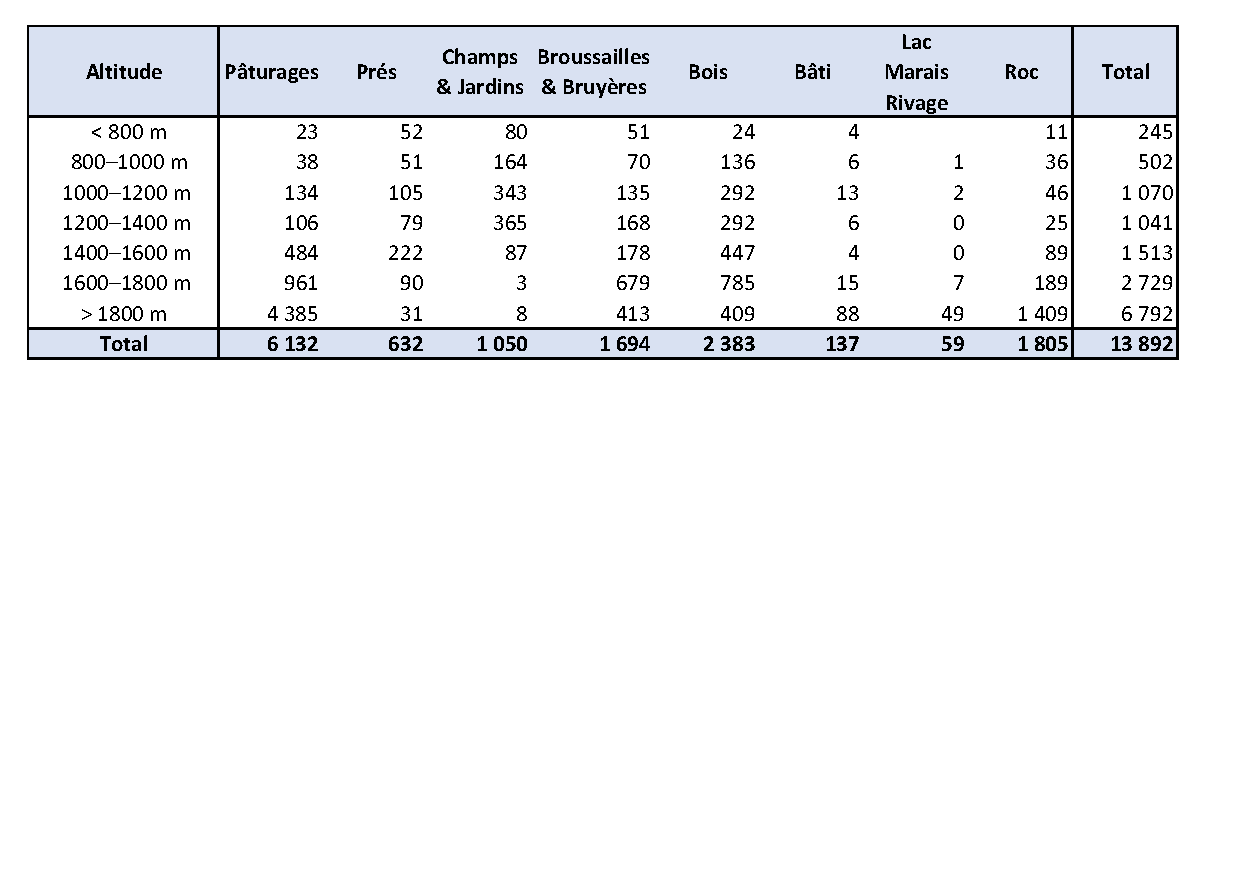
\includegraphics[
		width=\textwidth,
		trim=0cm 8cm 0cm 0cm,
		clip
		]{tables/1 Surface par altitude et OccSol.pdf}
		\tabcaptionindex{tab:occsol-alt}{Occupation du Sol et Altitude : Surface en ha}
	\end{table}
	
	Nous retrouvons par ce tableau l’image d’un territoire très important  composé principalement de pâturage (\texttt{38\%}), de forêts (\texttt{16\%}) de champs et de prés (\texttt{12\%}) et de rocs (\texttt{24\%}). 
	
	La répartition des occupations du sol selon l'altitude fait apparaître une rupture nette aux environs de 1600 mètres.
	
	Sous cette altitude se concentrent la quasi-totalité des champs et jardins ainsi qu'une très forte proportion des prés. Les cultures céréalières et les espaces de production fourragère se développent principalement entre 800 et 1400 mètres, là où les conditions climatiques demeurent les plus favorables.
	



\begin{landscape}
	\thispagestyle{empty}
	
	\begin{figure}[p]
		\centering
		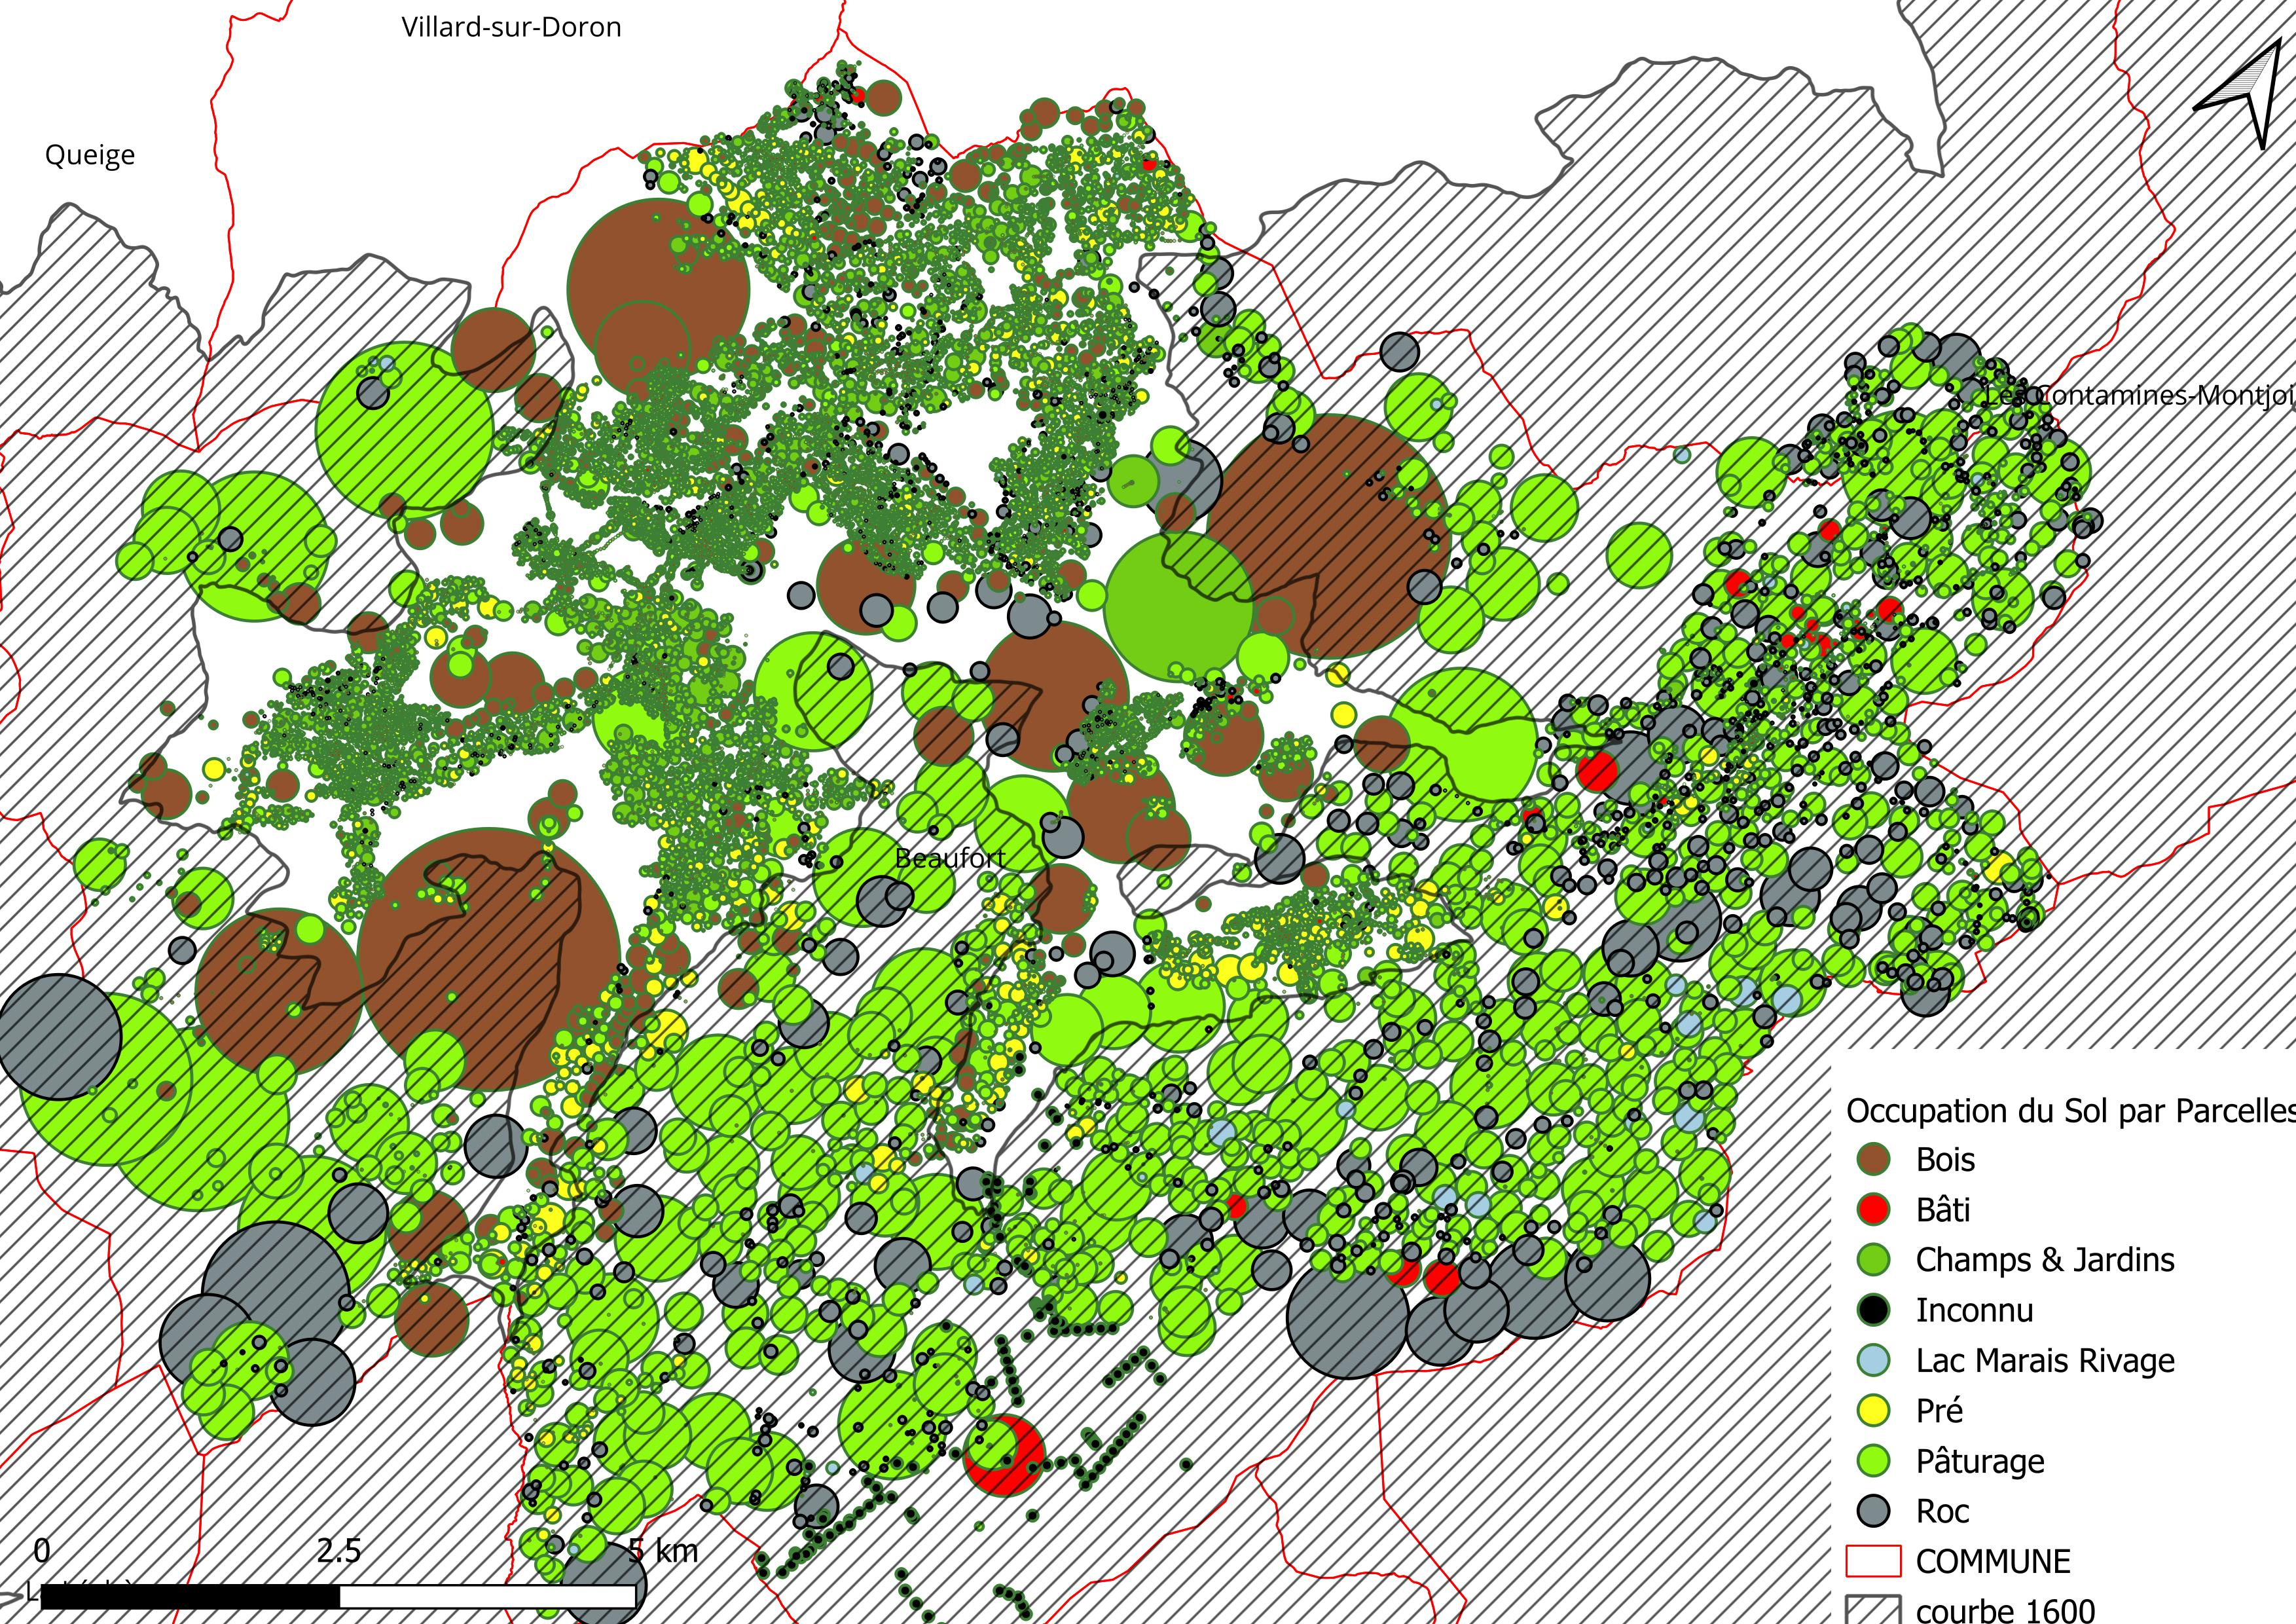
\includegraphics[
		width=\paperwidth,
		height=0.92\paperheight,
		keepaspectratio
		]{figures/3_Carte_OccSol_Parcelle.jpg}
		\caption{Occupation du Sol (la taille du cercle est fonction de la superficie de la parcelle}
		\label{OccSolParc}
		\idxcarte{Fig.~\thefigure{} -- Vue aérienne des Alpes occidentales (Géoportail)}
	\end{figure}
	
\end{landscape}
	À l'inverse, au-dessus de 1600 mètres, les surfaces cultivées deviennent marginales tandis que les pâturages occupent une place prépondérante. Les bois, broussailles et terrains rocheux représentent également une part importante des surfaces recensées. Cette évolution traduit les contraintes imposées par l'altitude mais également l'adaptation des activités humaines aux différents étages de la montagne.
	
	La rupture observée vers 1600 mètres ne correspond toutefois pas à une limite entre un espace occupé et une montagne déserte. Elle marque plutôt le passage entre deux formes complémentaires d'exploitation du territoire : d'une part un espace dominé par les cultures et l'habitat permanent, d'autre part un espace largement consacré aux activités pastorales.
	
\subsection{Une montagne intensément fréquentée}
	
	L'étude du bâti confirme cette interprétation.
	Les parcelles "bâties" sont plus intéressantes à analyser en nombre de parcelles plutôt qu'en superficie.
	
	
	\cartefigure
	{figures/3_Parcelles_Baties.jpg}
	{fig:BatieParc}
	{Parcelles Bâties}
	
Les maisons sont majoritairement concentrées dans les étages inférieurs, particulièrement entre 800 et 1400 mètres d'altitude. Cette répartition correspond à l'implantation des principaux villages et hameaux permanents de la paroisse.

\cartefigure
{figures/3_Parcelles_Baties_zoom.jpg}
{fig:ZoomBati}
{Parcelles Baties : le bourg de Saint-Maxime et Mas environnants}


	
Cependant, les hautes altitudes ne sont nullement dépourvues de constructions. Au-dessus de 1600 mètres, les registres recensent principalement des granges, des greniers, des maisons d'alpage et des masures. Leur présence témoigne d'une occupation saisonnière intense de la montagne.

\begin{table}[htbp]
		\centering
		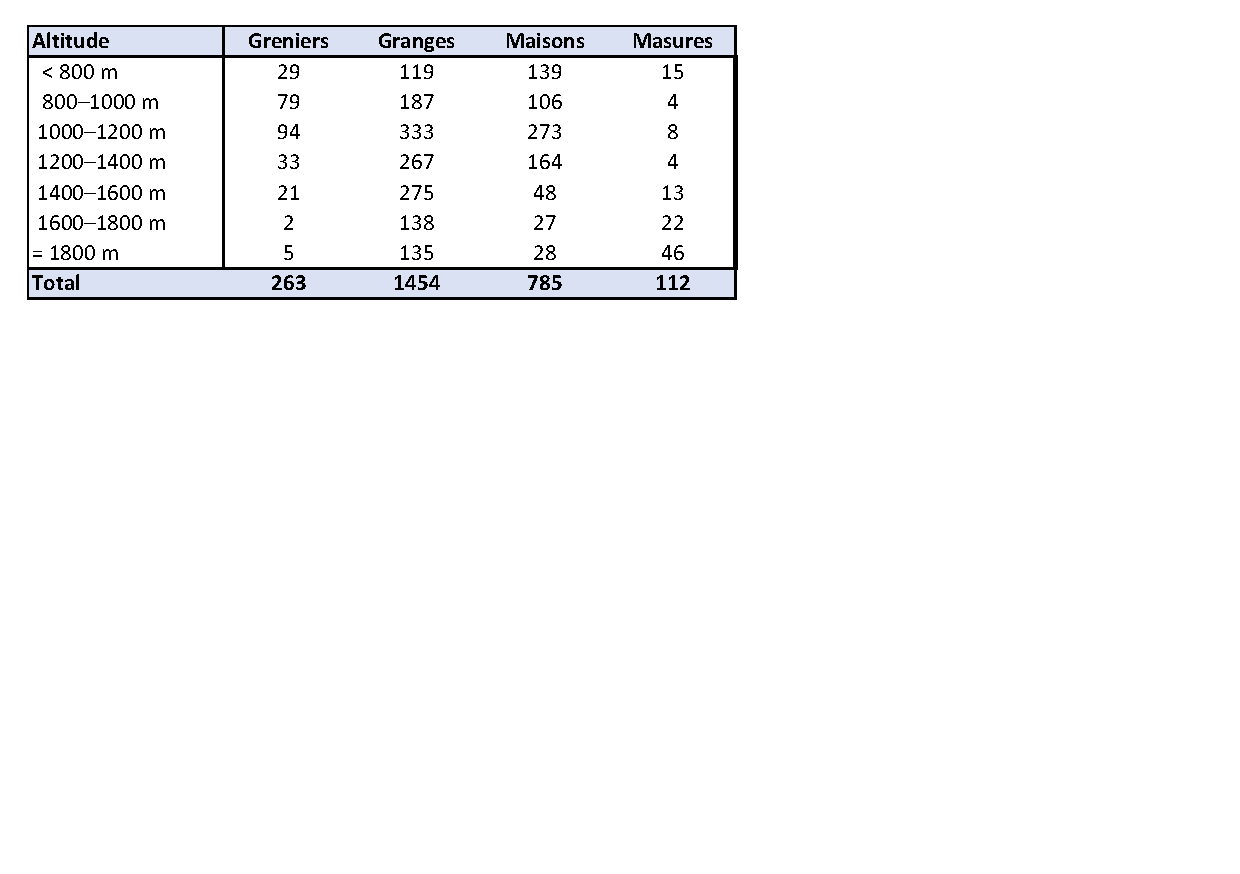
\includegraphics[
		width=\textwidth,
		trim=0cm 9cm 0cm 0cm,
		clip
		]
		{tables/1_Alt_OccSol_Bati.pdf}
		\tabcaptionindex{tab:occsol-bati}{Analyse des Bâtiments (en nb de parcelles)}
\end{table}
	
	

	Cette répartition reflète l'organisation de l'économie beaufortaine. Les troupeaux sont conduits vers les alpages durant la belle saison et la fabrication du fromage s'effectue directement dans les montagnes. Les bâtiments d'altitude constituent ainsi les infrastructures indispensables au fonctionnement du système pastoral : logement temporaire des hommes, abri des animaux, stockage de foin, stockage des produits agricoles et transformation du lait.
	
	L'opposition entre les étages ne doit donc pas être comprise comme une séparation entre espace habité et espace vide, mais comme la coexistence de deux formes d'occupation complémentaires : un habitat permanent concentré dans les basses et moyennes altitudes et un habitat saisonnier étroitement associé à l'exploitation des alpages.
	
	Les actes étudiés par Hélène Viallet montrent que les exploitations beaufortaines mobilisent simultanément plusieurs bâtiments répartis sur plusieurs centaines de mètres de dénivelé, illustrant la pratique des "remues" entre les différents étages de la montagne.\footcite[54--55]{HViallet1993} Cette transhumance verticale fonctionne encore aujourd'hui.
	 

	
\subsection{La question du degré de bonté}
	
	\begin{table}[htbp]
		\centering
		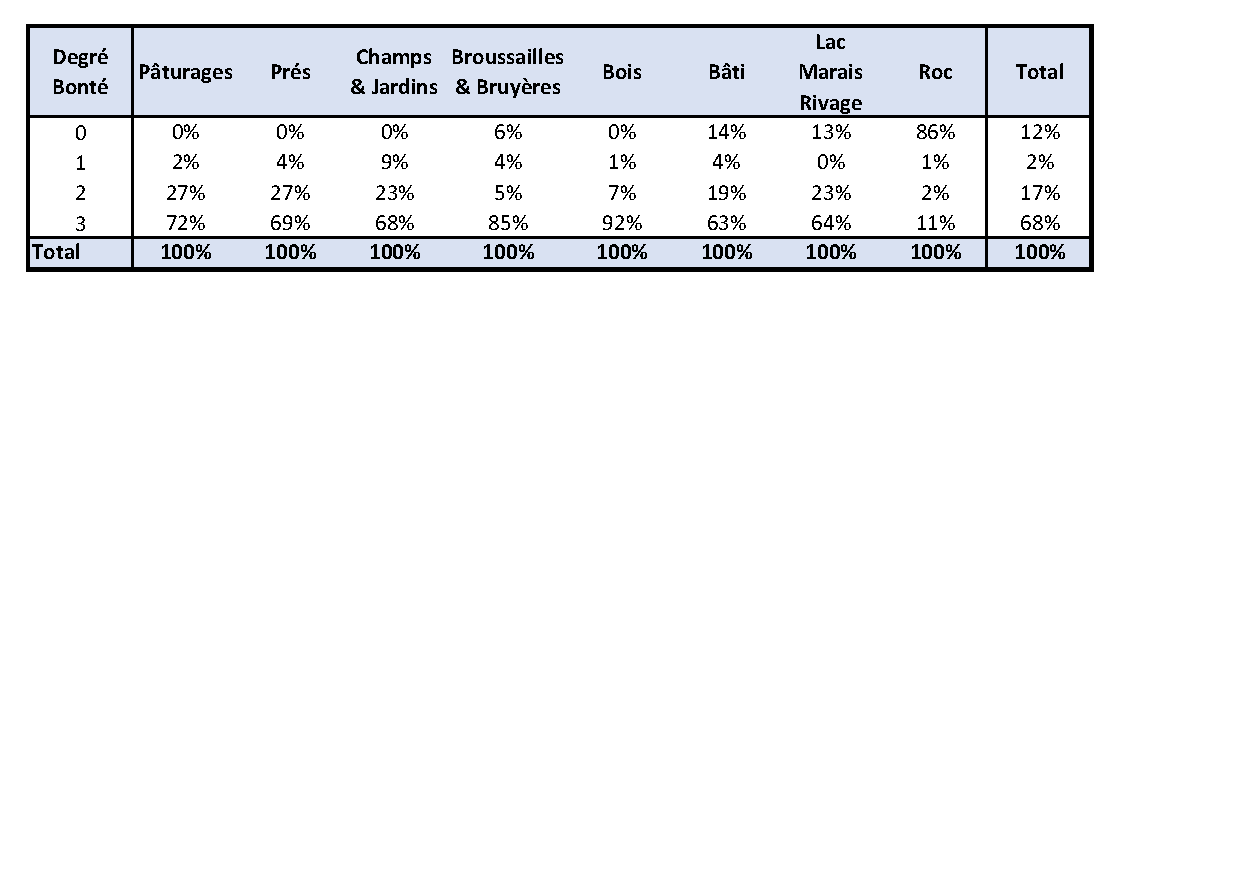
\includegraphics[
		width=\textwidth,
		trim=0cm 10cm 0cm 0cm,
		clip
		]
		{tables/1_OccSol_DB.pdf}
		\tabcaptionindex{tab:occsol-db}{Occupation du Sol par Degré de Bonté (en \% de Surface)}
	\end{table}
	
	
	Attention : de manière contre-intuitive (pour nous, aujourd'hui), si les terrains de nul produit dont bien classé avec un degré de bonté nul, les meilleures terres sont affectées du degré 1, puis 2 pour les terres moyennes, et enfin 3 pour les terres "pauvres". 
	
	Ainsi, plus des 2/3 de la surface de la commune sont en terre "pauvre" et seulement 2\% en terres riches (essentiellement des jardins en fond de vallée).
	
	Cette observation mérite cependant d'être nuancée. Le degré de bonté utilisé dans la fiscalité sarde ne constitue pas une mesure strictement agronomique de la fertilité des sols. Il s'agit avant tout d'un outil d'évaluation fiscale destiné à apprécier la valeur économique des biens afin de répartir l'impôt.
	
	Dans une région où l'élevage et l'exploitation des alpages jouent un rôle déterminant, les estimateurs ont pu attribuer des degrés faibles à des terrains dont l'intérêt économique était important, même lorsque leur aptitude à la culture restait limitée. Un alpage productif pouvait ainsi recevoir une évaluation médiocre puisque non labourable et improductif 8 mois sur 12.
	
	Il faut également tenir compte de la logique de péréquation fiscale mise en œuvre à l'échelle du duché. Afin de maintenir une répartition cohérente de l'impôt entre des communautés aux ressources très différentes, les agents chargés des estimations ont vraisemblablement accordé une attention particulière à la valeur économique des ressources pastorales qui constituaient l'une des principales richesses du Beaufortain mais du fait de l'importance de la surface de la commune aurait pu aboutir à un impôt calculé exagérément élevé.
	
	Les degrés de bonté élevés observés pour les communaux doivent donc être interprétés avec prudence. Ils témoignent probablement davantage de la valeur économique reconnue aux alpages, pâturages et espaces forestiers que d'une qualité agronomique exceptionnelle ou médiocre des sols.
	
\subsection{Conclusion}
	
	L'étude croisée de l'altitude, de l'occupation du sol, du bâti et du statut foncier met en évidence la forte spécialisation verticale du territoire Beaufortain.
	
	Les basses et moyennes altitudes concentrent sur de nombreuses petites parcelles l'habitat permanent, les cultures et les principaux espaces de production fourragère. Les hautes montagnes sont quant à elles dominées par les pâturages, les espaces forestiers et les terrains de parcours indispensables à l'économie pastorale.
	
	Cette organisation ne traduit pas une opposition entre espaces riches et espaces pauvres ni entre territoires occupés et délaissés. Elle révèle au contraire la complémentarité de différents étages de montagne dont chacun remplit une fonction spécifique. Les communaux occupent une place centrale dans ce système en assurant la gestion collective d'une part importante des ressources pastorales et forestières qui fondent la prospérité économique de la communauté.
	
	


\section{Questionnement sur les mas et les patronymes}

	\begin{quote}
	« Gabriel Pérouse écrivait qu’en Savoie, les communautés paysannes sont avant tout des associations de propriétaires, tenant en indivision des biens concédés par un seigneur. C’est absolument vrai en Faucigny, à condition de préciser que les communuitates de hameaux, les plus nombreuses, sont probablement assez souvent, à l’origine, des communautés lignagères. De nombreux hameaux faucignerans ont donc une origine familiale.»\footcite[248]{Carrier2001VieMontagnardeFaucigny}
\end{quote}

Dans son étude sur le Faucigny médiéval, Nicolas Carrier propose que certains mas et communaux puissent trouver leur origine dans d'anciennes exploitations familiales demeurées longtemps indivises. Il écrit ainsi :

\begin{quote}
	« D’où la tentation de penser que les communaux de hameaux, qui sont si nombreux aux XIV\**e et XVe siècles, sont, pour une bonne partie d’entre eux, d’anciennes propriétés familiales restées indéfiniment indivises. [...] Il semble donc bien que les communaux de prises et de mas correspondent à la part des terres de ces exploitations qui n’a jamais été partagée. »\footcite[247]{Carrier2001VieMontagnardeFaucigny}
\end{quote}

Plus loin, l'auteur souligne également que de nombreuses communautés de hameaux pourraient avoir eu une origine lignagère :

\begin{quote}
	« De nombreux hameaux faucignerans ont donc une origine familiale. Ils sont nés et se sont développés parce que des cognats continuaient à voisiner après avoir quitté la cohabitation, et gardaient sur de nombreuses générations une partie de leurs biens en communs, ainsi devenus communia de hameaux. »\footcite[247-248]{Carrier2001VieMontagnardeFaucigny}
\end{quote}

De telles hypothèses soulèvent naturellement la question de savoir si des traces de ces communautés familiales anciennes demeurent perceptibles dans le Beaufortain du XVIIIe siècle. Si certains mas ont effectivement pour origine des groupes de parenté ayant reçu ou défriché collectivement un territoire au Moyen Âge, on peut s'attendre à y retrouver, plusieurs siècles plus tard, une concentration anormalement forte de certains patronymes.

La Mappe Sarde offre la possibilité d'explorer cette question à travers les propriétaires déclarés en 1730. L'objectif n'est pas de démontrer l'existence de telles communautés lignagères, mais de vérifier si leur éventuelle existence médiévale demeure encore perceptible dans la structure de la propriété foncière observée au XVIIIe siècle.

\begin{table}[H]
	\centering
	 \resizebox{0.6\textwidth}{!}{%
	 	
\begin{tabular}{lrrlr}
\toprule
Patronyme & Nb_prop & Surface & Mas & Surface_Mas\\
\midrule
BLANC & 18 & 1203.26 &  & \\
 &  &  & Roniaux & 291.48\\
 &  &  & Traicol & 249.25\\
 &  &  & Lay & 180.02\\
 &  &  & Couecle & 101.6\\
\addlinespace
 &  &  & Borne Et Meralliet & 78.1\\
 &  &  & Val De Treicol & 63.12\\
 &  &  & Planay Voisin De La Grande Combe & 35.23\\
 &  &  & Roselend & 34.21\\
 &  &  & Voniaret & 30.72\\
\addlinespace
DOIX & 22 & 610.05 &  & \\
 &  &  & Berge & 115.72\\
 &  &  & Charmette & 62.54\\
 &  &  & Val & 60.17\\
 &  &  & Bettiere & 52.73\\
\addlinespace
 &  &  & Roniaux & 38.1\\
 &  &  & Gitte & 33.26\\
BOCHET & 29 & 552.13 &  & \\
 &  &  & Lay & 226.79\\
 &  &  & Grande Combe & 177.17\\
\addlinespace
 &  &  & Planay Voisin De La Grande Combe & 38.61\\
GACHET & 26 & 384.89 &  & \\
 &  &  & Gitte & 162.48\\
 &  &  & Sceause & 77.89\\
 &  &  & Roselend & 42.67\\
\addlinespace
 &  &  & Val De Treicol & 42.14\\
VIBERT & 32 & 247.56 &  & \\
 &  &  & Val & 49.57\\
 &  &  & Val De Treicol & 44.37\\
VIALLET & 39 & 231.21 &  & \\
\addlinespace
 &  &  & Cres Denset & 64.31\\
 &  &  & Bouchères & 30.03\\
NEIROUD & 15 & 180.28 &  & \\
 &  &  & Borne Et Meralliet & 58.25\\
 &  &  & Perrosan & 57.43\\
\addlinespace
MOLLIET & 18 & 87.99 &  & \\
 &  &  & Lay & 56.03\\
JOLY & 18 & 78.56 &  & \\
 &  &  & Bettiere & 33.34\\
\bottomrule
\end{tabular}

	}
	\caption{Principaux patronymes et répartition par mas}
	\label{tab:PatronymesMas}
\end{table}

Le tableau présente les patronymes associés à plus de quatorze propriétaires distincts dans l'ensemble de la paroisse (hors « Institution »). Pour chaque patronyme sont indiqués le nombre total de propriétaires correspondants et la surface totale détenue. Ne sont ensuite affichés que les mas dans lesquels ce patronyme possède au moins 30 hectares, avec la surface correspondante.

Le tableau \ref{tab:PatronymesMas} présente ainsi les principaux patronymes de la paroisse et leur répartition foncière entre les différents mas. Si certaines familles semblent particulièrement associées à certains secteurs — les Blanc à Traicol et à Lay, les Doix à Berge ou Charmette, les Viallet à Cres Denset ou Bouchères — aucune n'apparaît véritablement cantonnée à un territoire précis.

\medskip

Au contraire, les principaux patronymes sont présents dans de nombreux mas distincts, parfois éloignés les uns des autres. Cette dispersion géographique traduit une circulation ancienne des patrimoines fonciers, résultant probablement des successions, des alliances matrimoniales, des ventes, des échanges et des recompositions d'indivisions.

Cette observation est particulièrement intéressante au regard des hypothèses formulées pour d'autres régions alpines, où certains auteurs ont proposé une origine lignagère des mas et des communaux. Si certains territoires ont pu être initialement concédés à un groupe familial ou à une communauté de parents, la situation observée à Beaufort en 1730 ne permet plus d'en retrouver clairement la trace à travers la seule répartition des patronymes.

\begin{table}[H]
	\centering
	\resizebox{0.6\textwidth}{!}{%
		
\begin{tabular}{l}
\toprule
\textbf{Gitte} : 1889.6 ha ; 13 patronymes ; 20 propriétaires\\
\hspace{1em}GACHET (1 prop.) : 162.5 ha\\
\hspace{1em}BOUCHAGE (3 prop.) : 143 ha\\
\hspace{1em}DOIX (2 prop.) : 33.3 ha\\
\\
\addlinespace
\textbf{Lay} : 1199.5 ha ; 8 patronymes ; 11 propriétaires\\
\hspace{1em}BOCHET (1 prop.) : 226.8 ha\\
\hspace{1em}LANCHE (2 prop.) : 221.3 ha\\
\hspace{1em}BLANC (3 prop.) : 180 ha\\
\hspace{1em}CORNU (1 prop.) : 151.2 ha\\
\addlinespace
\hspace{1em}MOLLIET (1 prop.) : 56 ha\\
\\
\textbf{Ladray} : 891.8 ha ; 23 patronymes ; 65 propriétaires\\
\hspace{1em}PERRIER (11 prop.) : 56.8 ha\\
\\
\addlinespace
\textbf{Roselend} : 457.3 ha ; 25 patronymes ; 49 propriétaires\\
\hspace{1em}BOUCHAGE (7 prop.) : 78.7 ha\\
\hspace{1em}GACHET (3 prop.) : 42.7 ha\\
\hspace{1em}BLANC (3 prop.) : 34.2 ha\\
\hspace{1em}LANCHE (3 prop.) : 25.5 ha\\
\addlinespace
\\
\textbf{Traverse} : 248 ha ; 21 patronymes ; 43 propriétaires\\
\hspace{1em}DUC (13 prop.) : 27.4 ha\\
\\
\textbf{Val De Treicol} : 213.6 ha ; 6 patronymes ; 10 propriétaires\\
\addlinespace
\hspace{1em}BLANC (3 prop.) : 63.1 ha\\
\hspace{1em}VIBERT (2 prop.) : 44.4 ha\\
\hspace{1em}GACHET (1 prop.) : 42.1 ha\\
\\
\textbf{Val} : 187.4 ha ; 5 patronymes ; 6 propriétaires\\
\addlinespace
\hspace{1em}DOIX (1 prop.) : 60.2 ha\\
\hspace{1em}VIBERT (2 prop.) : 49.6 ha\\
\\
\textbf{Bouchères} : 176.5 ha ; 11 patronymes ; 19 propriétaires\\
\hspace{1em}VIALLET (8 prop.) : 30 ha\\
\addlinespace
\\
\textbf{Cres Denset} : 128.6 ha ; 4 patronymes ; 9 propriétaires\\
\hspace{1em}VIALLET (5 prop.) : 64.3 ha\\
\\
\textbf{Charmette} : 115.5 ha ; 7 patronymes ; 10 propriétaires\\
\addlinespace
\hspace{1em}DOIX (3 prop.) : 62.5 ha\\
\\
\textbf{Leila} : 104.2 ha ; 6 patronymes ; 13 propriétaires\\
\hspace{1em}VIALLET (8 prop.) : 28.9 ha\\
\\
\bottomrule
\end{tabular}

	}
	\caption{Grands mas et principaux patronymes associés}
	\label{tab:MasPatronymes}
\end{table}

Le tableau \ref{tab:MasPatronymes} recense les mas de plus de 100 hectares et indique, pour chacun d'eux, sa surface totale, le nombre de patronymes et le nombre de propriétaires distincts (hors « Institution »). Seuls sont retenus les patronymes comptant au moins dix propriétaires dans l'ensemble de la paroisse et possédant au moins 20 hectares dans le mas considéré. Pour chaque patronyme est également indiqué le nombre de propriétaires distincts concernés dans le mas.

Ce deuxième tableau  aborde la question sous l'angle inverse du précédent en partant des plus grands mas de la paroisse. Si l'hypothèse d'une origine familiale des mas demeurait encore visible au XVIIIe siècle, on pourrait s'attendre à observer, dans les grands territoires, une forte concentration de propriétaires portant un même patronyme.

Or les résultats obtenus montrent généralement une situation beaucoup plus complexe. Les grands mas les plus étendus, tels que la Gitte, Roselend, Ladray ou Traverse, rassemblent un nombre élevé de patronymes et de propriétaires distincts. Même lorsque certains noms apparaissent plus fréquemment que d'autres, ils ne représentent qu'une fraction limitée des ayants droit.

Quelques exceptions existent, notamment à Cres Denset, Charmette ou dans le Val de Treicol, où certains patronymes semblent plus fortement représentés. Toutefois, ces cas demeurent isolés et ne suffisent pas à faire apparaître une organisation générale fondée sur des groupes familiaux identifiables.

Ainsi, l'étude des patronymes ne permet pas de mettre en évidence, dans le Beaufortain de 1730, la survivance manifeste de communautés lignagères associées à un mas particulier. Si de telles structures ont existé au Moyen Âge, plusieurs siècles de transmissions successorales, de mariages, de ventes et de recompositions foncières semblent avoir largement effacé leur lisibilité. Les grands mas apparaissent désormais comme des ensembles fonciers composites associant de nombreux lignages plutôt que comme les territoires propres à une famille ou à un groupe de parenté.

En guise de conclusion sur les Mas, il semble que les arpenteurs et géomètres aient simplement transcrit en Mas des territoires tels que les habitants les appelaient, et les appellent encore aujourd'hui : des zones liées à des hameaux (Curtillet, Le Bersend, Les Outards (Autard et Houtard), La Pierre... ) ou des zones qui portent des noms de sites ou de vallées (vallon de la Gite, de Roselend, de Traicol, plateau des Berges, du Plan de la Laie, col de la Bathie, la Grande Combe).\footnote{Les toponymes et appellations utilisés ici correspondent aux dénominations contemporaines.}

\section{Les propriétaires par statut}

\subsection{Les Communs : une propriété essentiellement pastorale}


L'analyse des biens communaux révèle leur forte concentration dans les étages supérieurs de la montagne.

\begin{table}[htbp]
	\centering
	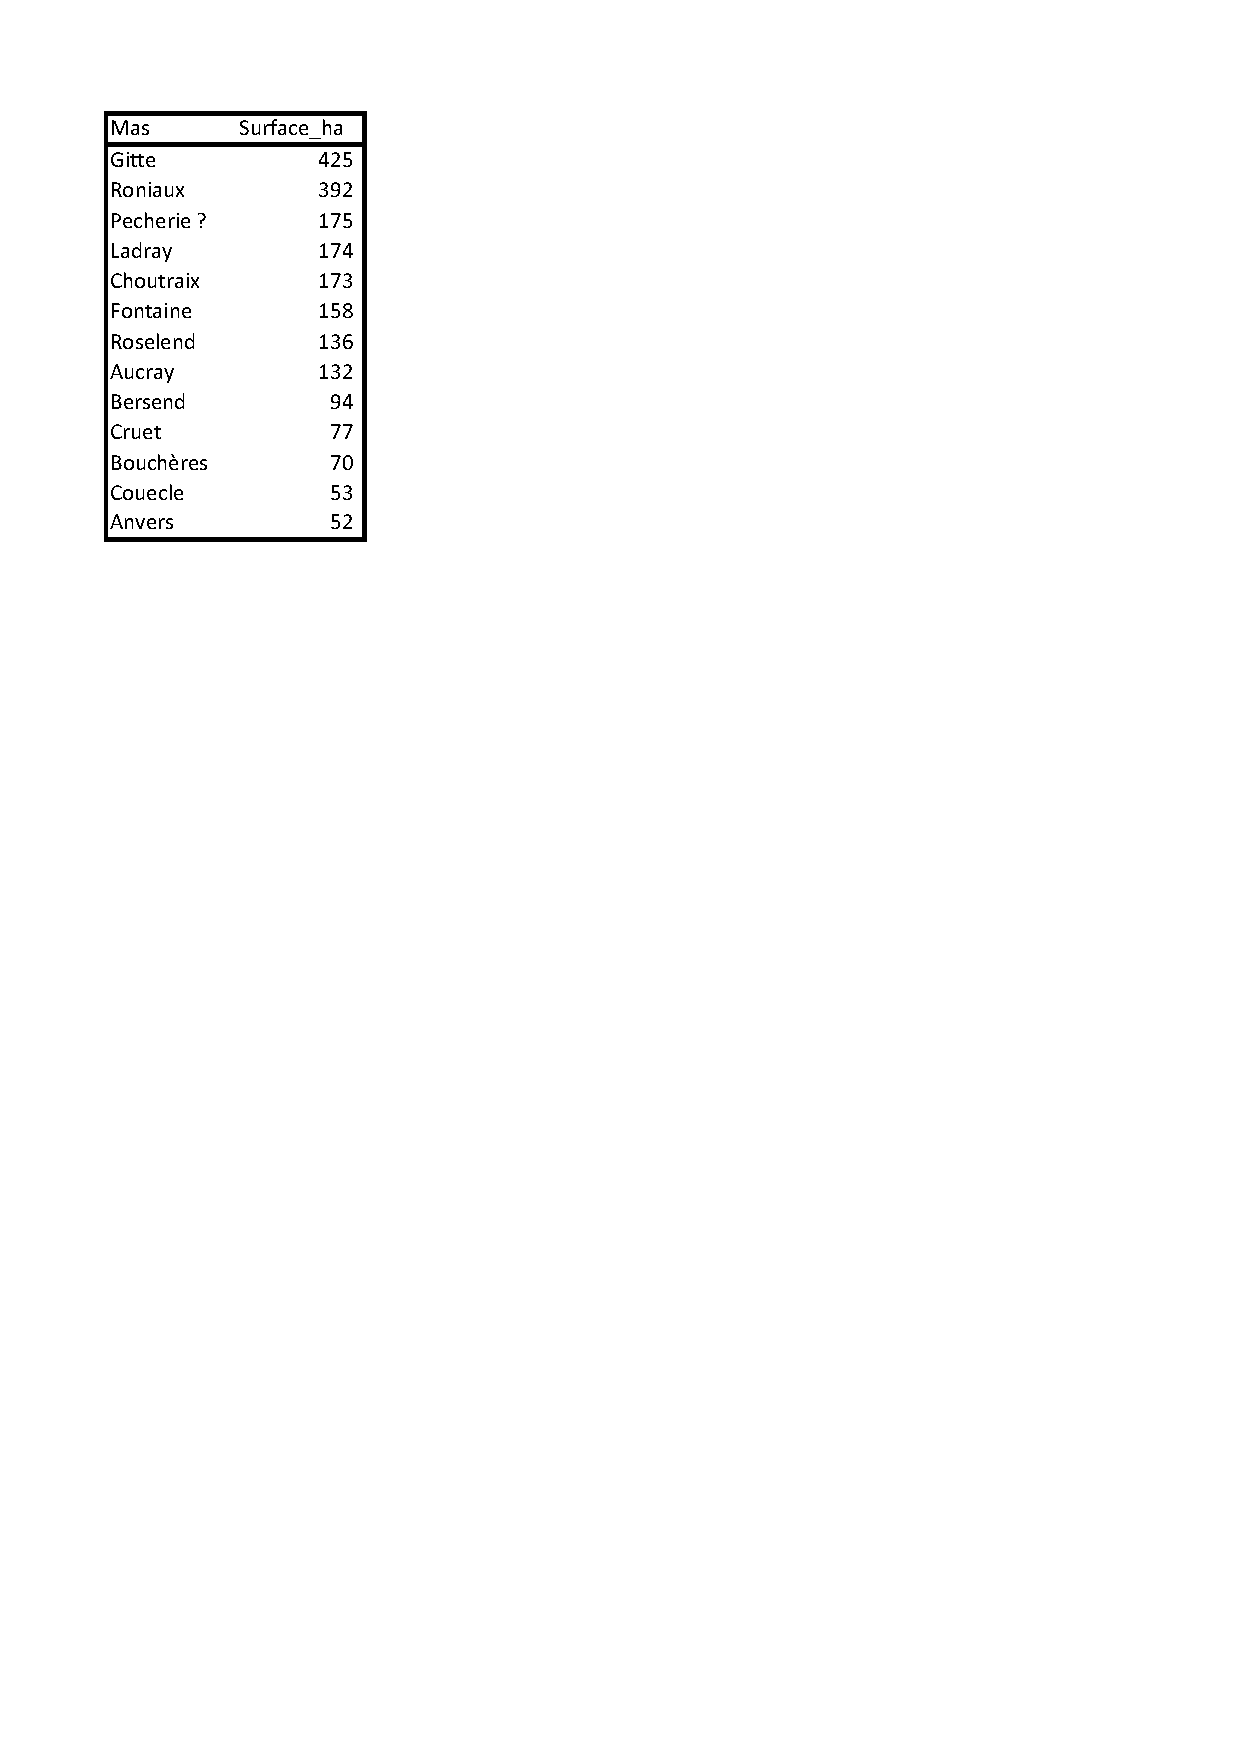
\includegraphics[
	width=\textwidth,
	trim=0cm 20cm 0cm 1.9cm,
	clip
	]
	{tables/3_CommunPaturageMas.pdf}
	\tabcaptionindex{tab:SurfCommun}{Liste des mas qui possèdent de vaste pâturages communs}
\end{table}

Les Communs représentent 6.620ha soient 47\% de la superficie de la commune.
\\
70\% de ces 6,620ha se situent à plus de 1600m d'altitude dont 2,067ha sont des pâturages.
Si l'on considère les pâturages de communs par Mas, nous pouvons constater qu'il existe encore de grand ensemble de pâturage disponible pour la communauté :
\begin{table}[htbp]
	\centering
	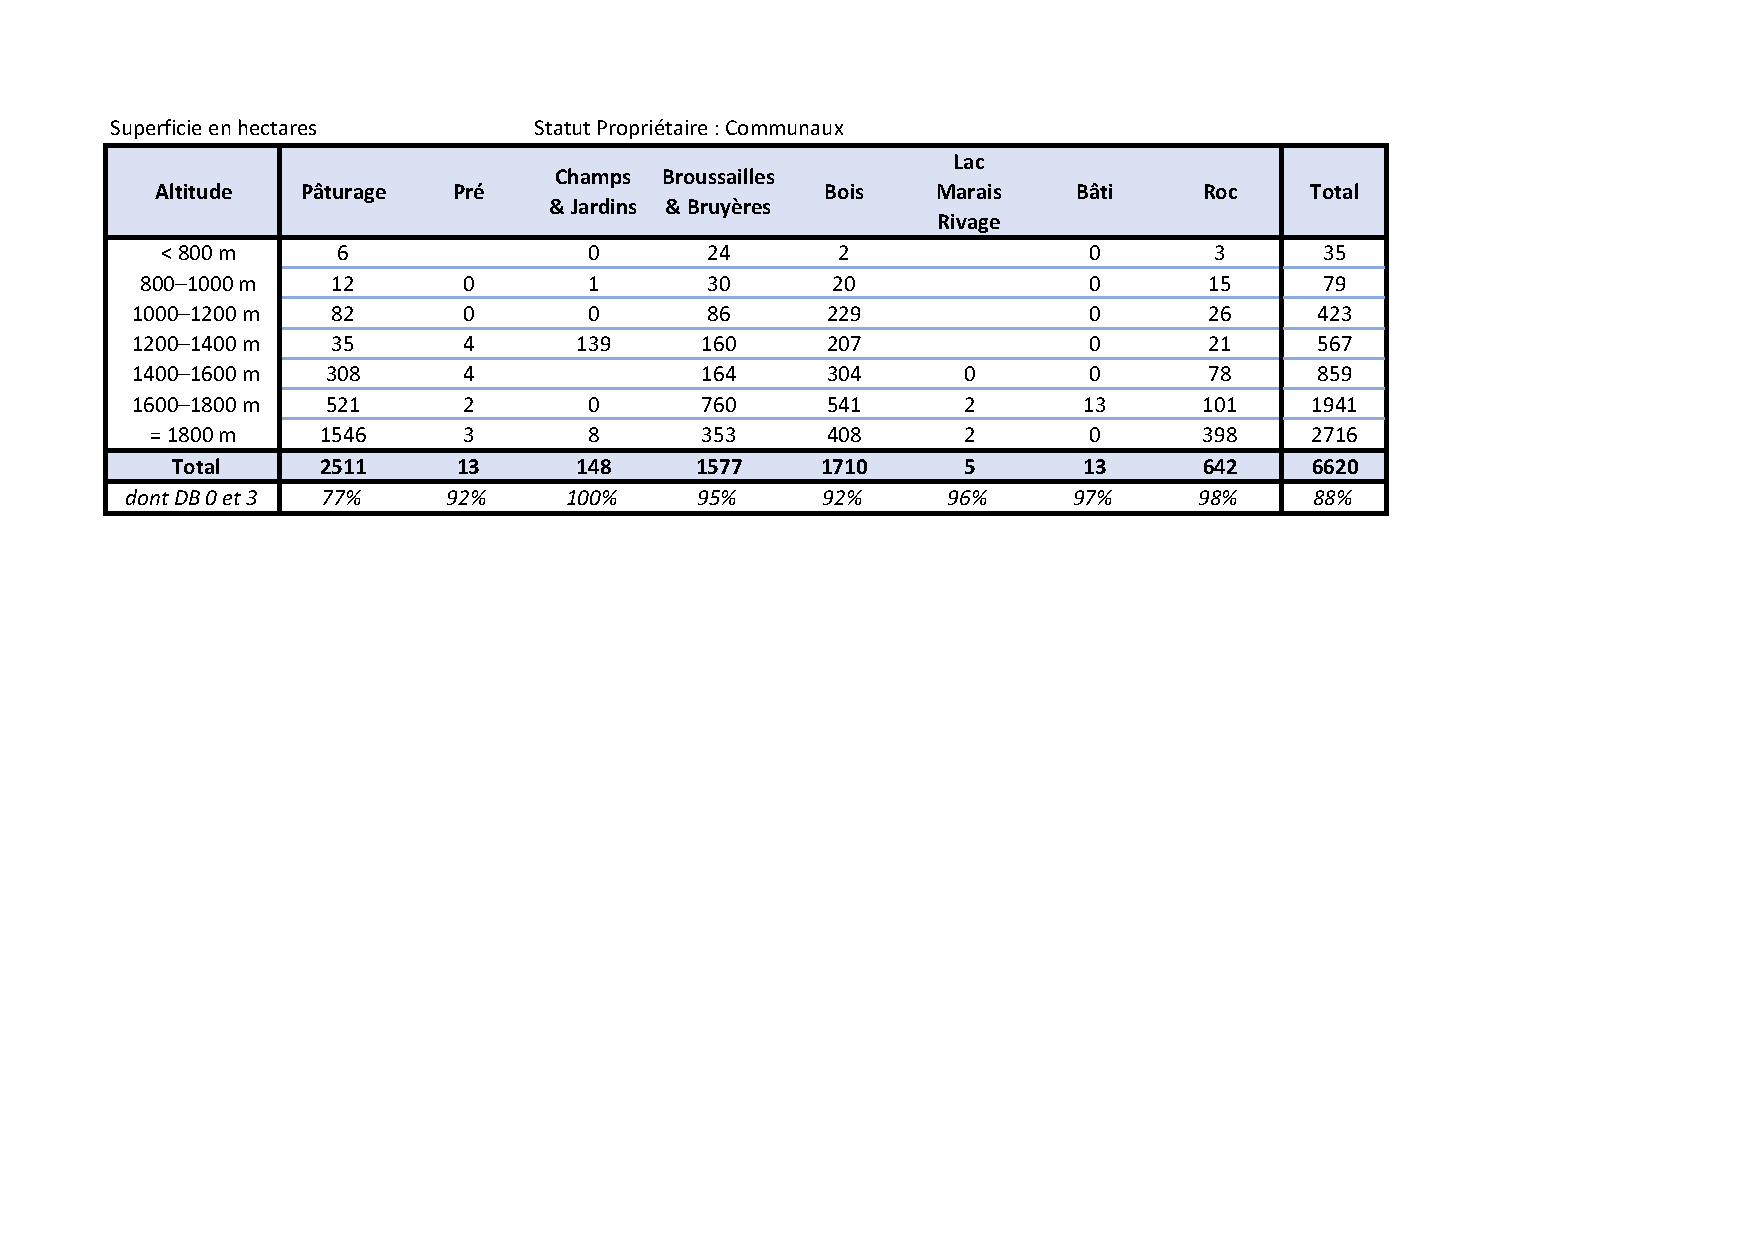
\includegraphics[
	width=\textwidth,
	trim=0cm 12cm 0cm 2cm,
	clip
	]
	{tables/1_Superf_Communaux.pdf}
	\tabcaptionindex{tab:occsol_Alt}{Superficie des Communs par Altitude et Occupation du Sol}
\end{table}

Certes nous ne savons pas combien sont ascencés à des particuliers, mais on peut tout de même questionner l'idée que tous les meilleurs grands pâturages soient accaparés par de riches particuliers (notables ou pas).

Les broussailles et bruyères ainsi que les bois sont aussi très importants y compris dans les étages intermédiaires (entre 1000 et 1600m d'altitude) et ces terrains restent essentiels pour la subsistance de la population pauvre, ayant besoin de bois de chauffage ou d'œuvre (le bâti est essentiellement en bois) ainsi que pour faire paître moutons et chèvres.
Les communaux sont donc composés principalement de pâturages, de bois, de broussailles et de terrains rocheux. À l'inverse, ils comprennent très peu de champs, de prés ou de bâtiments.




\begin{landscape}
	\thispagestyle{empty}
	
	\begin{figure}[p]
		\centering
		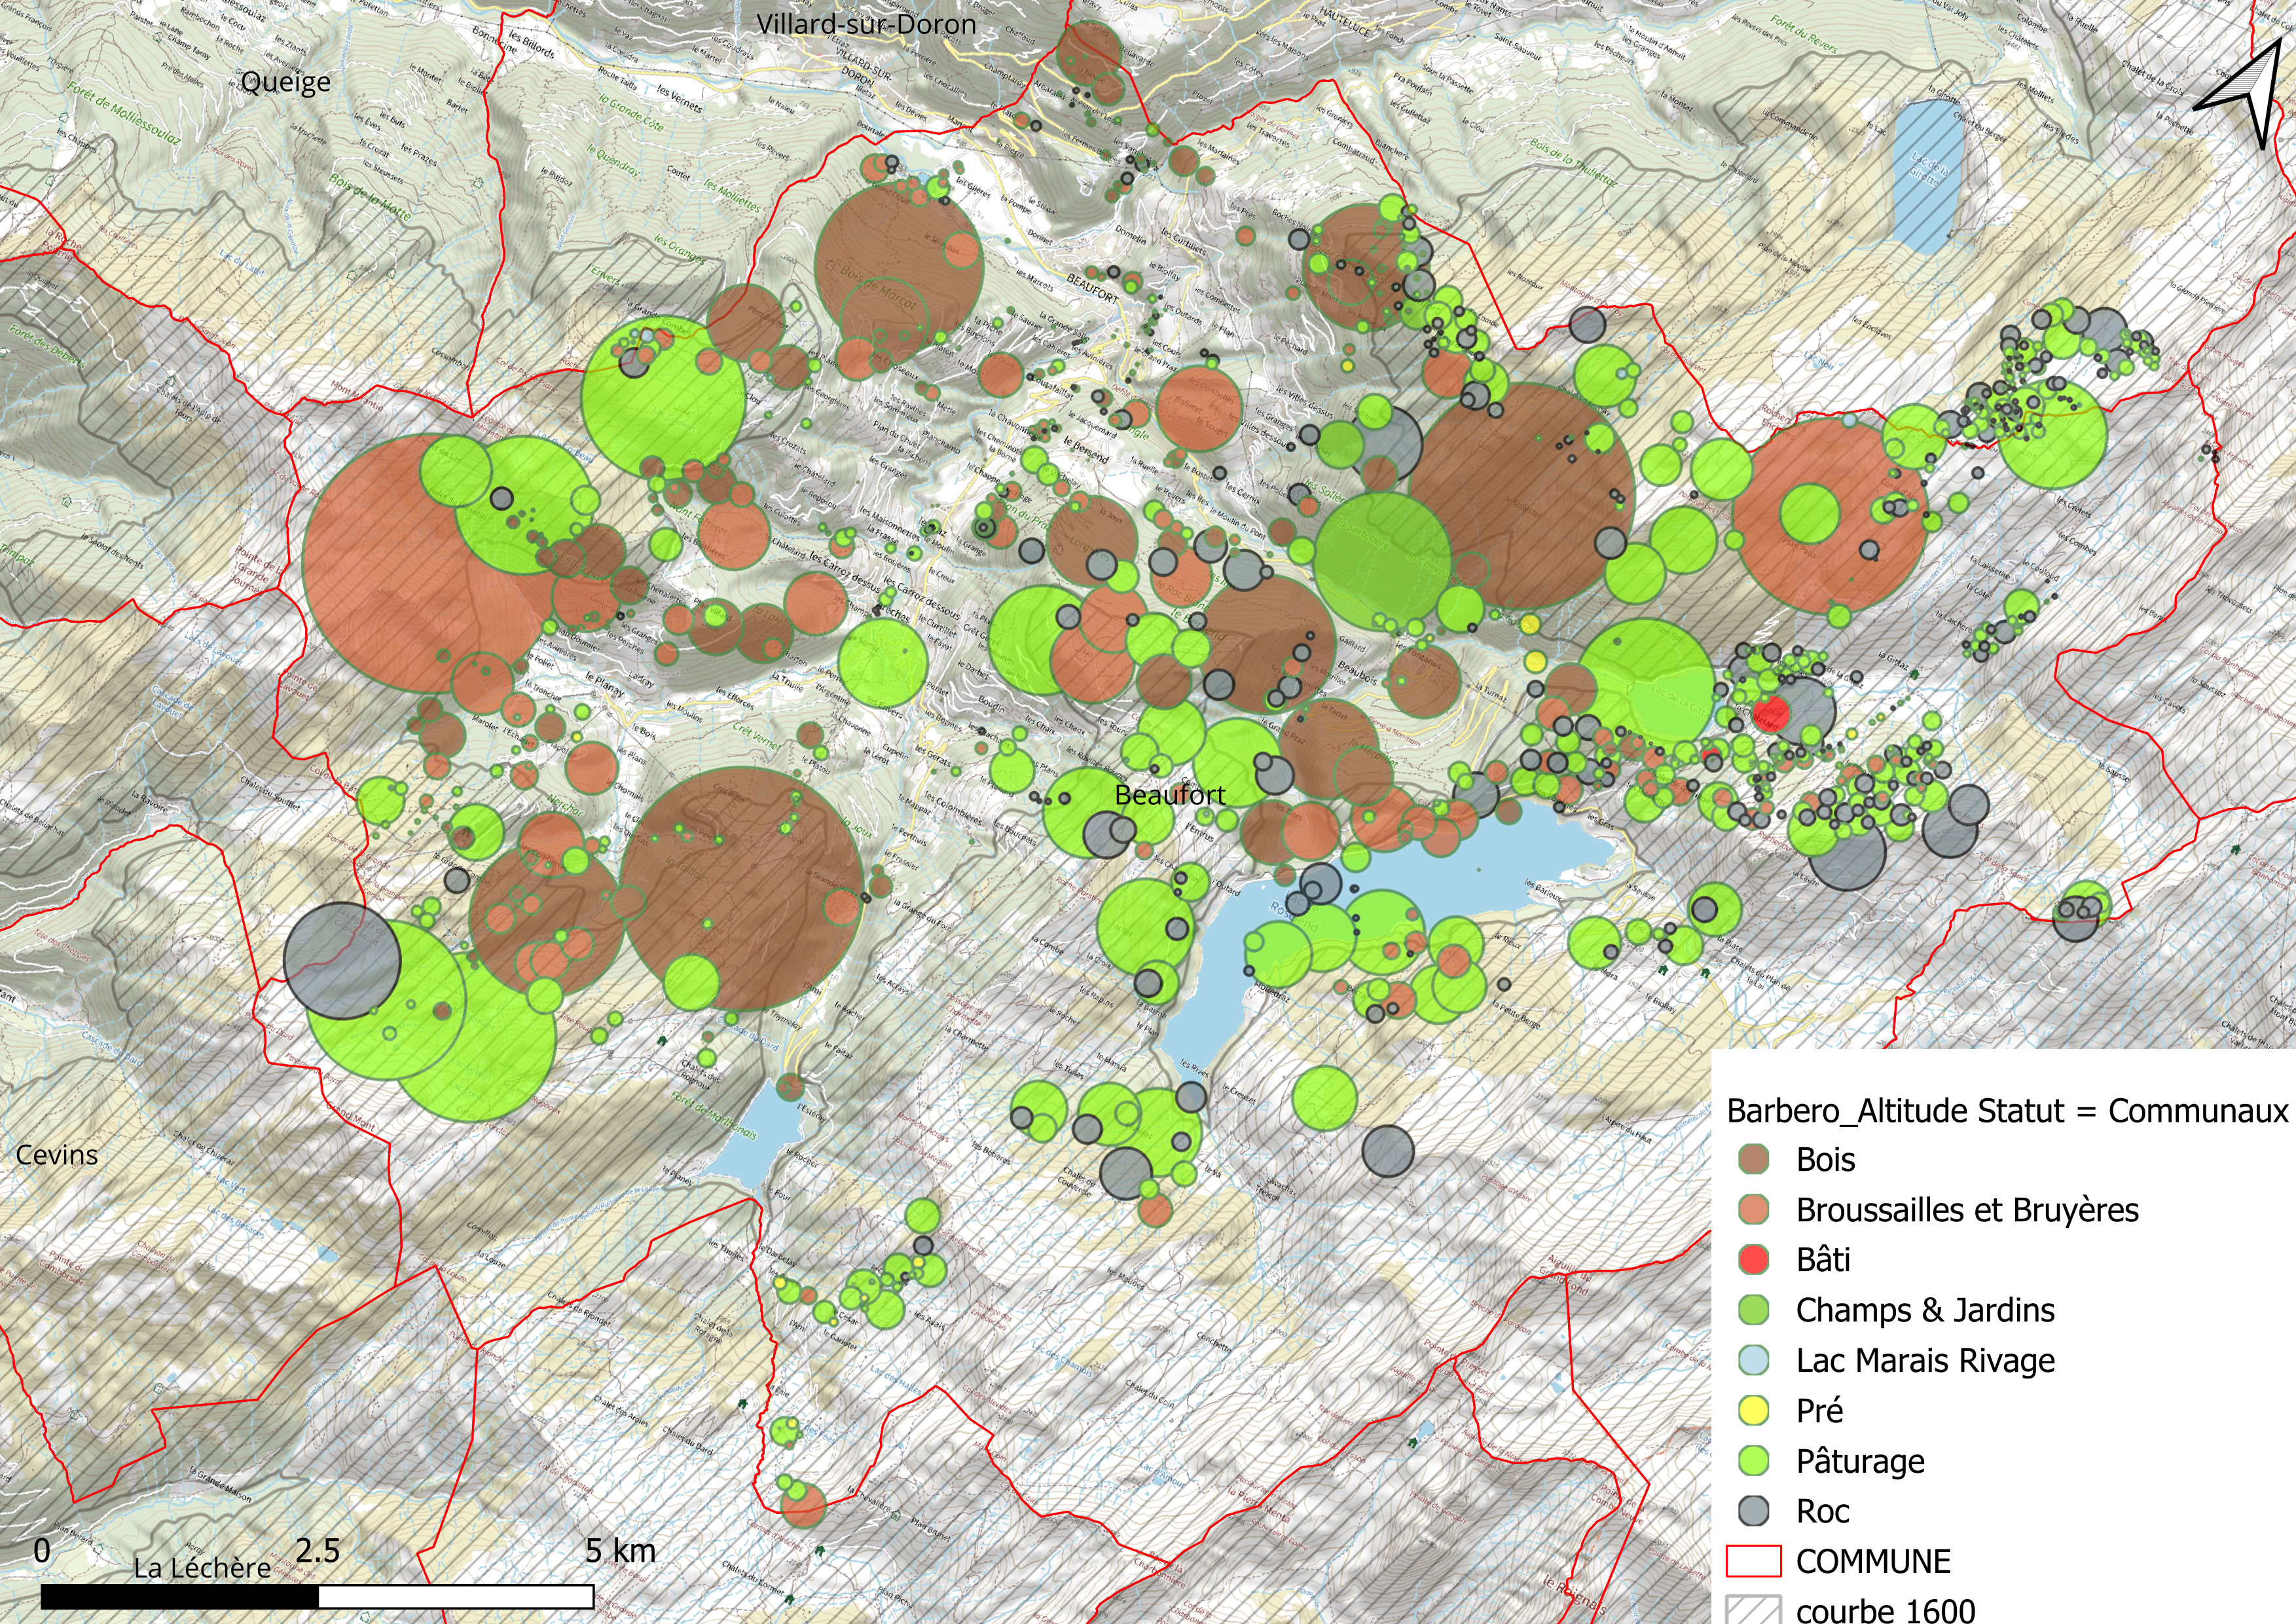
\includegraphics[
		width=\linewidth
		]{figures/3 Carte des Communaux.jpg}
		\caption{Carte des Communs par Occupation du Sol}
		\label{CommunsOccSol}
		\idxcarte{Fig.~\thefigure{} -- Carte des Communs par Occupation du Sol}
	\end{figure}
	
\end{landscape}

\begin{quote}
	« À partir du XIVe siècle, là et seulement là où est passé le mouvement des franchises et des albergements, les eaux, les forêts, les pâturages exploités par les paysans sont désormais reconnus comme des communia, c’est-à-dire des communs. Les communautés en détiennent la propriété utile ce qui inclut le droit d’accès, plus ou moins exclusif, et le droit de police, c’est-à-dire la faculté de réglementer l’exploitation de ces espaces et de réprimer le manquement à ces règles. En Savoie, la communauté paroissiale apparaît comme le cadre naturel de la possession et de la gestion de ces droits. [...] En Savoie, la gestion de l’espace commun est l’affaire de deux institutions qui peuvent agir de manière indépendante ou complémentaire, à savoir la communauté d’habitants et ce que l’on appelle ici les pareries ou, plus couramment, les consortages. […]	En Savoie, la communitas prend donc la paroisse pour cadre exclusif. À tel point qu’au XIVe et au XVe siècle, une communauté de quartier ou de village particulièrement affirmée, va tout faire pour obtenir le statut paroissial, exigeant de son évêque l’érection de la modeste chapelle de hameau en église de plein droit, ou tout au moins en église filiale, dotée d’un cimetière et de fonds baptismaux. La Giettaz, jusque-là quartier de la paroisse de Flumet, devient paroisse annexe en 1390 ; Morzine, quartier de Saint-Jean-d’Aulps, en 1499 ; Morillon »
	\footcite[85]{Mouthon2016}
\end{quote}

On peut imaginer que les nombreuses tentatives du hameau d'Arêches à l'époque moderne, pour obtenir le statut de paroisse distincte de celle de Saint-Maxime ait pour motivation non-exprimée la volonté de se réserver l'usage de "ses" communs.

\begin{quote}
	« Or ce sont ces collectivités, à l’organisation encore incertaine, qui, à la fin du Moyen Âge, se sont vu reconnaître ou confirmer le contrôle des « choses de personne » (\textit{res nullius}) situées sur leur territoire. Lors de l’albergement ou par l’octroi des franchises, le seigneur cède la propriété utile sur les cours d’eau, les forêts, les alpages. Il conserve seulement le droit dit « éminent » ou encore la « directe » dont le cens en argent payé chaque année par la communauté constitue la reconnaissance à la fois symbolique et monétaire. »
	\footcite[86]{Mouthon2016}
\end{quote}


L'occupation du Sol "Roc" est de manière logique très improductive (degré de bonté 0 à 85\%) et cela correspond le plus souvent aux sommets rocailleux des montagnes (1/4 des Roc sont au-dessus de 1800m). En revanche ce qui est moins évident c'est de découvrir grâce à la Mappe que ces sommets inaccessibles et improductifs ne sont pas majoritairement communs : 
Sur les 1,544ha de rochers improductifs (Statut : 'Roc' et DB=0) seuls 525ha appartiennent aux Communs (soit un tiers seulement). 
On peut comprendre que la noblesse puisse avoir conservé depuis le Moyen-Ages des terres historiquement nobles mais il n'y a que 59 ha dans ce cas.
La majorité des rochers improductifs (959ha soit 62\%) est possédée par les particuliers (communiers ou bourgeois). Il serait tentant de vouloir chercher un historique très ancien de cette privatisation des sommets; cependant lors de l'étude que nous avons faite plus loin sur les ventes de communs lors des affranchissements nous y retrouvons concernées 87 parcelles de rochers improductifs. L'explication doit être plus simple et moins historique.cf. chapitre \ref{sec:Affranchissements}\nameref{sec:Affranchissements}

\begin{table}[htbp]
	\centering
	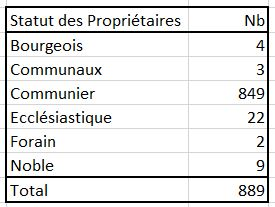
\includegraphics[width=0.5\textwidth]{tables/1 Propriétaires par Statut.JPG}
	\tabcaptionindex{tab:PropStatut}{répartition du nombre de propriétaire par statut}
\end{table}

Il y a trois "propriétaires" sous le statut "Communaux" : "La communauté pour l'usage commun", "La communauté possésdés particulièrement" et petite curiosité : "Les communiers de la communauté de Granier, province de Tarentaise" (48ha de pâturages appartiennent à la paroisse voisine de Granier et ils le sont toujours aujourd'hui).


	
Avant de commercer l’exploration de la propriété des alpages, nous allons essayer de comprendre la propriété dans l’ensemble de Beaufort :
	


	
	
\subsection{Propriétaires déclarés « Ecclésiastique}
	
	Les propriétés ecclésiastiques sont quasi inexistantes (8 ha) et les parcelles sont en grande majorité du bâti (église, chapelles…) et des structures attenante (jardin, cour, cimetière…). Aucun grand propriétaire terrien ecclésiastique, pas de communauté religieuse, ni de biens appartenant à un monastère ou au diocèse de Moutier.

	La liste des 22 propriétaires ecclésiastiques est la suivante :
	
	\begin{itemize}
		\item La Cure de Beaufort
		\item Chapelle du Bersend
		\item Chapelle des Pénitents du Saint-Sacrement
		\item Chapelle d'Arêches
		\item Chapelle de Notre-Dame de Pitié
		\item Chapelle de la Portelaz
		\item Chapelle de la Pierre
		\item Chapelle de Roselend
		\item Chapelle à la Dray
		\item Chapelle de la Frasse
		\item Chapelle des Curtillets
		\item Chapelle des Houtards
		\item Chapelle des Villes-Dessus
		\item Chapelle des Villes-Dessous
		\item Chapelle de la Gitte
		\item Chapelle des Chornets
		\item Chapelle du Mont
		\item Les Révérends Cordeliers de Sainte-Marie-Égyptienne de Chambéry
	\end{itemize}
	
	Les Cordeliers de Chambéry sont la seule communauté religieuse externe et elle ne possède que deux masures avec pré et jardin.
	La présence religieuse est importante au vu du nombre de chapelles mais cela reste cohérent par rapport à la superficie de la commune, la dispersion de l’habitat et les difficultés de se rendre à l’église de Saint-Maxime en hiver.
	
	En revanche 8 prêtres sont propriétaires (seuls ou en indivision), mais sont déclarés comme "communier". Cela ne signifie pas forcément qu'ils exercent sur la paroisse, mais leur patronyme est commun dans la paroisse et on sait que les habitants de Saint-Maxime ont obtenu depuis leMoyen Âge le droit de choisir leurs prêtres.
	
	Ce qui est le cas du propriétaire "communier" : "Rvd LANCHE curé de Beaufort" élu par les paroissiens en 1717.
	
	
	\subsection{Propriétaires déclarés « Noble »}
	
	Les propriétaires nobles sont aussi relativement anecdotiques :
	
	\begin{table}[htbp]
		\centering
		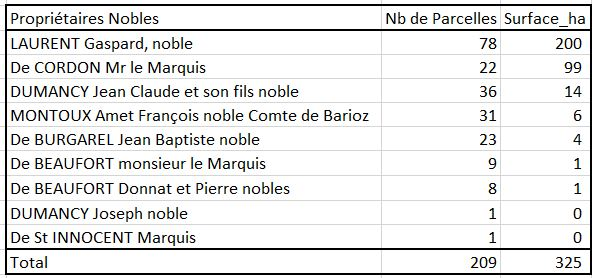
\includegraphics[width=0.7\textwidth]{tables/1 Prop Nobles.JPG}
		\tabcaptionindex{tab:PropNoble}{Liste des propriétaires nobles}
	\end{table}
	

	Le Marquis de Beaufort (dont le premier titre est Marquis de Fleury) ne possède qu’un hectare alors qu’il détient la plupart des droits féodaux sur le mandement de Beaufort.
	
	Gaspard LAURENT(200ha) est un propriétaire important, mais il ne semble pas qu’il s’agisse de terres associées à un historique féodal. 

	Le Marquis de Cordon (99ha) est le seul noble possédant des terres de manière significative ainsi que des droits féodaux sur la commune, sans doute parvenu dans sa famille par alliance ou héritage. Cependant Hélène Viallet signale qu’il est propriétaire d’un alpage de 60 vaches vendu en 1780 \footcite[102]{HViallet1993} mais elle n’en fait pas état dans le cadastre de 1607 ni dans celui de 1645.
	\footnote{François Joseph Sallier de La Tour (1706 - 1799), Marquis de Cordon ; ADS -208 Edépôt 286 Fief de la dame de Saint-Sulpice et du marquis de Cordon. – Etat estimatif de la rente et fief que la comtesse d'Ugine, épouse du seigneur de Saint-Sulpice, a éteint et aboli en faveur des communautés du Villard et Saint-Maxime de Beaufort (1773). Répartition du prix du fief entre les communautés, quittance (1779-1780). Etat de la rente féodale appartenant au marquis de Cordon (1782)} : .
	
	Nous sommes donc loin d’une propriété issue de la féodalité tardive, avec de grands propriétaires fonciers nobles desquels dépendent de nombreux fermiers.
	
	En revanche, concernant le marquis de Cordon et Gaspard Laurent, il est possible qu’il s’agisse d’acquisitions de type  investissement dans les alpages, en parallèle de celles des notaires suite à l’introduction de la fabrication du gruyère dans le Beaufortain.
	
	\begin{quote}
		« Au milieu du XVIe siècle, un quart des nobles tient du bétail, contre 80 \% pour l’ensemble de la population. Ce taux n’est pas négligeable et il atteint 40 \% dans les paroisses rurales. On a même recensé huit feux nobiliaires déclarés pauvres ou misérables. Pauvre ou pas, un noble conserve son rang et ses privilèges, même lorsqu’il travaille la terre ou élève quelques bêtes ; ce n’est pas une activité de dérogeance, à la différence du notariat, du commerce et des arts mécaniques. [...] Quant à la fonction de châtelain, nous l’avons vu, elle a complètement perdu de son prestige au milieu du XVIe siècle et on ne compte que cinq châtelains nobles dont un seul participant aux dénombrements, celui de Rumilly. »
		\footcite[142]{Gachet2011GabelleSel1561}
	\end{quote}
	

	\subsection{Propriétaires déclarés « Bourgeois » ou « Forain »}
	
	Remarque: les forains (du latin foris, « dehors ») sont des propriétaires demeurant dans une autre paroisse, ils sont étranger à la communauté.
	
	\begin{table}[htbp]
		\centering
		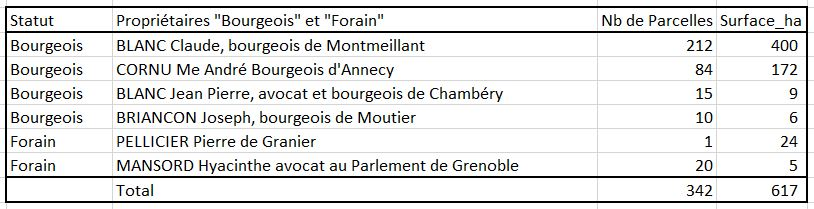
\includegraphics[width=0.7\textwidth]{tables/1 Prop Bourgeois et Forains.JPG}
		\tabcaptionindex{tab:PropBourg}{Liste des propriétaires "bourgeois" et "forains"}
	\end{table}
	
	
	Nous y trouvons en particulier un notaire et deux avocats.
	Nous investiguerons sur le plus gros propriétaire, Claude BLANC, bourgeois de Montmeillant (aujourd’hui Montmelian à côté de Chambéry), il est né, marié et mort à Beaufort, et il est probable que son statut de Bourgeois de Montmeillant soit une volonté de marquer sa notabilité associée à une résidence (hivernale?) proche de la capitale administrative qu'est Chambéry. Son cousin Jean-Pierre Blanc est aussi 'Bourgeois' (de Chambéry) et avocat. Nous y reviendrons lorsque nous étudierons le cas de la famille BLANC.

	Nous avons donc 4 particuliers hors des communiers qui sont de gros propriétaires : deux nobles et deux bourgeois totalisants à eux quatre :1 179ha (soit \texttt{8\%} de la surface de la commune). C'est important, cela les démarque du reste de la population mais cela ne fait pas non plus une domination foncière écrasante des quelques-uns sur le reste des communiers.
	\\
	A l'inverse, les autres notaires de Saint-Maxime ne sont pas "Bourgeois". Ce statut est sans doute significatif fiscalement mais pas pour l'analyse du territoire de Beaufort.
	
	
	
	\subsection{Propriétaires déclarés « Communiers»}
	
	Les communs et les communiers se répartissent à quasi- égalité le reste du foncier (6,620ha pour les communs et 6,016ha pour les communiers) .
	
	\begin{table}[htbp]
		\centering
		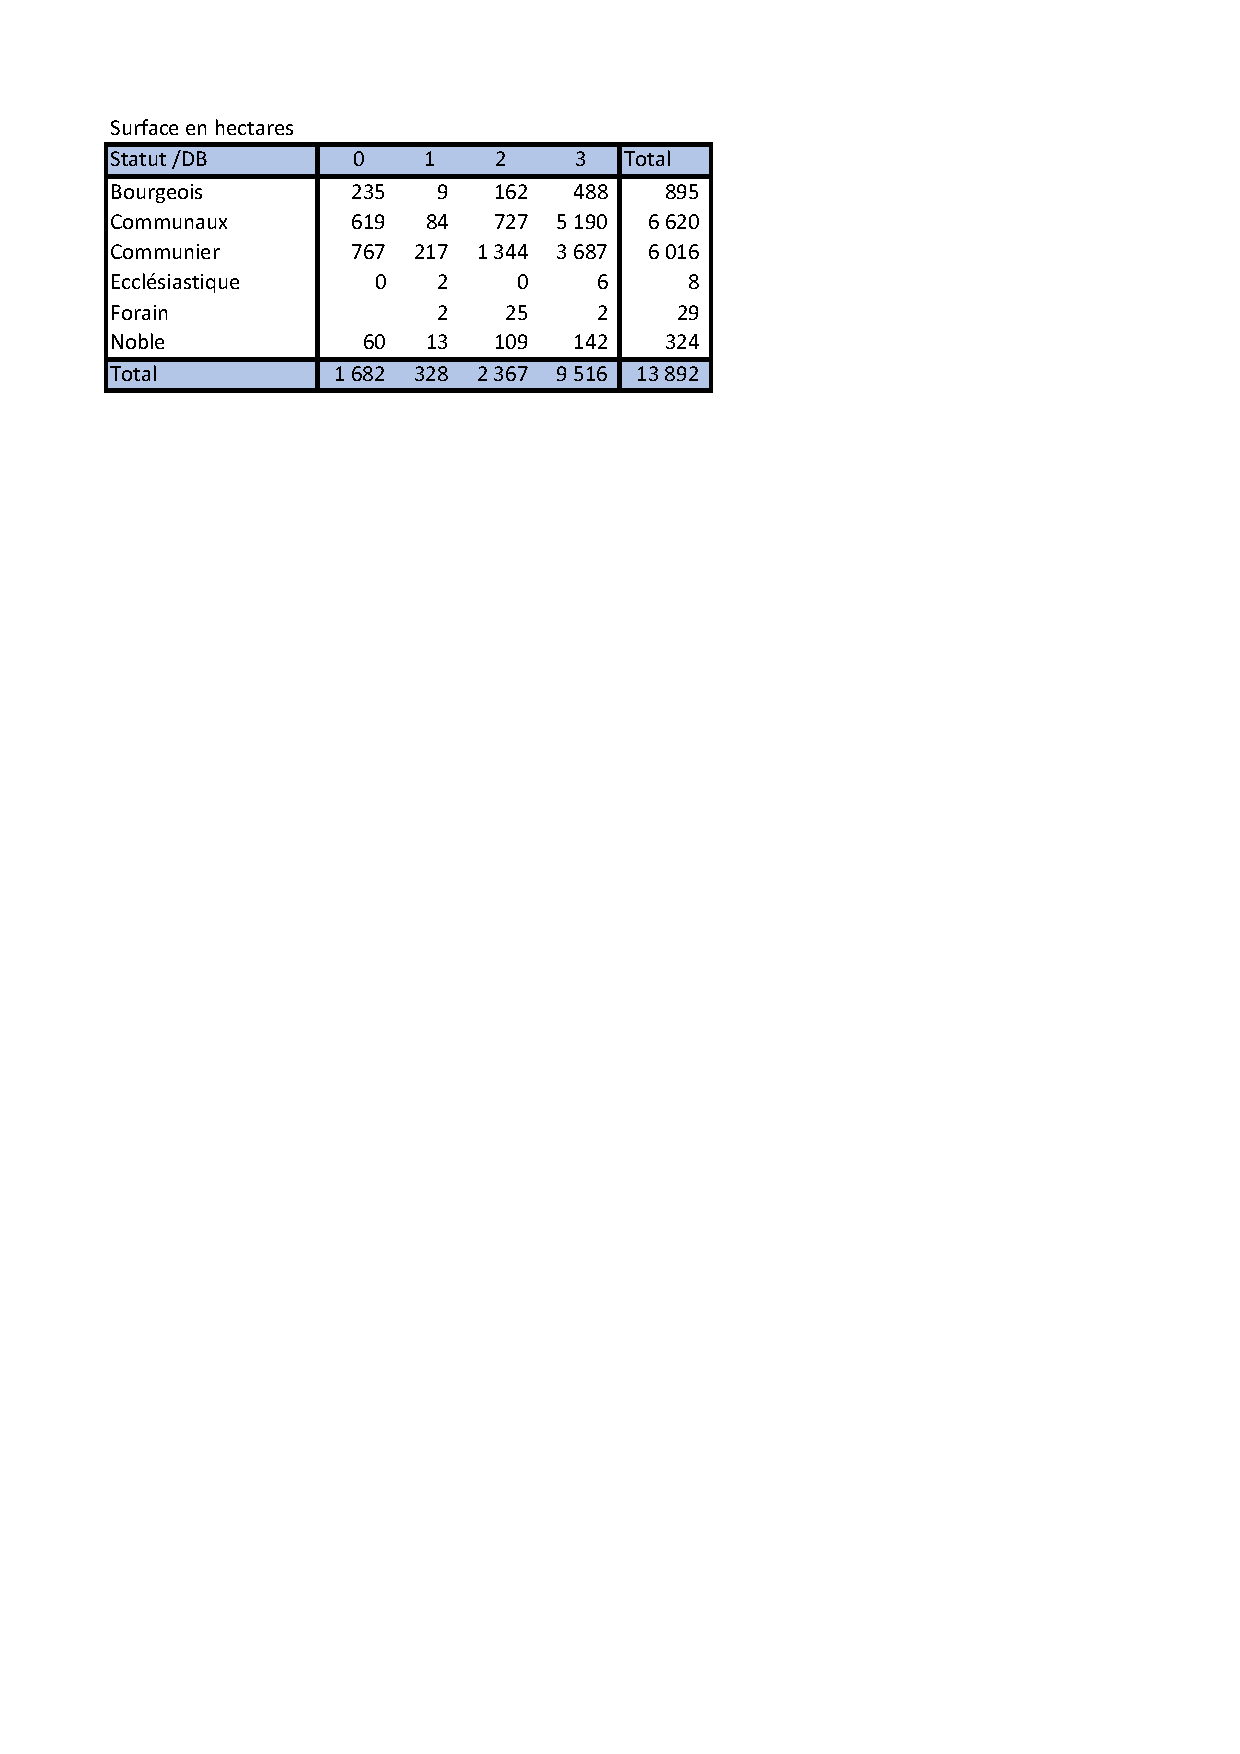
\includegraphics[
		width=\textwidth,
		trim=0cm 23cm 0cm 2cm,
		clip
		]
		{tables/3_SurfStatutDB.pdf}
		\tabcaptionindex{tab:StatutDB}{Superficie par statut et Degré de Bonté}
	\end{table}
	
	
	
	Une très nette majorité de terrains productifs (degrés 1 et 2) pour les particuliers.
	
	
	\begin{table}[htbp]
		\centering
		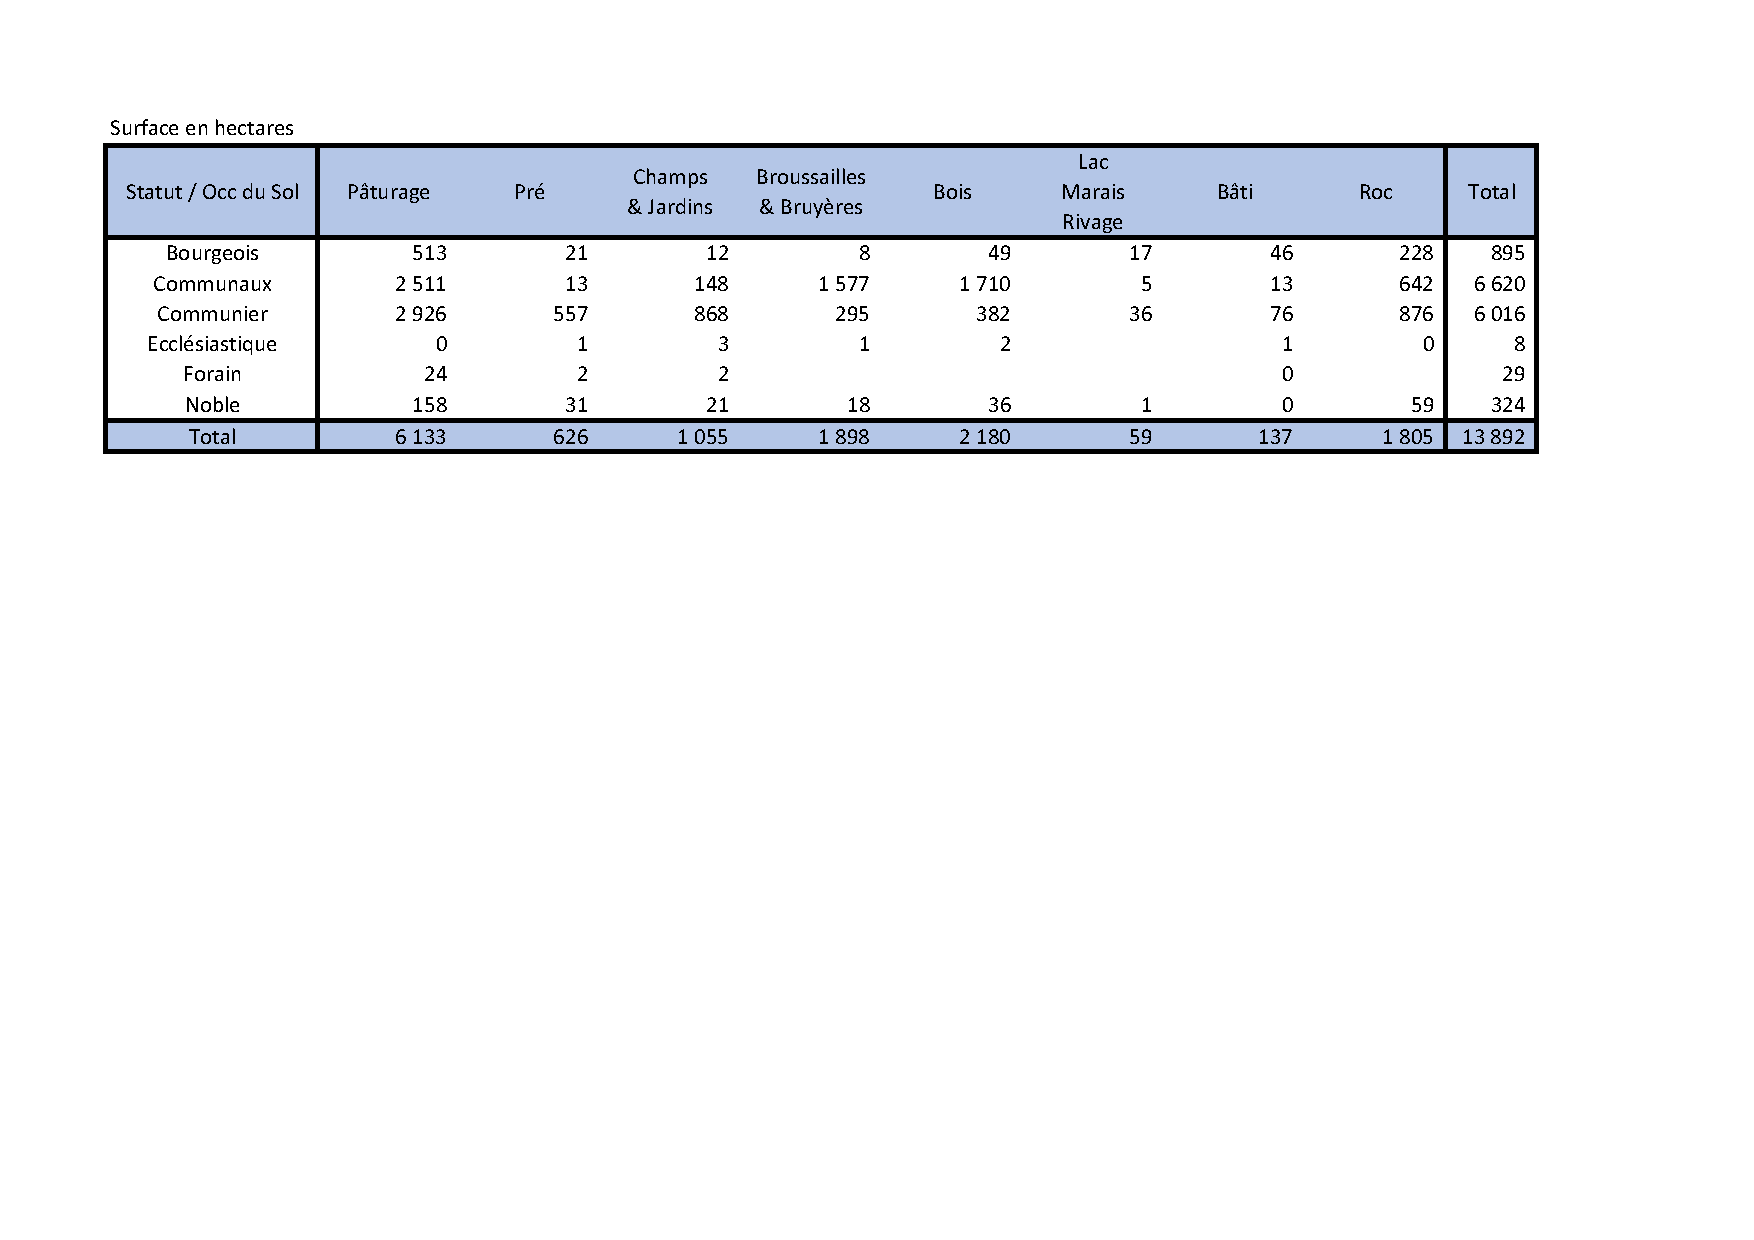
\includegraphics[
		width=\textwidth,
		trim=0cm 13cm 0cm 2cm,
		clip
		]
		{tables/3_SurfStatutOccSol.pdf}
		\tabcaptionindex{tab:Statut_OccSol}{Superficie par statut et Occupation du Sol}
	\end{table}
	
	
	Si au global, les surfaces des communaux et celles possédées par les communiers sont du même ordre de grandeur, il en est différemment lorsque nous regardons le détail par l’utilisation du sol. Ainsi les communaux détiennent \texttt{78\%} des bois et \texttt{58\%} des rocs. Les communiers possèdent \texttt{52\%} des pâturages (et en ajoutant les autres particuliers dont principalement les bourgeois et les nobles, nous atteignons \texttt{63\%} des surfaces en pâturage.
	
	
	
\section{Les propriétaires privés}
	
	Si nous excluons les Communs et les propriétés des institutions ecclésiastiques, nous avons 864 propriétaires privés.
	Dans cette analyse, l'ensemble des propriétaires privés est étudié sans distinction de statut social. Les habitants de Beaufort, les nobles et  les bourgeois  sont ainsi considérés comme une seule population statistique. Ce choix ne revient pas à nier les différences de statut ou de fonction entre ces groupes, mais répond à l'objectif de cette étude, qui est d'analyser la répartition de la propriété privée dans son ensemble. Tous ces acteurs interviennent en effet sur un même marché foncier, acquièrent, héritent ou aliènent des biens selon des mécanismes comparables et participent à la structuration du paysage foncier de la paroisse. Il ne semble pas que ce soit le statut qui fragmente le foncier. La discrimination se fait sans doute davantage sur la profession : les notaires sont des propriétaires importants (Blanc, Cornu, Doix, Chevallier-Joly) et ils ne sont pas forcément "Bourgeois" .
	
	\subsection{Précautions d'interprétation des patrimoines fonciers}
	
	L'analyse de la propriété foncière à partir de la Mappe Sarde ne peut se limiter à une comparaison des surfaces possédées par chaque propriétaire:
	
	En premier lieu, les différentes catégories d'occupation du sol correspondent aussi à des fonctions différentes. Certains bâtiments relèvent d'une logique résidentielle ou immobilière, d'autres sont des outils d'exploitation (granges...) tandis que les prés, les champs, les pâturages, les bois et les broussailles participent, à des degrés divers, au fonctionnement de l'économie agro-pastorale. Les surfaces rocheuses, bien qu'elles soient souvent associées aux espaces d'altitude, constituent  une ressource productive limitée. 
	
	L'altitude doit également être interprétée avec précaution. L'altitude minimale de l'ensemble des biens d'un propriétaire n'est pas toujours représentative de son activité. La possession d'une maison ou de quelques parcelles dans la vallée peut masquer un patrimoine pastoral essentiellement constitué de montagnes d'altitude. 
	Ainsi, par exemple, le cas de Claude Blanc illustre bien cette dissociation. Premier propriétaire de pâturages de la paroisse, il possède également un patrimoine bâti exceptionnel (65 parcelles), principalement situé dans la vallée. La concentration de ces biens immobiliers n'est certainement pas liée à l'exploitation pastorale et témoigne vraisemblablement d'une seconde logique patrimoniale fondée sur l'investissement immobilier.
	Pour étudier les stratégies liées à l'estivage, nous avons trouvé préférable de considérer spécifiquement la distribution en étage des pâturages pris isolément plutôt que celle de l'ensemble des parcelles.
	
	Par ailleurs, la composition d'un patrimoine ne permet pas d'identifier automatiquement le mode d'exploitation du propriétaire. Une faible surface de prés ou de champs ne signifie pas nécessairement l'absence d'une activité pastorale importante. Dans le Beaufortain du XVIIIe siècle, les capacités d'hivernage demeurent limitées par les ressources fourragères et par la taille des bâtiments d'exploitation. Le foin se transporte à dos d'homme ou de mulet. Les grands troupeaux estivant en montagne ne correspondent donc jamais à de grandes exploitations en basse altitude. Les chalets d'hivernage ne peuvent contenir que quelques vaches. Ainsi, les animaux confiés en estivage peuvent appartenir à une multitude de propriétaires différents et retourner hiverner dans leurs exploitations respectives. Et réciproquement, les animaux possédés en propre peuvent être répartis chez une multitude de "clients" pour hivernage. L'étendue des pâturages ne peut donc pas être mise en relation directe avec les seules capacités d'hivernage du propriétaire.
	\\
	
	Le livre de raison de Joseph Blanc illustre parfaitement cette dissociation entre propriété foncière et localisation du cheptel. En 1771, le plus important propriétaire de bétail de la vallée répartit ses animaux dans quarante foyers différents.
	
	\begin{quote}
		« Le livre de raison de Me Joseph Blanc [...] nous donne des indications sur le lieu d'hiverné de ses vaches : en 1771, il a placé cent dix-huit vaches ; quatre à Palud, neuf à Saint-Sigismond, trois à l'Hôpital, une à Villard, trois à Hauteluce et quatre-vingt quatorze à La Pierre (dans quarante foyers). »
		\footcite[58]{HViallet1993}
	\end{quote}
	
	Cette pratique confirme qu'il serait hasardeux de déduire la taille ou le fonctionnement d'une exploitation à partir du seul patrimoine foncier décrit par la Mappe Sarde.
	
	L'analyse proposée dans ce chapitre ne vise donc pas à classer mécaniquement les propriétaires selon des critères quantitatifs, mais à mettre en évidence les principales formes d'organisation des patrimoines que peut nous apporter la Mappe, en croisant plusieurs indicateurs.
	
	
	Remarque : il est fait mention de 229 indivisions et 635 propriétaires individuels: les analyses qui vont suivre n'ont pas pu reconstruire la réalité de chaque propriétaire distinct pour autant qu'il dispose d'un patrimoine en propre et d'une portion en indivision.
	
	
	\subsection{Analyse des propriétaires privés}
	

	Nous avons classé les 864 propriétaires par surface possédée, et nous avons formé 10 groupes de taille identique (décile).
	
	
	\begin{table}[htbp]
		\centering
		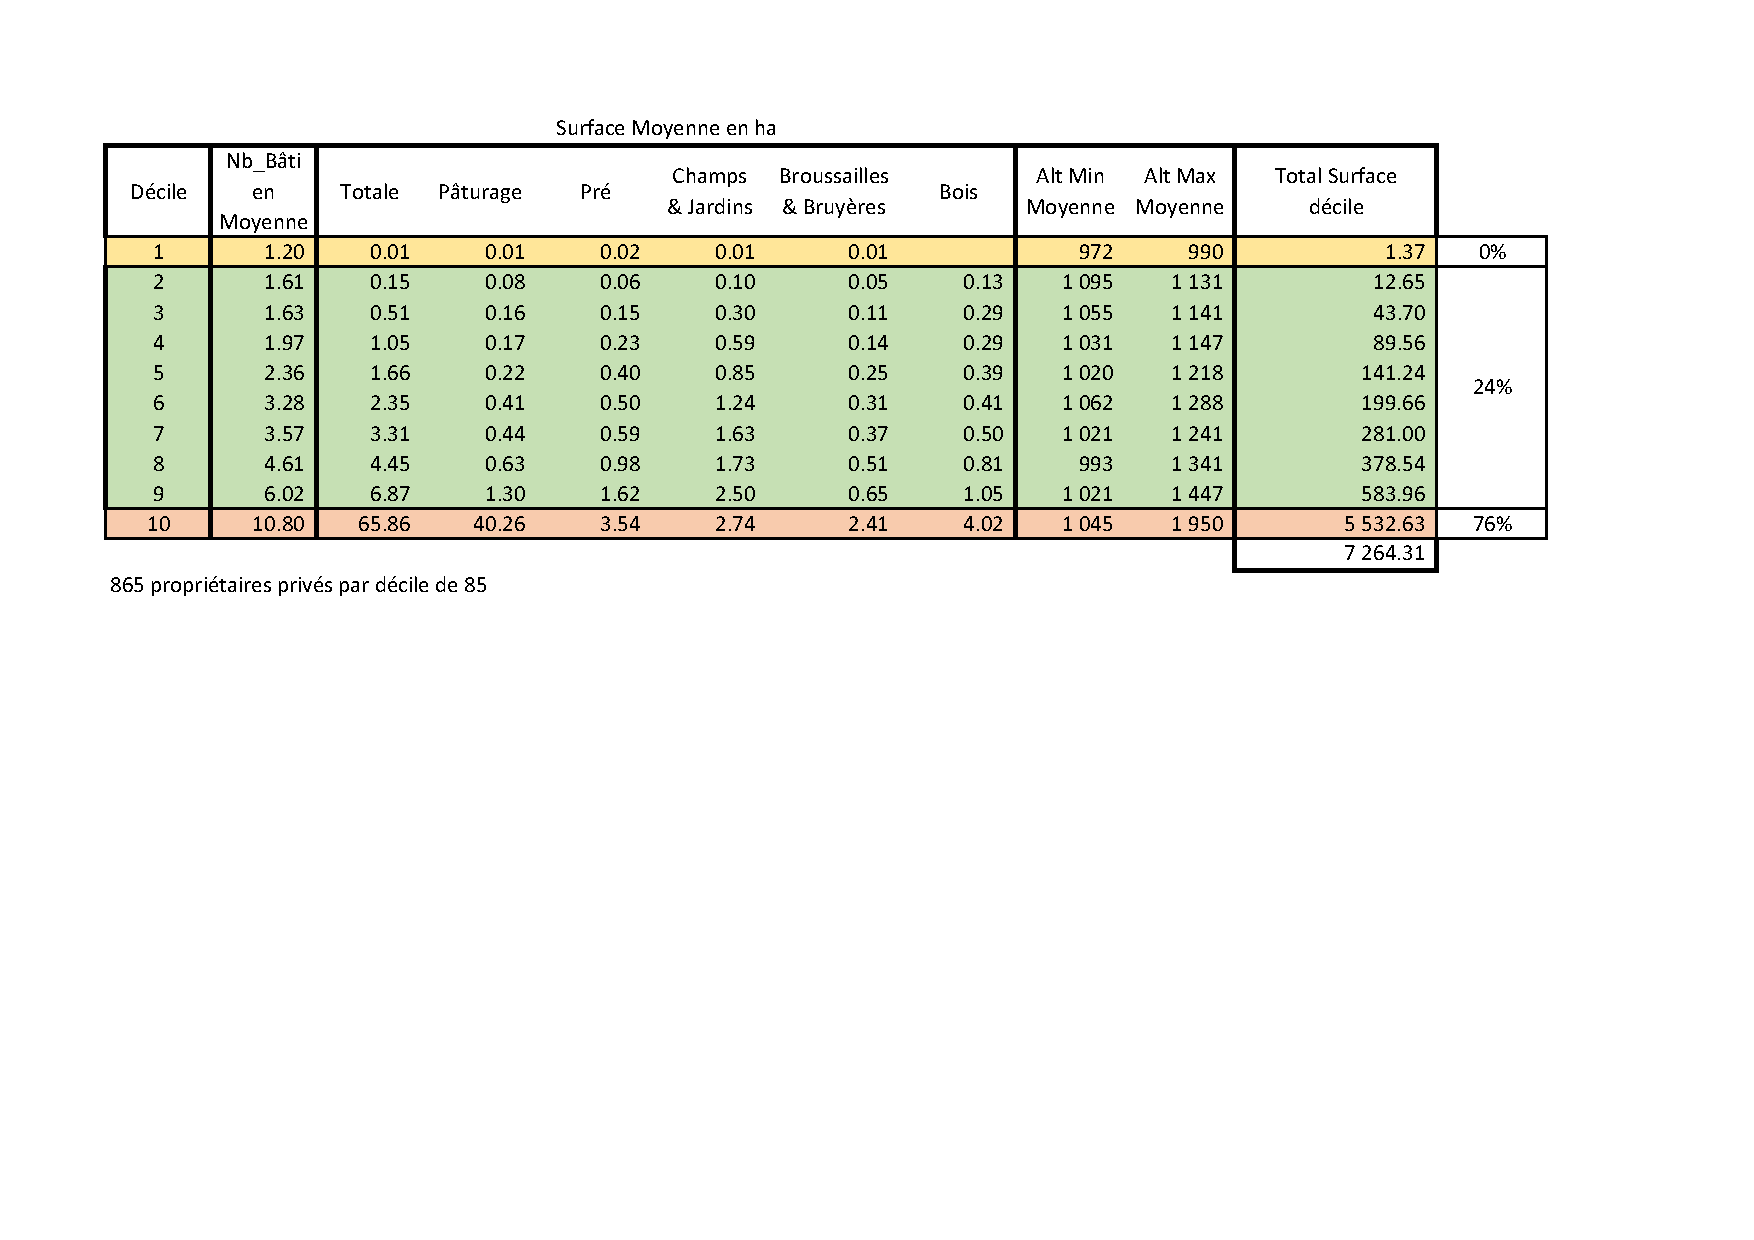
\includegraphics[
		width=\textwidth,
		trim=0cm 10cm 0cm 0cm,
		clip
		]
		{tables/3DecilesProprietairesPrivés.pdf}
		\tabcaptionindex{tab:DecilePP}{Propriété privée par décile}
	\end{table}
	
	
	Remarque : il ne faut pas surinterpréter le premier décile, il n'est pas synonyme de pauvreté : il contient des propriétaires de maisons sans terrain cultivable, il peut s'agir d'artisans ou de commerçants tout à fait prospères. 
	\\
	Le classement des 864 propriétaires privés par déciles de superficie met en évidence une progression régulière des patrimoines jusqu'au neuvième décile, puis une rupture très nette au sommet de la distribution. Les neuf premiers déciles regroupent des patrimoines dont la surface moyenne passe progressivement de 0,01 ha à 6,87 ha. 
	
	
	
	Le dixième décile atteint en revanche 65,86 ha en moyenne, soit près de dix fois plus que le neuvième décile.
	
	Cette rupture ne s'explique pas par une augmentation générale de toutes les catégories de terres. Les champs et jardins progressent jusqu'au neuvième décile, mais plafonnent ensuite : ils passent seulement de 2,50 ha en moyenne dans le neuvième décile à 2,74 ha dans le dixième. Les prés augmentent davantage, de 1,62 ha à 3,54 ha, mais sans commune mesure avec les pâturages, qui passent de 1,30 ha à 40,26 ha. La différence entre les grands propriétaires et le reste de la population ne réside donc pas dans la possession de terres cultivées, mais dans la concentration des pâturages.

\vspace{1em}

	L'altitude confirme cette lecture. L'altitude minimale moyenne varie peu d'un décile à l'autre, autour de 1 000 m. En revanche, l'altitude maximale moyenne augmente nettement dans les derniers déciles, pour atteindre 1 950 m dans le dixième. Les plus grands patrimoines ne se distinguent donc pas par une implantation plus basse dans la vallée, mais par leur extension vers les espaces d'altitude.
	
	Le nombre moyen de parcelles bâties suit également une progression régulière, de 1,2 bâtiment dans le premier décile à 10,8 dans le dernier. Cette croissance du bâti reste toutefois beaucoup moins brutale que celle des pâturages. Elle suggère une plus grande complexité des grands patrimoines, sans suffire à expliquer leur poids foncier.
	
\vspace{1em}
	
	Ainsi, les neuf premiers déciles traduisent surtout une gradation progressive des patrimoines privés. Le dernier décile constitue en revanche une catégorie à part : celle des propriétaires qui concentrent de grands espaces pastoraux. Ces derniers ne représentent qu'un dixième des propriétaires privés, mais détiennent 5.532,63 ha sur un total de 7.264,31 ha, soit environ 76 \% de la surface privée observée. Cette concentration souligne le rôle décisif des pâturages d'altitude dans la hiérarchie foncière du beaufortain.
	
	\subsection{Les propriétaires du dernier décile : entre investisseurs et grandes familles d'exploitants}
	
	L'analyse du dernier décile invite à une certaine prudence dans l'interprétation des patrimoines. La composition des biens (prés, champs, pâturages, bois ou broussailles) ne permet pas, à elle seule, de reconstituer le mode d'exploitation des propriétés. Les pratiques pastorales du Beaufortain au XVIIIe siècle sont trop complexes pour déduire automatiquement, à partir de la seule structure foncière, si un propriétaire exploitait directement ses montagnes, donnait des animaux en remue ou tirait simplement un revenu de ses biens. 
	
	En revanche, certains propriétaires peuvent être identifiés avec davantage de certitude comme des investisseurs fonciers. La qualité de \textit{bourgeois}, de \textit{noble}, de \textit{notaire}, d'\textit{avocat} ou encore de membre du clergé, lorsqu'elle est explicitement mentionnée dans les registres, prouve une activité principale étrangère à l'exploitation agricole. Leur présence parmi les plus grands propriétaires traduit ainsi l'existence d'investissements fonciers réalisés par des élites urbaines ou administratives.
	
	Pour les autres propriétaires du dixième décile,  il paraît préférable de suspendre toute conclusion sur leur mode d'exploitation. Les données cadastrales ne permettent pas de distinguer avec un grand exploitant d'un simple propriétaire foncier.
	
	En revanche, l'apport de la cartographie ouvre un éclairage intéressant. Nous avons affiché sur une carte les noms des  gros propriétaires (ceux du dernier décile) en limitant l'affichage aux parcelles au-dessus de  1\,600~m. 
	
	
	\begin{landscape}
		\thispagestyle{empty}
		
		\begin{figure}[p]
			\centering
			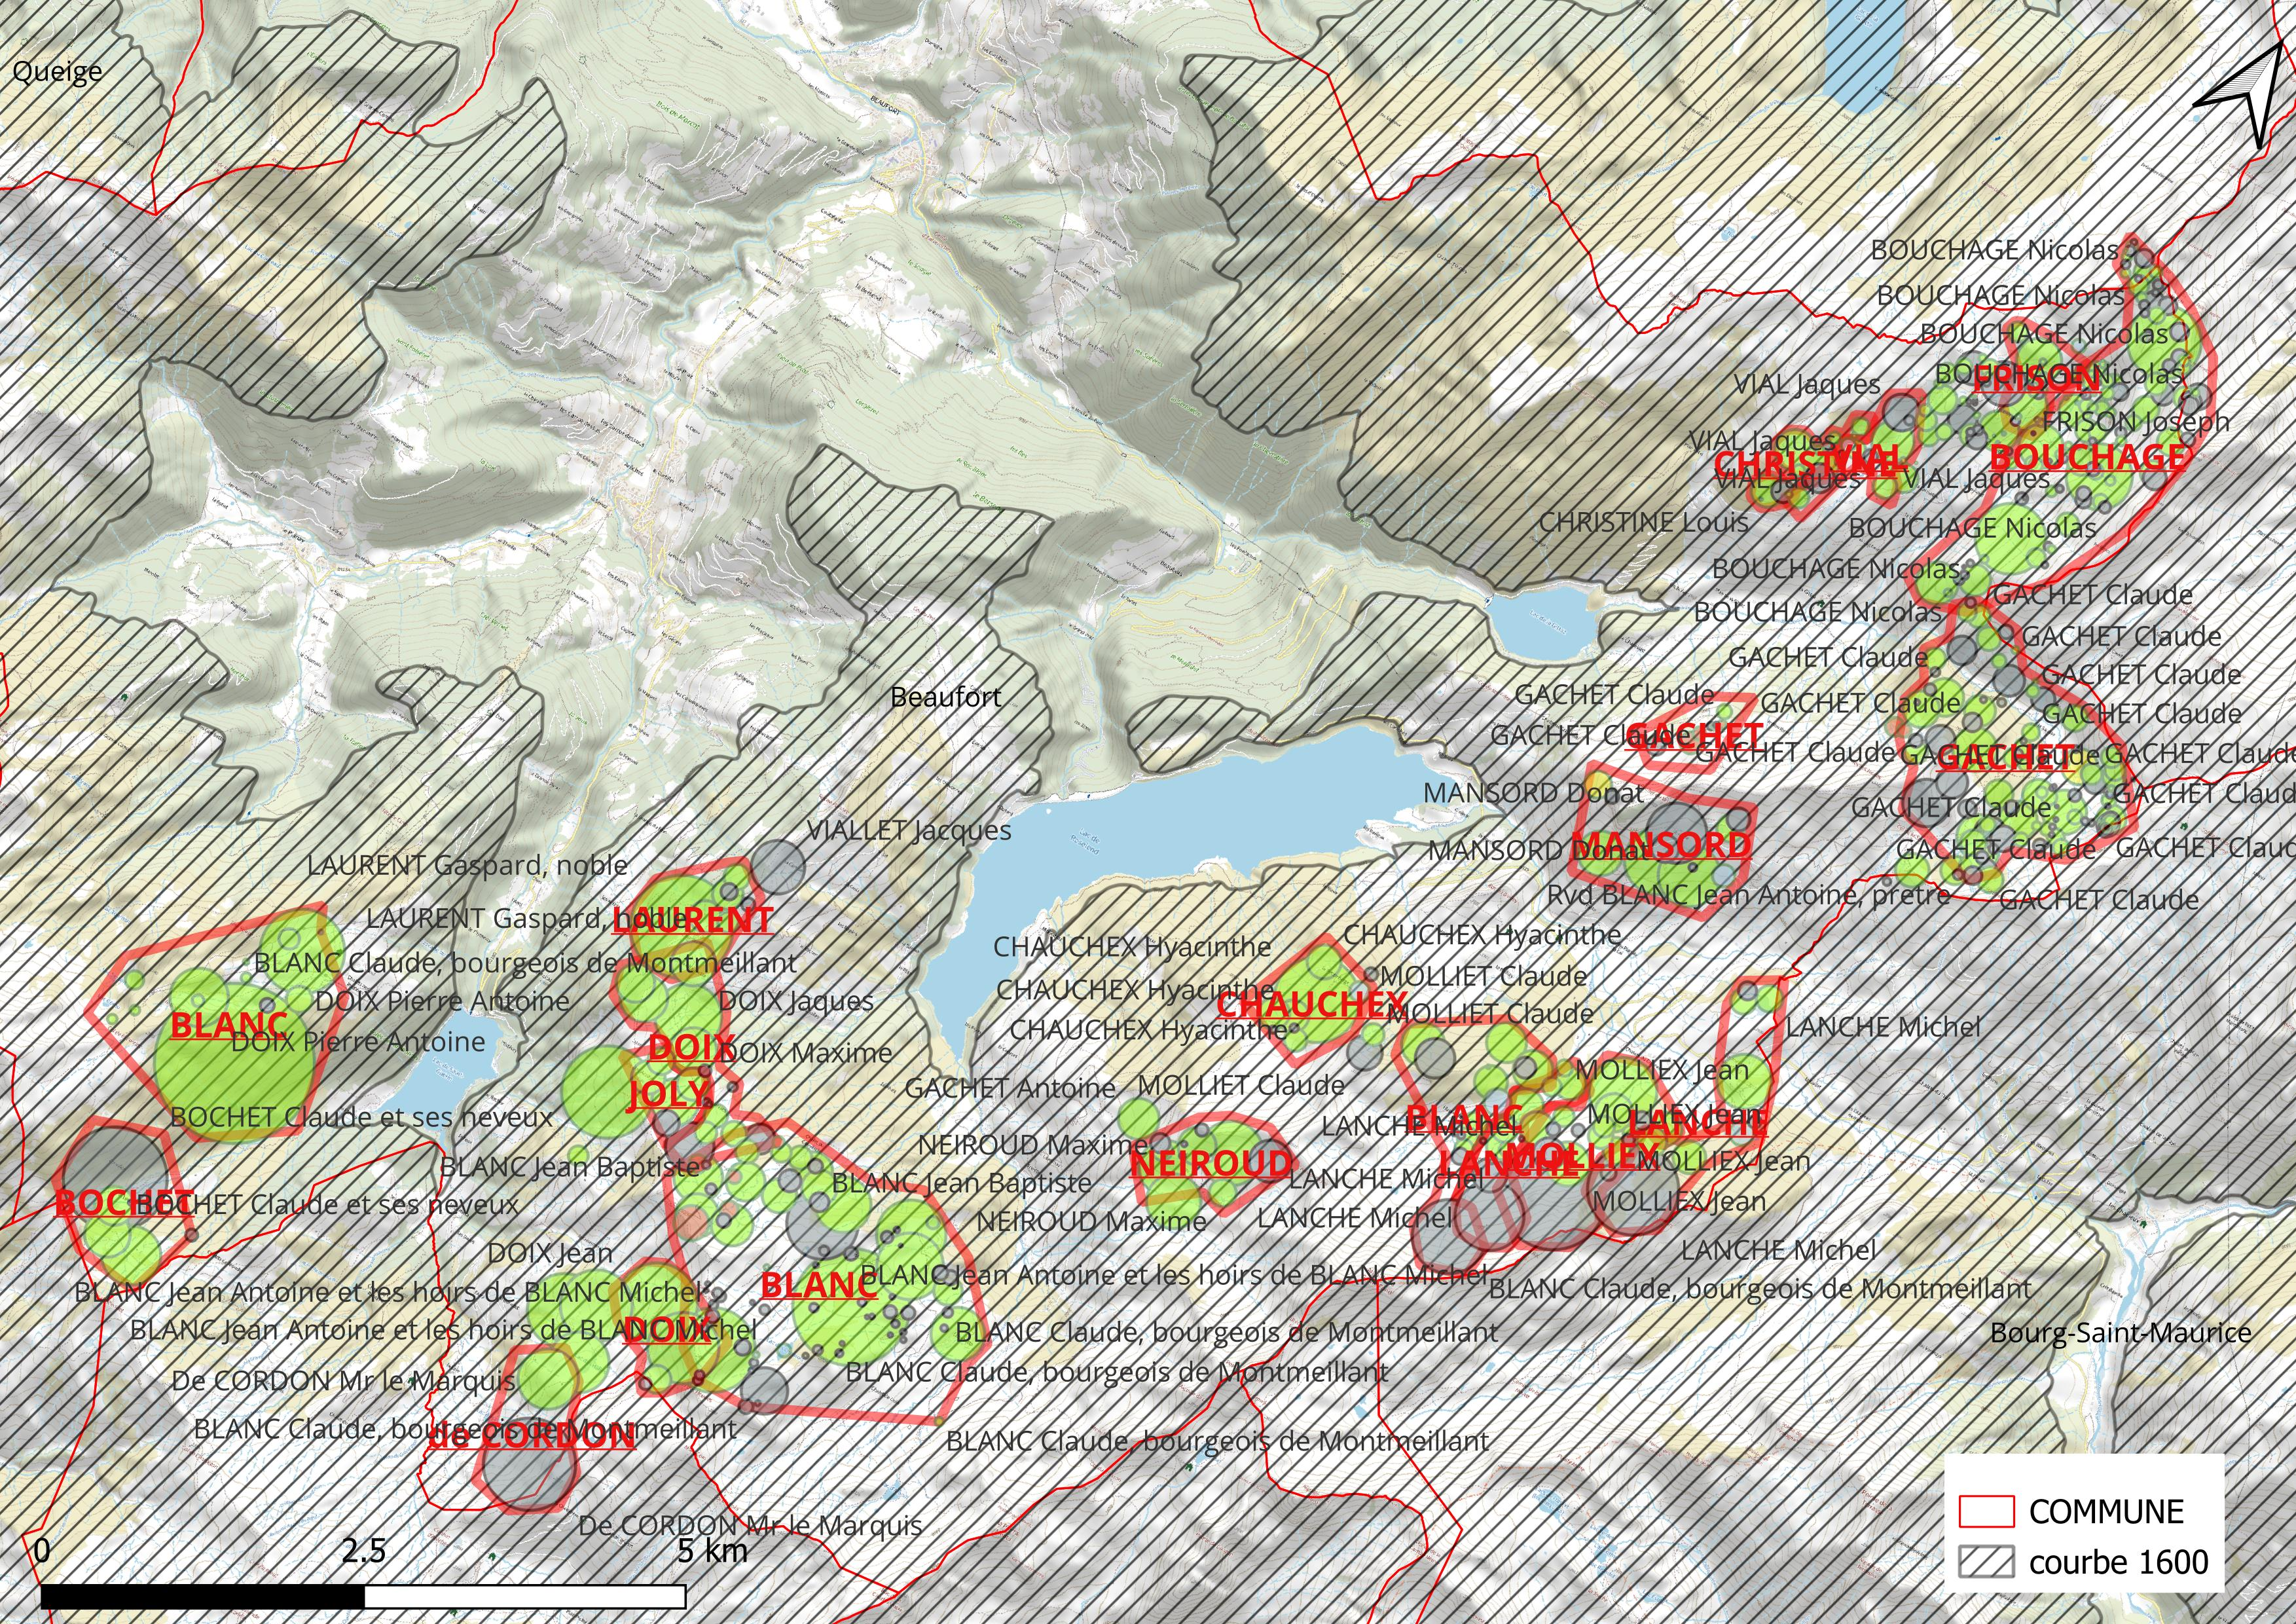
\includegraphics[
			width=\linewidth
			]{figures/3 Carte des grandes familles.jpg}
			\caption{Répartition géographique des patronymes du décile 10}
			\label{GrdesFamilles}
			\idxcarte{Fig.~\thefigure{} -- Répartition géographique des patronymes du décile 10}
		\end{figure}
		
	\end{landscape}
	Il apparaît alors un regroupement évident d'un même patronyme dans des zones où le patronyme est soit majortaire soit même exclusif. Cela fait apparaître plusieurs ensembles fonciers cohérents. Les différentes branches d'une même famille possèdent des parcelles contiguës ou très proches les unes des autres, formant de véritables noyaux patrimoniaux. Une telle organisation ne peut raisonnablement être considérée comme le fruit du hasard. Elle traduit vraisemblablement la permanence de grandes familles implantées de longue date dans les mêmes secteurs de montagne. La dispersion des biens entre plusieurs propriétaires portant le même patronyme s'explique probablement par les partages successoraux successifs, qui ont fragmenté la propriété sans remettre en cause son ancrage géographique. Pour autant, cette fragmentation juridique n'implique pas nécessairement une fragmentation de l'exploitation. Dans une économie pastorale où les alpages nécessitent une organisation collective des travaux, il est plausible que certaines de ces branches familiales aient continué à exploiter leurs montagnes de manière concertée ou complémentaire. La Mappe Sarde ne permet toutefois pas de démontrer ces pratiques. Les regroupements spatiaux observés doivent donc être interprétés comme des indices de continuités familiales et d'une probable solidarité économique, plutôt que comme la preuve d'une exploitation commune. Il suffit par ailleurs qu'un propriétaire dispose seul ou avec sa famille élargie d'un petit alpage  (10 ou 20ha ) mais que celui-ci soit situé stratégiquement à côté d'un grand commun, pour que sa capacité à conduire un très grand troupeau n'ait rien à envier aux très gros propriétaires.
	
	\begin{table}[htbp]
		\centering
		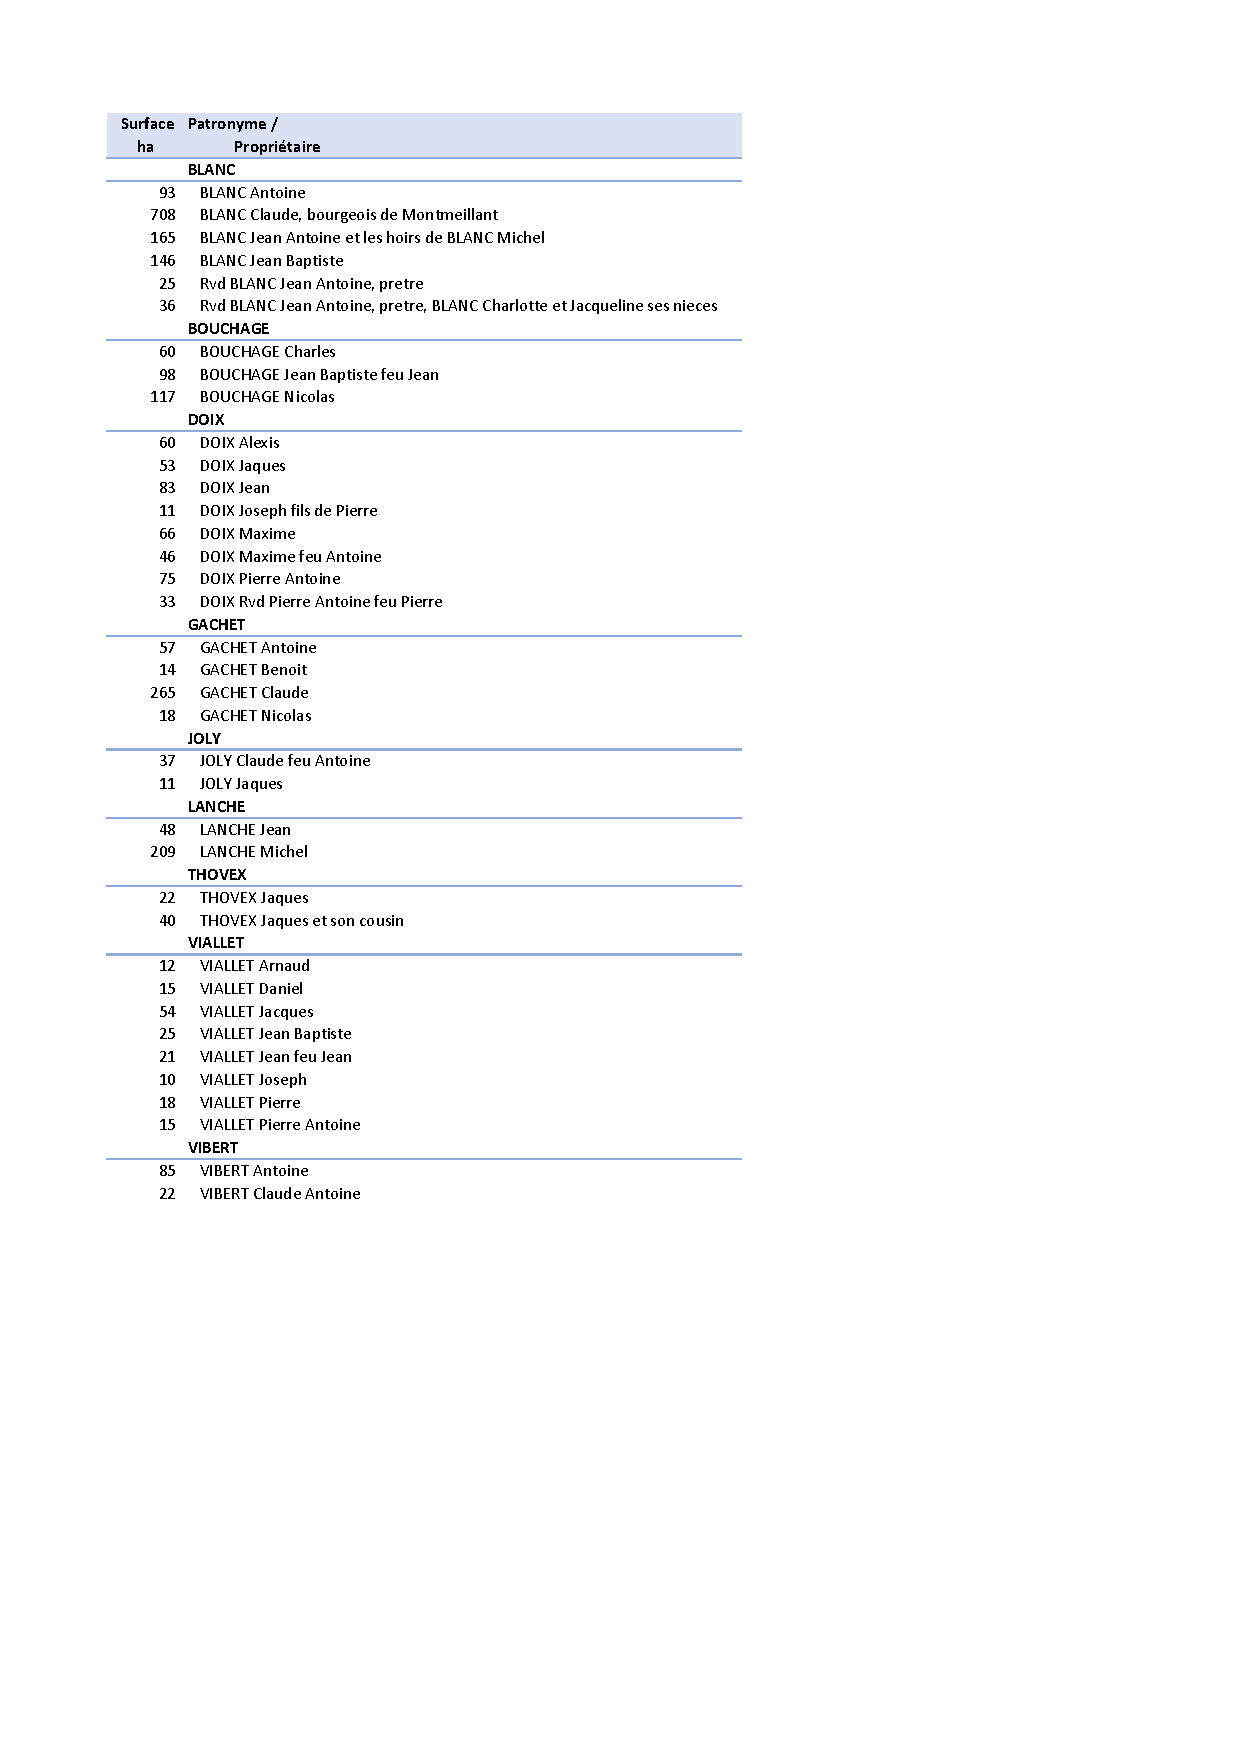
\includegraphics[
		width=\textwidth,
		trim=0cm 8cm 0cm 0cm,
		clip
		]
		{tables/3_PatronymesDecile10.pdf}
		\tabcaptionindex{tab:DecilePatronyme}{Propriétaires du décile10 par patronyme}
	\end{table}
	
	Cette organisation peut être rapprochée des mécanismes décrits par Nicolas Mouthon pour les montagnes à consortage.
	
	\begin{quote}
		« La règle successorale imposant partout le partage des biens entre les fils [...], le Bouchoz [...] est devenue une « petite grande montagne » par la volonté des héritiers de rester dans l'indivision. Ce type d'albergement [...] semble avoir été à l'origine de plusieurs montagnes à consortage, toujours par le jeu des partages d'héritage. »
		\footcite[120]{Mouthon2019MontagnesMedievales}
	\end{quote}
	
	
	\medskip
	Un autre point reste invisible: nous savons que la fabrication de gruyère exige un troupeau important. Nous ne savons pas si tous les propriétaires d'alpages se sont mis à la fabrication du gruyère. L'arrivée de ce nouveau produit de l'élevage a dû se faire progressivement tout au long du XVIIe siècle. Peut-être existe-t-il encore au XVIIIe siècle des petits éleveurs qui sont restés sur une fabrication des fromages traditionnels (vacherin, tomme...).
	
	\medskip
	Ainsi, l'étude du dernier décile ne conduit pas à opposer exploitants et investisseurs. Elle met plutôt en évidence la coexistence de plusieurs formes de grandes propriétés et en parallèle plusieurs formes de grandes exploitations : d'une part des patrimoines détenus par des élites sociales clairement identifiables, d'autre part ceux de familles paysannes dont l'ancienneté et la cohérence spatiale des possessions suggèrent un rôle majeur dans l'exploitation des hautes montagnes.
	
	\medskip
	Afin de dégager d'éventuelles tendances, le décile supérieur des propriétaires, c'est-à-dire les 10\% possédant les plus grandes superficies, a été subdivisé en quatre quartiles de taille égale. Cette méthode ne compare donc pas l'ensemble de la population, mais les différents niveaux de richesse foncière au sein des plus grands patrimoines. 
	
	\vspace{1em}
	
	Le dixième décile regroupe les 84 plus gros propriétaires mais l'éventail est très large, il commence 9,2ha pour plafonner à 707ha.
	
	Si les 21 propriétaires du quartile Q1 sont dans la parfaite continuité de la progression des neuf premiers déciles, on constate que la rupture se fait à partir du quartile Q2. On peut donc considérer 63 propriétaires comme étant véritablement à part des autres propriétaires de la commune
	
\begin{table}[htbp]
	\centering
	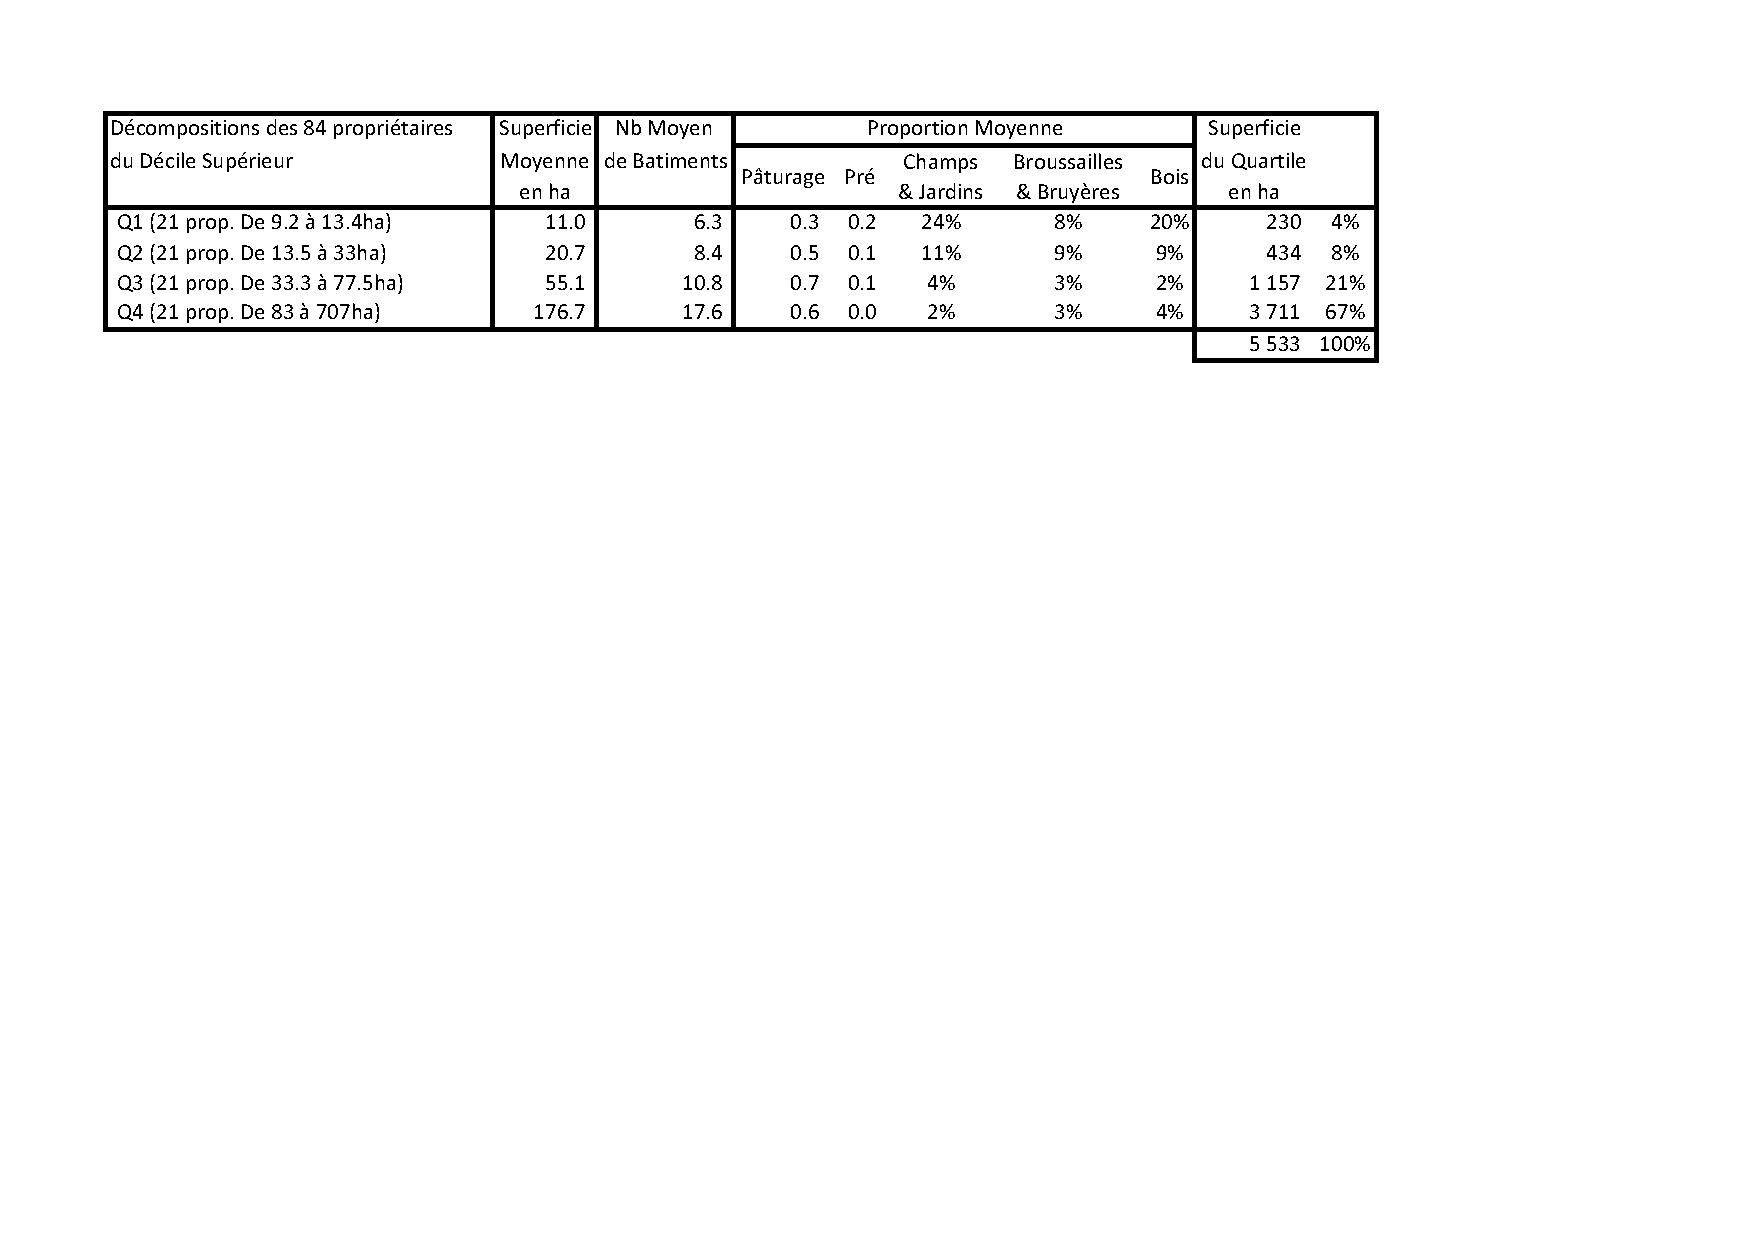
\includegraphics[
	width=\textwidth,
	trim=0cm 14cm 0cm 0cm,
	clip
	]
	{tables/3_QuartileDecile10.pdf}
	\tabcaptionindex{tab:QuartileDecile}{Analyse du Décile Supérieur}
\end{table}
	
	Deux catégories se distinguent:
	
	La première concerne les propriétaires dont le statut social est explicitement connu. Bourgeois, nobles, notaires ou marchands apparaissent comme des investisseurs susceptibles d'acquérir des montagnes non pour les exploiter directement mais pour en tirer un revenu. Les contrats d'ascensement étudiés par Hélène Viallet montrent en effet qu'une montagne constitue au XVIIIe siècle un véritable capital foncier produisant une rente, fréquemment acquittée en gruyères.
	
	\begin{quote}
		« Le mode d'exploitation le plus fréquent pour une grande montagne est donc le fermage, dénommé en Savoie acensement ou admodiation. [...] Le 22 décembre 1755, Joseph Blanc ascense sa montagne de Conchettes à Joseph Chevallier-Joly, sous la censé de 44 quintaux de gruyère à son choix. »
		\footcite[113]{HViallet1993}
	\end{quote}
	
	L'existence de ces contrats montre que la possession d'une montagne n'implique pas nécessairement son exploitation directe. Le propriétaire peut en retirer un revenu sans participer lui-même à la conduite des troupeaux.
	
	\begin{table}[htbp]
		\centering
		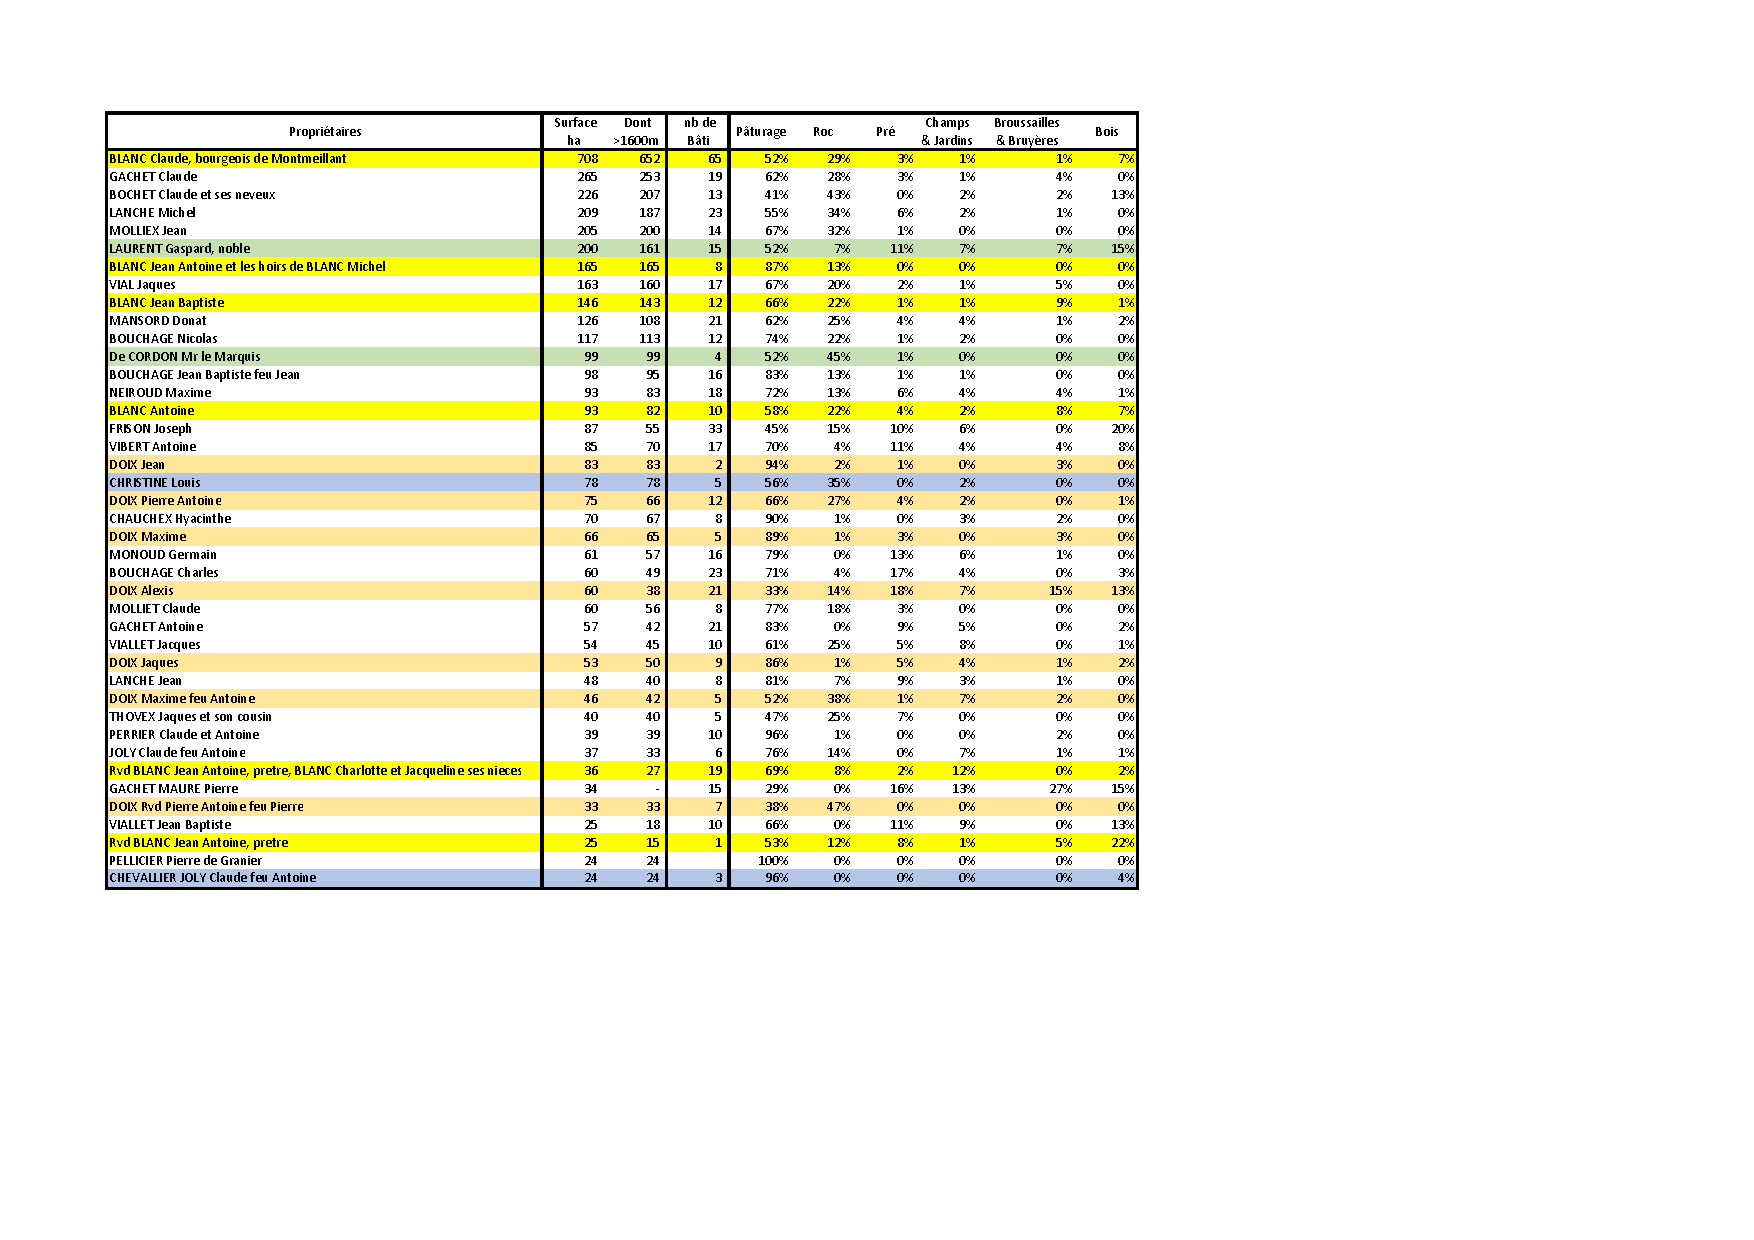
\includegraphics[
		width=1.40\textwidth,
		trim=0cm 5cm 0cm 1.9cm,
		clip
		]
		{tables/3_41PremiersDecile10.pdf}
		\tabcaptionindex{tab:41Premiers}{Liste de 41 plus gros propriétaires}
	\end{table}
	
	Les propriétaires surlignés (17 sur 41) appartiennent à des familles nobles ou des familles qui ont produit des notaires.
	
	Une seconde catégorie concerne les grands communiers du Beaufortain. Les contraintes techniques de l'élevage limitent alors fortement les capacités d'hivernage : les étables restent de dimensions modestes, les réserves de foin doivent être récoltées et transportées manuellement, et chaque exploitation ne peut généralement conserver qu'un nombre restreint de vaches durant l'hiver. La maîtrise d'une montagne privée pourrait ainsi correspondre moins à la possession d'un très grand troupeau personnel qu'à la capacité d'accueillir en estivage les animaux appartenant à de nombreux petits propriétaires.
	
	Dans ce système, le patrimoine foncier ne reflète donc pas directement la taille du troupeau possédé. Les pratiques de pension, de remue, les multiples formes de faire-valoir ou encore les copropriétés de bétail rendent impossible toute reconstitution des exploitations à partir de la seule structure cadastrale.

Cette concentration foncière observée dans la Mappe Sarde est d'ailleurs cohérente avec les critiques formulées dès le XVIe siècle à l'encontre de l'accaparement des pâturages par les plus riches habitants du Beaufortain.

\begin{quote}
	« Cette tendance, qui mène à la constitution des montagnes particulières ou privées [...]. En 1552, une supplique des habitants du mandement de Beaufort explique de façon très claire que les plus riches d'entre eux accaparent les pâturages communs aux dépens des plus pauvres : "icelles communautés se gaudissent et jouyssent par gens du pays riches ayant puissance de bestail de sorte que le povre menu peuple d'icelles est quasiment frustré". »
	\footcite[125]{Mouthon2019MontagnesMedievales}
\end{quote}

Sans permettre d'établir une continuité directe entre cette plainte et la situation cadastrale de 1732, la forte concentration des montagnes privées observée dans la Mappe apparaît néanmoins cohérente avec un phénomène de longue durée déjà signalé par les contemporains.
	
	
	
	
	

\chapter{Le Beaufortain entre société d'Ancien Régime et modernité}

\section{L'émergence d'un capitalisme rural : l'exemple de la famille Blanc}
	\subsection{La constitution d'un patrimoine alpagiste avant la Mappe Sarde}
	
	L'étude des archives privées de la famille Blanc, analysées par Hélène Viallet \footcite{Viallet1990Blanc}, permet de retracer sur plusieurs générations un processus de concentration foncière particulièrement précoce . Dès le premier tiers du XVII\ieme\ siècle, certains propriétaires aisés entreprennent de regrouper des portions d'alpages jusque-là morcelées entre de nombreux détenteurs. Cette évolution accompagne la diffusion de nouvelles techniques de fabrication fromagère et le développement du commerce du gruyère, qui exigent des unités pastorales plus vastes et mieux structurées.
	
	La famille Blanc apparaît comme l'un des principaux acteurs de cette transformation. Claude Blanc, mort vers 1650, figure déjà parmi les plus importants propriétaires fonciers de Saint-Maxime. Selon Viallet, il possède plus de 240 hectares de terres, prés et pâturages répartis entre Arêches, Roselend et la vallée de Saint-Guérin. Il fait partie des premiers notables beaufortains à expérimenter les nouvelles formes d'exploitation liées à la production du gruyère et cherche à accroître la rentabilité de ses montagnes par le regroupement des pâturages.
	
	Son fils Gaspard Blanc poursuit cette politique dans la vallée de Treicol. Entre le milieu du XVII\ieme\ siècle et le début du XVIII\ieme\ siècle, de nombreuses acquisitions sont réalisées auprès de propriétaires originaires d'Aime, de Granier ou des communautés voisines. Les transactions portent souvent sur des fractions indivises de montagnes, révélant l'extrême morcellement hérité des générations précédentes. Cette politique patiente d'achats successifs vise moins l'accumulation de terres dispersées que la constitution d'ensembles cohérents susceptibles d'accueillir des troupeaux importants.
	
	L'exemple de la montagne des Meudes dans la vallée de Treicol illustre particulièrement bien cette dynamique. Entre 1642 et 1714, douze acquisitions successives permettent de constituer un vaste ensemble d'environ 200 hectares pouvant accueillir une centaine de vaches laitières. La documentation conservée qualifie ce processus de « procession », terme qui désigne ici la succession méthodique des achats et échanges nécessaires à la constitution d'un grand domaine alpin. Dans le même temps, la famille Blanc étend son influence sur les secteurs voisins de Conchettes, Dunand et Lavachet, renforçant progressivement sa maîtrise foncière sur l'ensemble de la vallée de Treicol.
	
	Au début du XVIII\ieme\ siècle, cette politique d'acquisition se poursuit encore. Le révérend Jean-Antoine Blanc et son frère Michel interviennent dans les transactions concernant la montagne du Couvercle, tandis que Joseph Blanc complète vers 1750 la constitution de cet ensemble foncier par l'achat des montagnes des Bettières, de Parozan et des Halles. Quelques années auparavant, l'acquisition de l'alpage de Rognoux auprès de son frère Jean-Pierre lui avait déjà permis d'étendre son influence dans la vallée de Saint-Guérin.
	
	Ainsi, bien avant la réalisation de la Mappe Sarde, une partie des grands domaines pastoraux du Beaufortain résulte d'un long processus de concentration foncière engagé dès le XVII\ieme\ siècle. Les acquisitions réalisées par la famille Blanc témoignent de la capacité de certains notables ruraux à mobiliser des capitaux importants afin de constituer de véritables entreprises pastorales. Elles illustrent également le passage progressif d'un système fondé sur le morcellement et les indivisions à une exploitation plus intensive des alpages, adaptée aux exigences croissantes de la production fromagère et du commerce régional.
	
\subsection{Mariage Jospeh Blanc et Charlotte Blanc}	

La concentration foncière opérée par la famille Blanc au cours des XVII\ieme\ et XVIII\ieme\ siècles trouve un écho direct dans la documentation cadastrale de la Mappe Sarde. La carte des parcelles appartenant à la famille met en évidence l'importance du patrimoine contrôlé par les héritiers de cette lignée au moment de la mensuration.

\cartefigure[0.9\textwidth]
{figures/4 Carte Matignon Globale.jpg}
{fig:CarteMatignon}
{Carte des propriétés du Rd Blanc et de ses nièces }

Parmi les principaux détenteurs figurent notamment le révérend Jean-Antoine Blanc ainsi que ses nièces. Cette situation reflète les mécanismes de transmission patrimoniale propres aux familles de notables ruraux. L'une de ces héritières, Charlotte Blanc, épouse en 1732 son cousin Joseph Blanc, futur notaire-insinuateur et secrétaire de la communauté de Saint-Maxime. Cette union contribue à maintenir au sein d'un même groupe familial une partie importante des biens accumulés par les générations précédentes.

La carte met ainsi en évidence que les acquisitions réalisées depuis le milieu du XVII\ieme\ siècle ne se traduisent pas seulement par l'existence de grands domaines pastoraux, mais également par la constitution d'un patrimoine familial dense, réparti dans plusieurs secteurs de la paroisse. La concentration foncière observée dans la Mappe Sarde apparaît dès lors comme l'aboutissement d'une stratégie de long terme associant achats successifs, héritages et alliances matrimoniales.

L'exemple des Blanc illustre ainsi la manière dont certaines familles de notables ont pu consolider leur position économique dans le Beaufortain en articulant étroitement maîtrise foncière, fonctions administratives et réseaux de parenté.

	
	\cartefigure[0.8\textwidth]
	{figures/4 extrait 1a.jpg}
	{fig:ParcellesJABlanc}
	{Extrait des parcelles du Rdv Jean-Antoine BLANC}
	
	\cartefigure[0.3\textwidth]
	{figures/4 extrait 2.jpg}
	{fig:ParcelleFBlanc}
	{Extrait des parcelles de Françoise CHRISTINÉ veuve de Michel BLANC}
	
	\cartefigure[0.3\textwidth]
	{figures/4 extrait 3.jpg}
	{fig:ParcellesChapelleBlanc}
	{Extrait des parcelles qui ont été rayées attribuées à la Mappe des Chapelles }
		

	

	
	\subsection{La descendance de Joseph Blanc et la consolidation du patrimoine familial}
	
	Le mariage de Joseph Blanc avec sa cousine Charlotte Blanc en 1732 marque moins l'aboutissement que le commencement d'une nouvelle phase dans l'histoire patrimoniale de la famille. Héritier d'un important ensemble foncier constitué au cours des générations précédentes, Joseph Blanc poursuit la politique d'expansion familiale en combinant acquisitions privées, contrôle des institutions communautaires et gestion active des alpages.
	
		\cartefigure[0.3\textwidth]
	{figures/4 Genealogie_Blanc.jpg}
	{fig:GenealogieBlanc}
	{Arbre généalogique de la famille Blanc (XVIIe--XIXe siècles)}
	
	Dans la seconde moitié du XVIII\ieme\ siècle, il complète notamment les possessions familiales dans la vallée de Treicol par l'acquisition des montagnes des Bettières, de Parozan et des Halles, tandis que l'achat de Rognoux lui assure une implantation durable dans la vallée de Saint-Guérin. Les revenus tirés de la location de ces alpages et du commerce du gruyère renforcent encore la position économique de la famille.
	
	Cette dynamique ne s'interrompt pas avec sa disparition. Son fils Michel Blanc puis son petit-fils Ambroise Blanc héritent d'un patrimoine considérable qui leur permet de demeurer parmi les principaux notables du Beaufortain. Les générations suivantes continuent à intervenir sur le marché foncier local, profitant notamment des ventes judiciaires et des adjudications publiques qui se multiplient au cours de la période révolutionnaire et du XIX\ieme\ siècle. Ces ventes aux enchères offrent aux familles disposant de capitaux importants l'occasion de renforcer encore leurs positions foncières en rachetant des biens mis sur le marché à la suite de successions difficiles, d'endettements ou de procédures judiciaires.
	L'affranchissement de 1770 et les ventes de communaux qui l'accompagnent constituent une nouvelle étape dans la consolidation du patrimoine familial. Déjà solidement implantés parmi les principaux propriétaires de la paroisse, les Blanc figurent parmi les principaux bénéficiaires des aliénations foncières décidées par la communauté.
	
	Selon Hélène Viallet, Joseph Blanc est le premier acquéreur de ces ventes avec 99 hectares, soit 14,3\,\% de la superficie totale mise sur le marché. Les parcelles qu'il obtient se situent notamment à Roselend, Rognoux, à la Grande Parre ainsi que dans les pâturages des Côtes d'Ani et de l'Arpette. Son neveu Jean-Baptiste Blanc occupe le second rang avec 75 hectares acquis lors de la même opération. À eux deux, ils concentrent ainsi une part importante des terres aliénées par la communauté.\footcite[p.~266-267]{Viallet1990Blanc}
	
	Ces achats ne constituent pas une rupture mais prolongent une politique foncière engagée depuis le XVII\ieme\ siècle. Après avoir constitué de vastes ensembles pastoraux par achats successifs dans la vallée de Treicol et à Saint-Guérin, la famille Blanc profite de la mise sur le marché d'une partie des communaux pour renforcer encore sa position. Les aliénations de la décennie 1770 apparaissent ainsi comme l'un des derniers épisodes d'un long processus de concentration foncière amorcé plus d'un siècle auparavant.
	
	Au-delà des seules acquisitions foncières, cette continuité patrimoniale s'accompagne d'une permanence des fonctions sociales et administratives. Les Blanc demeurent présents dans les professions juridiques et administratives qui avaient assuré leur ascension dès le XVII\ieme\ siècle. Cette double accumulation, foncière et institutionnelle, contribue à faire de la famille l'une des principales lignées de notables du Beaufortain.
	
	L'aboutissement de cette trajectoire est incarné au XIX\ieme\ siècle par la figure du sénateur Blanc. Son accession aux plus hautes responsabilités politiques régionales témoigne de la réussite d'un processus engagé plus de deux siècles auparavant. La puissance sociale de la famille ne repose alors plus seulement sur la possession d'alpages ou de terres agricoles, mais sur un capital économique, relationnel et politique construit progressivement par plusieurs générations. Ainsi, des premières acquisitions réalisées dans la vallée de Treicol au XVII\ieme\ siècle jusqu'à l'émergence d'une figure sénatoriale au XIX\ieme\ siècle, l'histoire des Blanc illustre la capacité de certaines familles montagnardes à transformer une réussite foncière locale en véritable notabilité régionale.
	
	\subsection{Capitalisme rural}
	
	L'exemple de la famille Blanc dépasse donc le cadre d'une  accumulation patrimoniale. Nous assistons à la mise en place progressive d'une véritable entreprise pastorale fondée sur la mobilisation du capital, l'organisation de la production et l'intégration aux circuits commerciaux régionaux.
	
	Le premier élément est l'investissement foncier. Sur plusieurs générations, les Blanc consacrent des capitaux importants à l'acquisition et au regroupement d'alpages auparavant morcelés. Cette politique vise moins la possession symbolique de terres que la constitution d'unités d'exploitation cohérentes capables d'accueillir des troupeaux nombreux et de soutenir une production fromagère importante.
	
	Le second élément réside dans l'organisation même de la production. Chalets, bâtiments d'exploitation, remues et pâturages sont organisés afin d'optimiser la fabrication du gruyère. Les Blanc font venir des fromagers de suisse et l'impose au locataire de leur montagne, ils imposent aussi le règlement  du cens en nature et se réservent l'exclusivité pour l'achat de la totalité de la "fruitière"\footcite[262]{Viallet1990Blanc}. Ils ont propriétaires d'importants troupeaux et gère leur hivernage auprès de nombreux "clients" dans la vallée.
	
	« M. Joseph Blanc possède le troupeau le plus important de la vallée. En 1771, il note dans son livre de raison la mise en hiverne de ses 122 vaches : 9 à Saint-Sigismond, 3 à l'Hôpital, 4 à Pallud, 1 à Villard, 3 à Hauteluce et 94 à la Pierre. Dans une quarantaine de foyers de ce hameau, les deux ou trois vaches du secrétaire apportent une précieuse ressource pendant l'hiver : le preneur garde le lait et le veau. Si la vache ne donne pas de veau, le propriétaire devra payer une pension pour elle, comme pour une génisse. À la belle saison, ces vaches seront louées au montagnard. »
	\footcite[265]{Viallet1990Blanc}
	Le troisième élément est la maîtrise des circuits commerciaux.  Les partenariats noués avec des marchands de Maurienne permettent d'écouler les productions au-delà du marché local, notamment vers le Piémont en mutualisant leurs moyens et se partageant les bénéfices. 
	
	La trajectoire des Blanc est à comparer avec celle observée dans la Gruyère Suisse, où le développement de l'économie fromagère s'accompagne, dès l'époque moderne, d'importants investissements fonciers par les notables de Fribourg: \begin{quote}
		« Au cours du XVII\ieme\ siècle, la situation change considérablement. Grâce à l'intensification des échanges avec les villes du plateau suisse et avec les pays étrangers, des débouchés nouveaux s'ouvrent au commerce de fromages. Le prix du fromage, produit d'exportation de l'économie alpestre étant monté, les prix d'amodiation des pâturages sont également en hausse. Le placement d'argent dans la propriété immobilière alpestre devient une opération financière intéressante pour des personnes possédant des capitaux. »
		\footcite[44]{RuffieuxBodmer1972HistoireGruyere}
	\end{quote}
	 L'inflation et les ressources en fromages utilisées par les armées durant la guerre de Trente Ans: 
	 \begin{quote}
	 	« Ce n'est que pendant la guerre de Trente Ans, lors de la forte hausse du prix des denrées alimentaires en Suisse et à l'étranger, à partir de 1620, que le fromage devient un article d'exportation très recherché. C'est à ce moment que l'État commence également à s'intéresser au commerce de fromages. Par le mandat du 2 septembre 1621, le gouvernement fribourgeois institua une "traitte foraine" de 5 batz à prélever pour chaque quintal de fromage exporté en pays étranger.»
	 	\footcite[60]{RuffieuxBodmer1972HistoireGruyere}
	 \end{quote} 
	Il y a cependant une différence notable, les autorités du canton de Fribourg soutiennent et défendent activement l'activité économique fortement exportatrice, alors que nous ne trouvons aucune trace d'un intérêt particulier des autorités piémontaises pour la production et le commerce de fromage savoyard. 
	Ainsi, en 1665, le gouvernement de Fribourg intervient pour réguler les prix:
	 \begin{quote}
	 	«Attribuant la stagnation dans l'écoulement des fromages et les prix bas réalisés à Lyon à la concurrence acharnée et aux « désordres » des marchands-sujets, LL. EE. craignaient que cet état de choses ne compromît sérieusement l'économie alpestre à laquelle une bonne partie du patriciat fribourgeois était intéressée. Afin de sauvegarder leurs propres intérêts en même temps que l'intérêt de l'État, LL. EE. se décidèrent de faire de ce commerce un monopole et de le confier à une association formée de patriciens.»
	 	\footcite[159]{RuffieuxBodmer1972HistoireGruyere}
	 \end{quote}
	 
	 Si le contexte institutionnel savoyard diffère sensiblement de celui de la Suisse voisine, la comparaison souligne néanmoins l'existence, de part et d'autre des Alpes, de cette forme de capitalisme rural .
	
	Une piste de recherche mérite enfin d'être évoquée. Les trajectoires observées dans le Beaufortain invitent à s'interroger sur les liens entre le développement des productions fromagères savoyardes et l'essor plus ancien des régions suisses productrices de gruyère. Dès le XVII\ieme\ siècle, l'ouverture de débouchés internationaux favorise en Suisse l'investissement de capitaux dans les alpages, la concentration de la propriété pastorale et l'intervention des autorités publiques dans l'organisation du commerce.\footcite[44, 60, 159]{RuffieuxBodmer1972HistoireGruyere}
	
	Dans ce contexte, on peut se demander si le développement des grandes exploitations pastorales du Beaufortain au XVIII\ieme\ siècle ne répond pas également, au moins en partie, à la volonté de s'affranchir de la dépendance commerciale à l'égard des producteurs et des intermédiaires suisses. Les sources actuellement réunies ne permettent pas de démontrer une telle relation. L'étude comparative des politiques commerciales et douanières, des réseaux marchands et des flux fromagers entre la Suisse, la France, la Savoie et le Piémont constituerait à cet égard une perspective de recherche particulièrement intéressante.
	
\section{Litiges de Treicol avec la communauté des Chapelles }	
\label{sec:LesChappelles}
	
	
	
	\subsection{Les limites de la paroisse et le cas particulier de la vallée de Treicol}
	
	L'examen du patrimoine foncier de la famille Blanc fait apparaître une particularité cartographique qui dépasse le seul cadre de l'histoire familiale. Sur plusieurs parcelles appartenant au révérend Jean-Antoine Blanc et à ses nièces, les indications portées sur la Mappe Sarde montrent en effet des radiations destinées à transférer temporairement ces biens dans la mappe de la paroisse voisine des Chapelles.
	
	Au-delà des quelques parcelles listées sur la "Mappe Blanc" nous avons identifié 137 parcelles rayées des registres de la Mappe de Saint-Maxime et transférées sur celle de la paroisse des Chapelles
	
	\cartefigure[0.9\textwidth]
	{figures/4 Carte des Parcelles Transférées aux Chapelles.jpg}
	{fig:chapelles}
	{Carte des parcelles rayées de la Mappe de Beaufort }
	
	Cette curiosité trouve son origine dans un ancien différend portant sur la vallée de Treicol. Située à l'extrémité orientale du territoire de Beaufort, cette vallée faisait l'objet depuis longtemps de contestations entre les communautés de Saint-Maxime de Beaufort et des Chapelles. Au-delà d'une simple question de limites administratives, l'enjeu concernait le contrôle des communaux, des pâturages et des droits d'usage attachés à ces montagnes.
	
	L'affaire demeure suffisamment importante pour donner lieu, au XVIII\ieme\ siècle, à une procédure devant l'intendant de Tarentaise. Dans un mémoire judiciaire de 1779, la communauté de Saint-Maxime soutient que la totalité de la vallée de Treicol doit être portée dans ses mappes et cadastres, tant pour les fonds propres que pour les communaux. Elle affirme que les habitants de Beaufort possèdent depuis un temps immémorial des droits de pâturage et d'usage dans cette vallée, tandis que les Chapelles ne disposeraient que de droits limités attachés à une montagne particulière.
	
	\begin{quote}
		« La vallée de Treicol est un secteur âprement disputé par Aime et les Chapelles, contre Saint-Maxime. Elle fait l'objet d'un procès pluri-séculaire, puisqu'il débute en 1599 par le refus de Mc Jean-François Dunand de payer la taille de sa montagne de Presset à Beaufort. L'affaire s'envenime, car de nombreux particuliers possèdent des alpages à Treicol. Pour être limitrophe de la vallée et augmenter ses prétentions, la communauté des Chapelles va jusqu'à acheter en 1732 une longue et étroite bande de rochers depuis la Pierre-Menta jusqu'à son territoire. Portée devant toutes les instances possibles, l'affaire n'est définitivement tranchée qu'en 1907, par un arrêt du Conseil d'État qui attribue la vallée à Beaufort. »
		\footcite[98]{HViallet1993}
	\end{quote}
	
	
	\subsection{Les droits d'une paroisse sur un territoire : l'exemple du litige de Treicol}
	
	Le document reproduit intégralement en annexe est un mémoire judiciaire présenté en 1779 par les syndics et conseil de la communauté de Saint-Maxime de Beaufort dans le cadre du procès l'opposant à la communauté des Chapelles. Il ne constitue pas une présentation impartiale de l'affaire, mais l'exposé argumenté des prétentions de l'une des parties. Son intérêt réside précisément dans les arguments mobilisés pour définir ce qui fonde, aux yeux des contemporains, la légitimité d'un droit territorial : ancienneté de la possession, usage collectif des communaux, validité des titres, fiscalité, limites naturelles ou encore distinction entre propriété et jouissance.
	
	L'analyse de ce mémoire permet ainsi d'entrevoir la conception du territoire paroissial telle  que s'en faisait les juristes du XVIII\ieme\ siècle. Aux yeux des rédacteurs, l'appartenance d'un espace à une communauté ne repose pas sur un unique critère juridique, mais sur un ensemble complexe de droits, d'usages et de pratiques hérités du passé.
	Le litige opposant Saint-Maxime de Beaufort aux Chapelles au sujet de la vallée de Treicol permet d'observer la manière dont, au XVIII\ieme\ siècle, une communauté paroissiale pouvait défendre ses droits sur un territoire. Le mémoire produit par Saint-Maxime ne se limite pas à revendiquer une limite administrative : il articule plusieurs types d'arguments, mêlant possession d'usage, droits communautaires, fiscalité, titres anciens et logique géographique.
	
	Le premier argument repose sur la possession immémoriale. Les habitants de Saint-Maxime affirment avoir toujours fait paître leurs troupeaux dans les communaux de Treicol, publiquement, paisiblement et sans interruption. Cette ancienneté de l'usage est présentée comme une preuve en elle-même : la possession prolongée, surtout lorsqu'elle excède la mémoire des hommes, vaut presque titre. Le mémoire va même plus loin en affirmant qu'un ancien titre d'acquisition a pu exister puis se perdre, mais que la possession continue suffit à en présumer l'existence.
	
	Le second argument consiste à distinguer soigneusement propriété, fiscalité et usage. Saint-Maxime admet que les Chapelles peuvent avoir possédé certains droits dans la vallée, notamment une montagne propre, mais refuse d'en déduire une propriété générale sur les communaux de Treicol. Le mémoire insiste sur le fait qu'une communauté peut percevoir la taille sur des biens situés hors de son territoire, ou cotiser certains propriétaires, sans que cela lui donne pour autant un droit de propriété sur l'ensemble des fonds concernés. 
	
	Les titres anciens produits par les Chapelles sont également retournés contre elles. Le contrat emphytéotique de 1347, les reconnaissances de 1530 et celles de 1569 ne sont pas considérés comme la preuve d'un droit actuel, mais comme les traces de droits anciens qui auraient été aliénés ou réduits. En particulier, la reconnaissance de 1569 de la communauté des Chapelles est interprétée comme ne portant pas sur les communaux de Treicol eux-mêmes, mais seulement sur un usage d'achat de bois au Leysen. 
	
	Le document écarte aussi les arguments religieux. La présence de la chapelle Saint-Théodule, les réparations qui y auraient été faites par les Chapelles, ou les pièces produites devant l'archevêque de Tarentaise, ne suffisent pas à établir un droit foncier. Autrement dit, l'appartenance spirituelle ou les pratiques religieuses ne se confondent pas avec la propriété territoriale. 
	
	Enfin, Saint-Maxime mobilise un argument géographique et cadastral. La communauté soutient que la mensuration générale a mal représenté la vallée de Treicol et que cette erreur doit être corrigée. Elle invoque le principe selon lequel les limites des paroisses et des provinces doivent suivre les « hautes cimes » et les « eaux pendantes ». La frontière légitime est donc pensée comme une frontière naturelle, fondée sur les lignes de crête et les bassins versants, plutôt que comme le simple résultat d'une inscription fiscale antérieure. 
	Le mémoire fait explicitement référence à une doctrine administrative récente inscrite dans le  « manifeste du vingt octobre mil sept cent vingt-huit, qui prescrit la division des paroisses et à plus forte raison des provinces par les hautes cimes des montagnes et les eaux pendantes »
	
	Ce mémoire montre ainsi qu'au XVIII\ieme\ siècle les droits d'une paroisse sur un espace ne relevaient pas d'un seul critère. Ils résultaient d'un faisceau d'indices : l'ancienneté des usages, la possession effective, la capacité à produire ou à contester des titres, la distinction entre biens propres et communaux, mais aussi la cohérence géographique du territoire. Le cas de Treicol révèle donc une conception complexe de l'espace paroissial, à la fois juridique, fiscale, pastorale et topographique. Le document est aussi intéressant que le juriste du XVIII\ieme\ siècle utilise aussi bien l'argument médiéval de la possession immémoriale que l'argument moderne de la frontière naturelle.
	
\section{Rachat des droits féodaux}
\label{sec:Affranchissements}

\subsection{Les premiers affranchissements au XVIe siècle}

L'affranchissement général du mandement de Beaufort s'inscrit dans la politique de réformes engagée par le duc Emmanuel-Philibert après la restauration des États de Savoie en 1559. Soucieux de renforcer l'autorité du pouvoir ducal et de moderniser l'administration de ses États, le souverain entreprend également de réformer les rapports seigneuriaux.

Ainsi, par l'édit du 25 octobre 1561, les personnes soumises à la condition de \gls{mainmorte} sont autorisées à racheter leur liberté moyennant une indemnité proportionnée à leurs biens. Les textes complémentaires de 1562 puis de 1565 en précisent les modalités et en facilitent l'application. Cette réforme concerne essentiellement la taillabilité personnelle ainsi que les droits d'\gls{échute}, sans remettre en cause l'ensemble des redevances seigneuriales, notamment les cens, servis ou droits de lods qui continuent de grever les tenures.\footcite{Gachet2022}

Dans la pratique, ces affranchissements demeurent presque toujours individuels. Bruno Gachet dénombre près de 2\,300 actes enregistrés par la Chambre des comptes au cours du seul XVIe siècle.\footcite{Gachet2022} Les affranchissements collectifs restent au contraire exceptionnels. Beaufort figure ainsi, avec quelques autres mandements savoyards tels que Charousse, Passy, Samoëns ou Saint-Gervais, parmi les rares communautés à engager une démarche collective avant le XVIIIe siècle.

À Beaufort, l'opération aboutit en 1574 et concerne l'ensemble du mandement. Comme le résume Bruno Gachet, elle porte sur :

\begin{quote}
	« 382 feux affranchis [...] que l'on peut estimer à environ 51\,\% de la population. »
	\footcite[233]{Gachet2022}
\end{quote}

Au-delà de son importance numérique, cet affranchissement met déjà en évidence la capacité des communautés beaufortaines à agir collectivement. Une telle opération suppose en effet la réunion des habitants, la désignation de représentants, la négociation avec le seigneur ainsi que la répartition entre les contribuables des sommes nécessaires au rachat des droits. Les institutions communautaires apparaissent ainsi suffisamment structurées pour conduire une négociation complexe et mobiliser les ressources financières indispensables à son aboutissement.

Cette première expérience constitue un précédent important. Près de deux siècles plus tard, lorsque les communautés du mandement entreprennent le rachat général des droits seigneuriaux, elles réemploient les mêmes mécanismes de représentation, de négociation et de financement collectif. L'affranchissement de 1767--1770 ne constitue donc pas une rupture, mais l'aboutissement d'une tradition ancienne d'action communautaire.



\subsection{La construction de l'État moderne sarde}

L'affranchissement général des droits seigneuriaux s'inscrit dans un vaste programme de réformes administratives conduit par la monarchie sarde tout au long du XVIIIe siècle. L'objectif poursuivi par les souverains de la maison de Savoie est de renforcer l'autorité de l'État, d'unifier l'administration de leurs possessions et de disposer d'une fiscalité plus rationnelle.

Dans cette perspective, trois grandes réformes se succèdent et se complètent. La réalisation de la Mappe Sarde entre 1728 et 1738 fournit une connaissance précise des territoires, des propriétaires et de la valeur des biens fonciers. Sur cette base est ensuite mise en œuvre la péréquation générale des tailles, destinée à répartir plus équitablement l'impôt entre les communautés. Enfin, l'affranchissement des droits seigneuriaux transforme les rapports juridiques hérités du Moyen Âge en permettant le rachat des principales servitudes féodales. Le cadastre, la péréquation et l'affranchissement constituent ainsi les trois étapes d'une même politique de modernisation de l'État.

Cette évolution est rendue possible par le renforcement progressif du pouvoir central. Depuis Turin, le souverain s'appuie sur une administration hiérarchisée composée d'intendants généraux, d'intendants provinciaux et de secrétaires de communautés, véritables relais locaux de l'autorité royale. Parallèlement, les anciennes institutions provinciales voient leur autonomie diminuer : les États de Savoie ne sont plus convoqués après 1566, la Chambre des comptes de Chambéry est supprimée en 1720 et le Sénat de Savoie est progressivement cantonné à des fonctions essentiellement judiciaires.

L'affranchissement des droits seigneuriaux ne procède donc pas d'une remise en cause révolutionnaire de l'ordre féodal, mais d'une réforme conduite par l'État lui-même. En substituant progressivement des rapports juridiques rachetables aux anciennes dépendances personnelles et seigneuriales, la monarchie sarde renforce simultanément son autorité politique, son contrôle administratif et les bases d'une fiscalité plus homogène.\footcite{Bruchet1908Abolition}

À la veille de la Révolution française, l'expérience savoyarde est suffisamment connue pour être citée comme modèle dans les débats sur l'abolition des droits féodaux. Plusieurs contemporains (Voltaire, l'abbé Sieyès) voient dans les affranchissements conduits par la monarchie sarde l'illustration qu'une réforme progressive du régime seigneurial est possible sans remise en cause brutale de l'ordre social.

\subsection{L'affranchissement général du mandement de Beaufort (1767--1770)}

Les communautés de Saint-Maxime, Hauteluce, Le Villard et Queige engagent les négociations dès 1767 et concluent l'opération en janvier 1770, soit près de deux ans avant l'édit général d'affranchissement du 19 décembre 1771.

Le document reproduit en annexe réunit l'acte d'affranchissement conclu entre les communautés du mandement de Beaufort et le marquis de Fleury, ainsi que les procurations données par les habitants d'Hauteluce à leurs représentants chargés de conduire les négociations. Conservé dans les archives communales d'Hauteluce, il permet de suivre concrètement le déroulement de cette opération.



L'acte prévoit l'extinction de la quasi-totalité des droits seigneuriaux pesants sur les personnes et les biens : taillabilité personnelle et réelle, cens, servis, laods, suffertes, corvées, alpéages ainsi que les autres redevances attachées aux tenures. Les communautés obtiennent ainsi que leurs habitants et leurs héritages soient désormais déclarés « entièrement libres » de toute dépendance seigneuriale.
\begin{quote}
	«Le marquis de Fleury se réservait toutefois « la recherche des cristaux, le droit d'avoir un banc placé ainsi qu'il convient à la qualité du seigneur dudit lieu dans l'église paroissiale du bourg de Saint-Maxime..., comme encore le droit de faire placer des patibulaires entre ses armoiries.	\footcite[426]{Bruchet1908Abolition}
\end{quote}

Pour le mandement de Beaufort, le prix convenu avec le marquis de Fleury atteint 80\,000 livres. À Saint-Maxime, la part supportée par la communauté s'élève à plus de 44\,000 livres, soit environ quatre à cinq fois le montant annuel de sa taille foncière.\footcite[LXXXI, 426]{Bruchet1908Abolition} Malgré cette charge importante, Beaufort figure parmi les communautés qui parviennent à rembourser en quelques années les emprunts levés pour financer leur affranchissement.


L'acte met également en évidence la solidité des institutions communautaires. Les assemblées de paroisse désignent leurs procureurs, négocient avec le seigneur, sollicitent les autorisations de l'administration royale et organisent le financement de l'opération. 


\subsection{La vente des communaux à Saint-Maxime}

À Saint-Maxime, le conseil décide dès 1766 d'assurer le financement du rachat des droits seigneuriaux en aliénant une partie des biens communaux. Cette décision est présentée comme le prix nécessaire de la liberté retrouvée :

\begin{quote}
	« Rien n'est préférable à la liberté de pouvoir sans obstacle disposer des biens à chacun départis, et de les affranchir de cette foule de devoirs seigneuriaux [...] »
	\footcite[32]{HViallet1993}
\end{quote}

La privatisation des communaux ne fait toutefois pas l'unanimité. Lors des projets d'acensement de certains communaux engagés en 1761, plusieurs habitants s'opposent aux décisions du conseil et adressent des requêtes à l'intendant, entraînant à plusieurs reprises la suspension des procédures.\footcite[70--71]{HViallet1993} Ces résistances témoignent de l'importance économique des communaux dans une société où les espaces collectifs demeurent indispensables au fonctionnement de l'économie agro-pastorale.

Les terrains retenus pour les premières opérations ne sont pas choisis au hasard. Les délibérations communales privilégient des secteurs éloignés, d'altitude élevée et fréquentés par un nombre limité d'usagers. Le conseil justifie ainsi ses choix en estimant que ces parcelles présentent un faible intérêt pour la majorité des habitants, tout en permettant de dégager les ressources nécessaires au financement de l'affranchissement.

Les ventes se déroulent selon une procédure strictement encadrée. Les parcelles sont délimitées par des experts et des géomètres, publiées puis vendues aux enchères publiques. Malgré ce cadre réglementaire, certaines adjudications donnent lieu à des tensions, au point que les autorités doivent parfois assurer le maintien de l'ordre lors des enchères.\footcite[127]{BordeVibertGuigue1971VieRuraleBeaufort}

Si l'affranchissement profite juridiquement à l'ensemble de la communauté, les ventes de communaux n'en redistribuent pas les bénéfices de manière égale. Les travaux de Philippe Fleury montrent une forte concentration des acquisitions : les six plus importantes opérations, réalisées par huit personnes, représentent à elles seules près de 60\,\% des surfaces aliénées.\footcite[79]{HViallet1993}

Cette concentration apparaît également dans l'identité des principaux acquéreurs (tableau~\ref{tab:acquereurs_communaux}). Les notaires Joseph Blanc et Jean-Baptiste Blanc figurent parmi les plus importants acheteurs. À eux deux, ils acquièrent environ le quart des surfaces vendues.\footcite[79]{HViallet1993} Joseph Blanc occupe à cet égard une position singulière : secrétaire de la communauté et procureur lors de l'affranchissement, il rédige les manifestes des ventes, il les organise et il est l'un des 3 notaires relevant les enchères et il devient ensuite l'un des principaux acheteurs.

Ces constats, établis à partir des travaux de Philippe Fleury et d'Hélène Viallet, peuvent être confrontés au premier manifeste de vente des communaux qui fournit par leur numéro, la liste de parcelles composant chaque lot soumis aux enchères. 



\begin{quote}
	«Ce sont les gros montagnards qui profitent surtout des ventes. Les plus gros achats sont effectués par Blanc Joseph, secrétaire insinuateur, Chevallier-Joly Jean, notaire, Bouchage André, Blanc Jean-Baptiste, Doix Claude et le révérend Molliet Joseph. Quelques petits propriétaires acquièrent également de modestes parcelles en indivision. Environ soixante-dix familles profitent de ces ventes. Saint-Maxime, pour une cession de 1\,148 hectares, obtient une somme de 58\,868 livres et 11 sols ; déduction faite des frais dus à l’achat d’une maison commune et aux différentes vacations, il reste à la communauté 54\,091 livres et 19 sols. (ADS, C 4994 — Communaux de Saint-Maxime de Beaufort vendus pour le payement du prix des affranchissements en 1782)»
	\footcite[127]{BordeVibertGuigue1971VieRuraleBeaufort}
\end{quote}



\begin{table}[htbp]
	\centering
	\caption{Les acquéreurs de biens communaux}
	\label{tab:acquereurs_communaux}
	\begin{tabular}{lrrr}
		\toprule
		Catégories sociales & Surface achetée & \% surface achetée & Zone d’alpages (\%) \\
		\midrule
		Me Joseph Blanc & 99 ha & 14,3 & 17,8 \\
		Me J.-B Blanc & 75 ha & 10,9 & 14,8 \\
		Propriétaires exploitants d’alpage (7) & 282 ha & 40,9 & 26,2 \\
		Fermiers d’alpage (2) & 5 ha & 0,7 & 0 \\
		Professions non agricoles aisées & 103 ha & 14,9 & 16,7 \\
		Paysans du bas du finage & 102 ha & 14,8 & 24,5 \\
		Pauvres & 24 ha & 3,5 & 0 \\
		\midrule
		Total & 690 ha & 100 & 100 \\
		\bottomrule
	\end{tabular}
	
	\footnotesize
\end{table}
\emph{Source :} Hélène VIALLET\footcite[80]{HViallet1993}, d’après Philippe FLEURY \footcite[40]{Fleury1985CommunalBeaufort}


\begin{quote}
	« Le conseil manifeste une volonté ferme de poursuivre, sinon les ventes, du moins les acensements. Dès le 11 juin 1773, il demande une autorisation d'acenser les communaux invendus : « cet acensement servira non seulement à produire un revenu à la communauté en extinction des intérêts dus pour les affranchissements, mais encore à insinuer au peuple que l'on ne se désiste point du projet de la vente de ces parcelles, et à le désabuser de l'idée qu'il a pu concevoir, qu'au moyen d'une ligue formée pour ne point les miser, elles resteroient communes, et qu'il en jouiroit comme par cy-devant »(A.C.B., DD4, Délibération du conseil du 11 juin 1773). Soit par cabale, soit par manque réel d'intérêt, ces terrains ne sont pas vendus en 1776, lors de la deuxième opération d'enchères. Le 5 avril 1777, le conseil préfère renoncer à la vente de ces treize articles, pour « éviter autant que possible au public tout sujet de plaintes sur la privation des communes à laquelle il paroît si sensible »(A.C.B., BB 3, Registre de délibérations du conseil, 1771-1784, p. 85). Une seule de ces parcelles est de taille importante, il s'agit de Rognoux ; cette montagne servira « pour tenir durant l'été au paquéage les troupeaux qui pourroient se trouver infectés de maladie communicative ». »
	\footcite[81]{HViallet1993}
\end{quote}

\subsection{Analyse du premier manifeste de vente}

Le premier manifeste de vente\footcite{1erManifeste} correspond à la première campagne d'aliénation des biens communaux destinée à financer l'affranchissement. Il ne couvre pas l'ensemble des ventes réalisées entre 1773 et 1778 : plusieurs lots ne trouvent pas preneur et seront proposés de nouveau lors des campagnes suivantes. Il représente néanmoins l'essentiel de cette première opération, avec près de 959 hectares sur les 1\,026 hectares finalement aliénés.


\begin{table}[htbp]
	\centering
	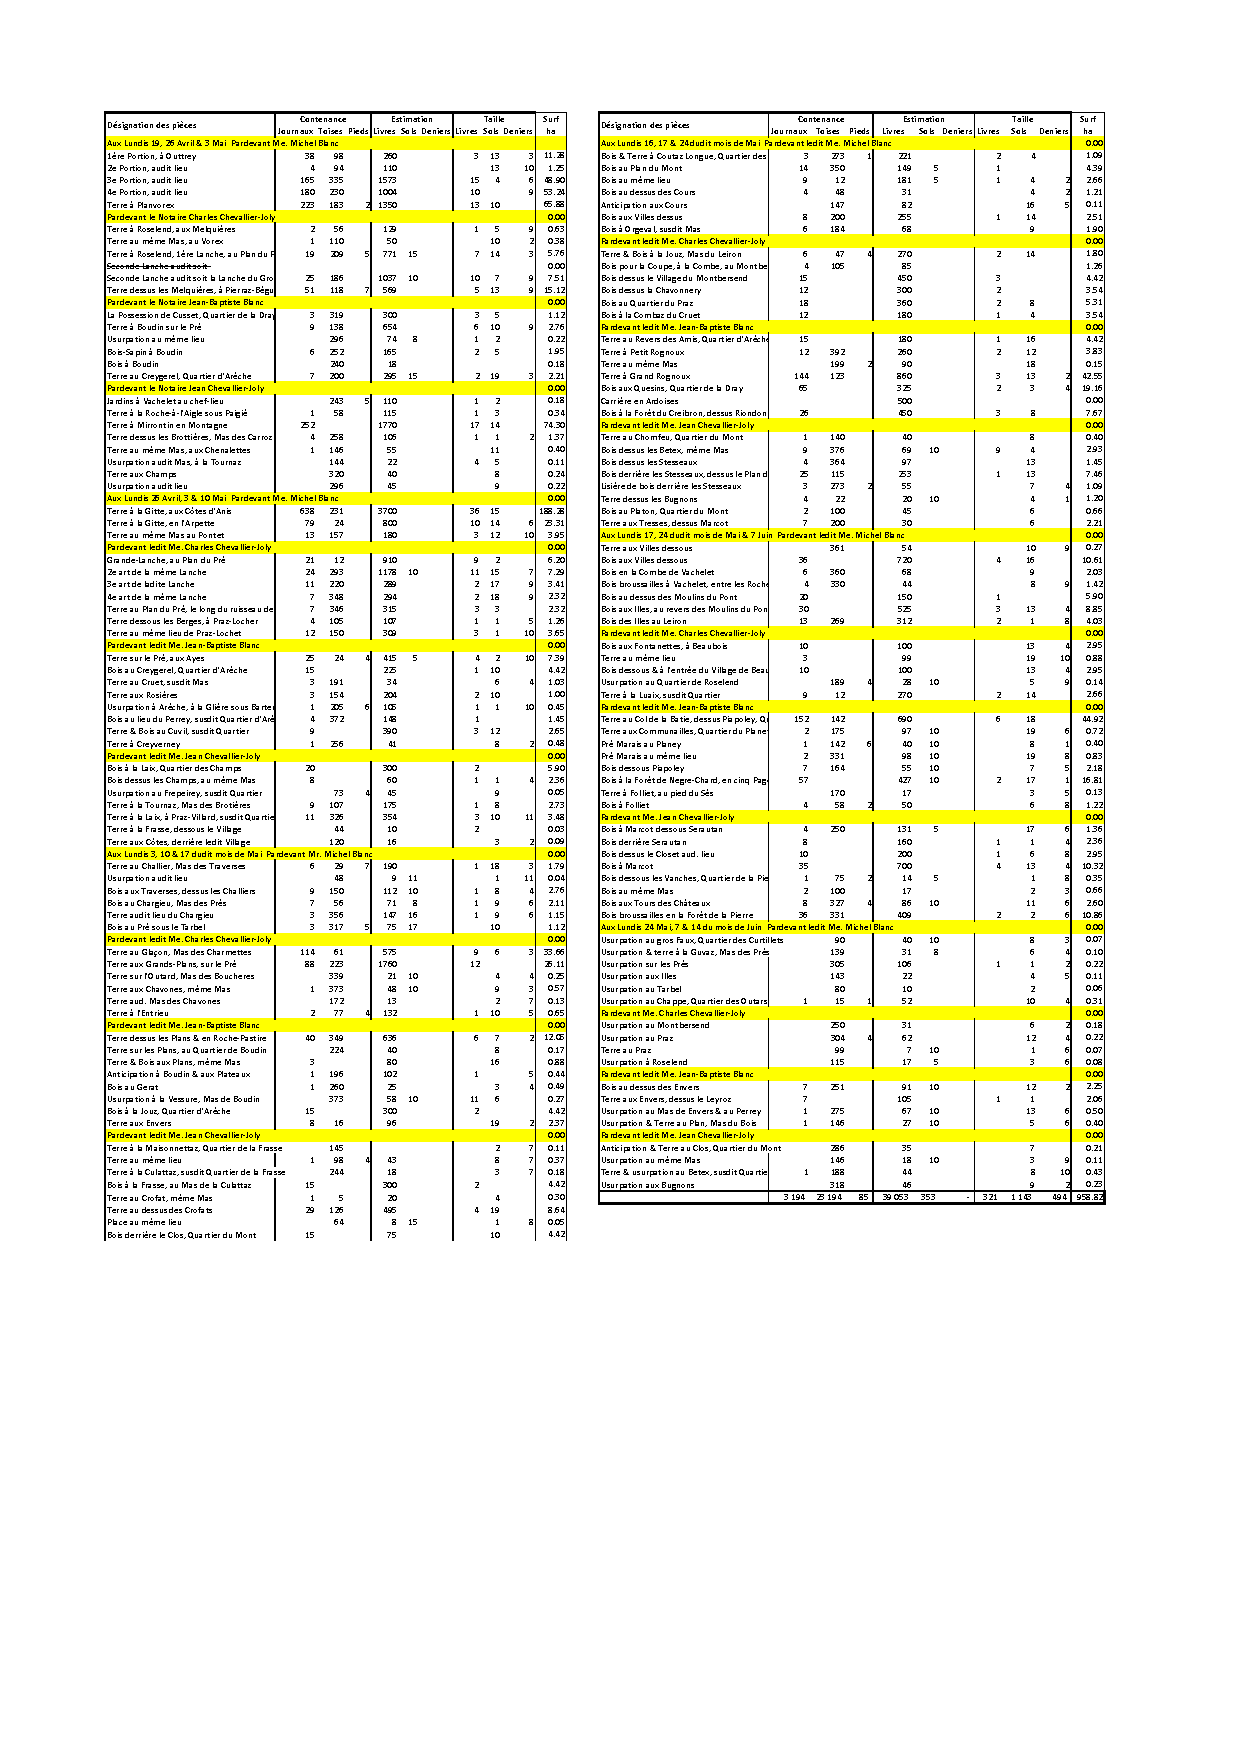
\includegraphics[ 
	width=1.3\textwidth, trim=1.7cm 8cm 0cm 1.5cm,
	 clip ]
	 {tables/4_Synthèse Manisfeste.pdf}
	\tabcaptionindex{tab:Manisfeste}{Liste des 151 Lots Vendus 1ier Manisfeste}
\end{table}
 Le manifeste recense 151 lots, regroupant 343 parcelles cadastrales. La superficie moyenne est d'environ 6 hectares par lot, mais cette valeur masque une forte dispersion. La majorité des lots (81\,\%) couvre moins de 5 hectares, tandis que quatorze seulement dépassant 12 hectares et représentent plus des deux tiers de la superficie vendue. 3/4 des superficies vendues sont des "Terres" contre 1/4 de Bois.

Les lots les plus importants correspondent tous à des pâturages d'altitude. 



Il ya a une certaine incohérence: il existe quelques très grands lots (dont un lot d'une contenance de 188ha) alors que le manifeste mentionne :
\begin{quote}
	«en exécution de ce que prescrit notre Ordonnance du second Juillet dernier, de ne pas prélever pour chaque Parcelle des contenances plus fortes de vingt journaux, à moins qu'il n'y ait des raisons particulières, dont on devra faire résulter dans les Verbaux\footcite[19]{1erManifeste}»
\end{quote}
(vingt journaux faisant 5.9ha)
\vspace{1em}
Cette observation est sans doute liée à la localisation des terrains retenus par le conseil, qui privilégie les espaces les plus éloignés et les moins fréquentés. Toutefois, le manifeste comprend également de nombreux lots de faible superficie, correspondant à des bois, jardins ou petites parcelles, ce qui montre que la vente ne concerne pas exclusivement de vastes alpages.

\begin{table}[htbp]
	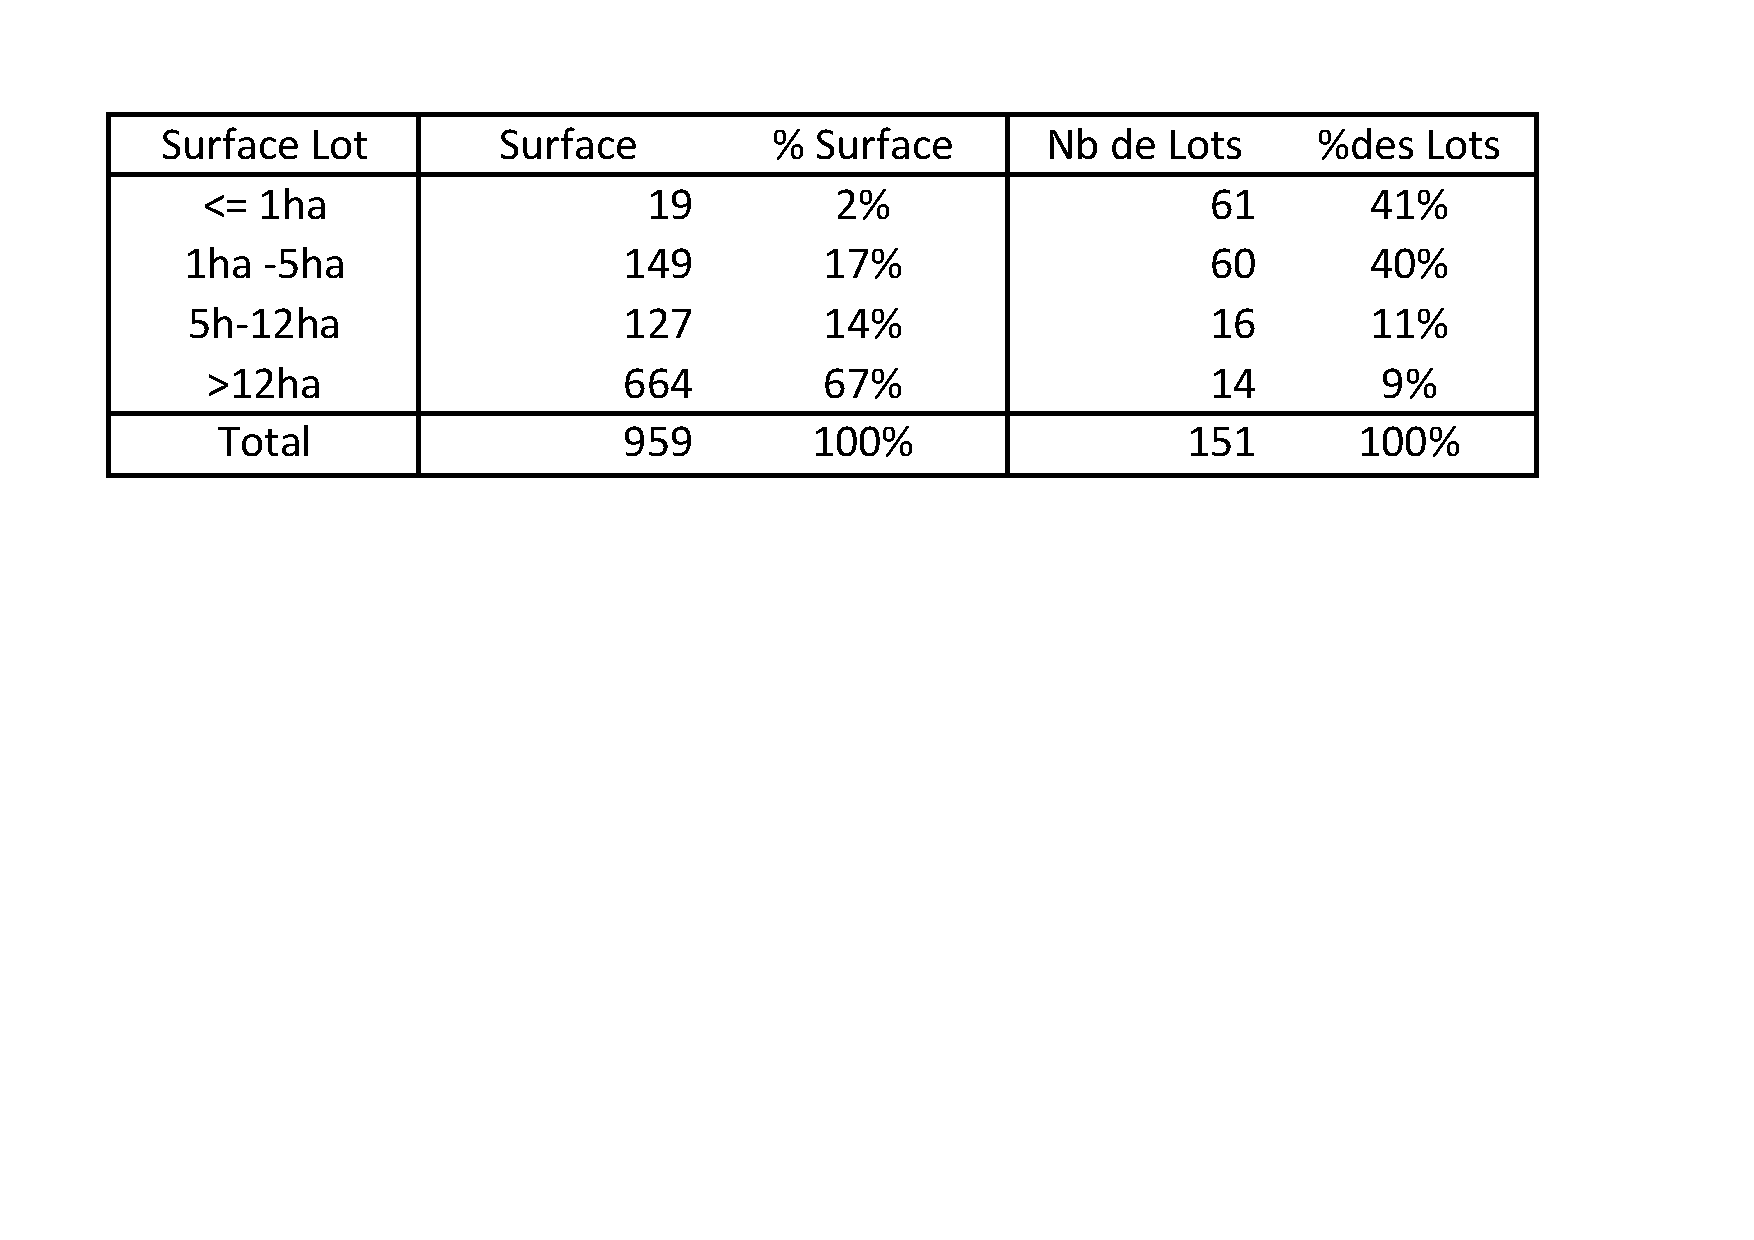
\includegraphics[ 
	width=\textwidth, trim=0cm 12cm 0cm 0cm,
	clip ]
	{tables/4_AnalyseManisfeste.pdf}
	\tabcaptionindex{tab:Tb_Manisfeste}{Répartition des Lots par surface}
\end{table}
L'analyse des correspondances entre lots et parcelles met en évidence que les limites des lots ne coïncident pas nécessairement avec celles du cadastre sarde. Si 98 lots ne comprennent qu'une seule parcelle et si 305 parcelles ne figurent que dans un seul lot, plusieurs grandes parcelles sont divisées entre plusieurs adjudications. Ainsi, la parcelle n\textsuperscript{o}~8725 (77 hectares) est répartie entre neuf lots différents, tandis que la parcelle n\textsuperscript{o}~11324 (381 hectares) est concernée par huit lots. Dans les deux cas, seule une partie de la parcelle est effectivement vendue, le reste demeurant dans le domaine communal.

Le manifeste distingue également deux types d'opérations. Cent vingt-cinq lots correspondent à de véritables ventes, tandis que vingt-six lots régularisent des occupations antérieures qualifiées d'« anticipation » ou d'« usurpation », concernant au total 51 parcelles.

Enfin, le document fournit, pour chaque lot, une estimation en livre. Ces estimations restent difficiles à interpréter (Les bois valent entre 25 et 100 Livres l'hectare). Elles donnent néanmoins quelques ordres de grandeur, par exemple 500 livres pour la carrière d'ardoise ou 110 livres pour un jardin d'environ 1\,800~m\textsuperscript{2} situé au chef-lieu.

\begin{landscape}
	\thispagestyle{empty}
	
	\begin{figure}[p]
		\centering
		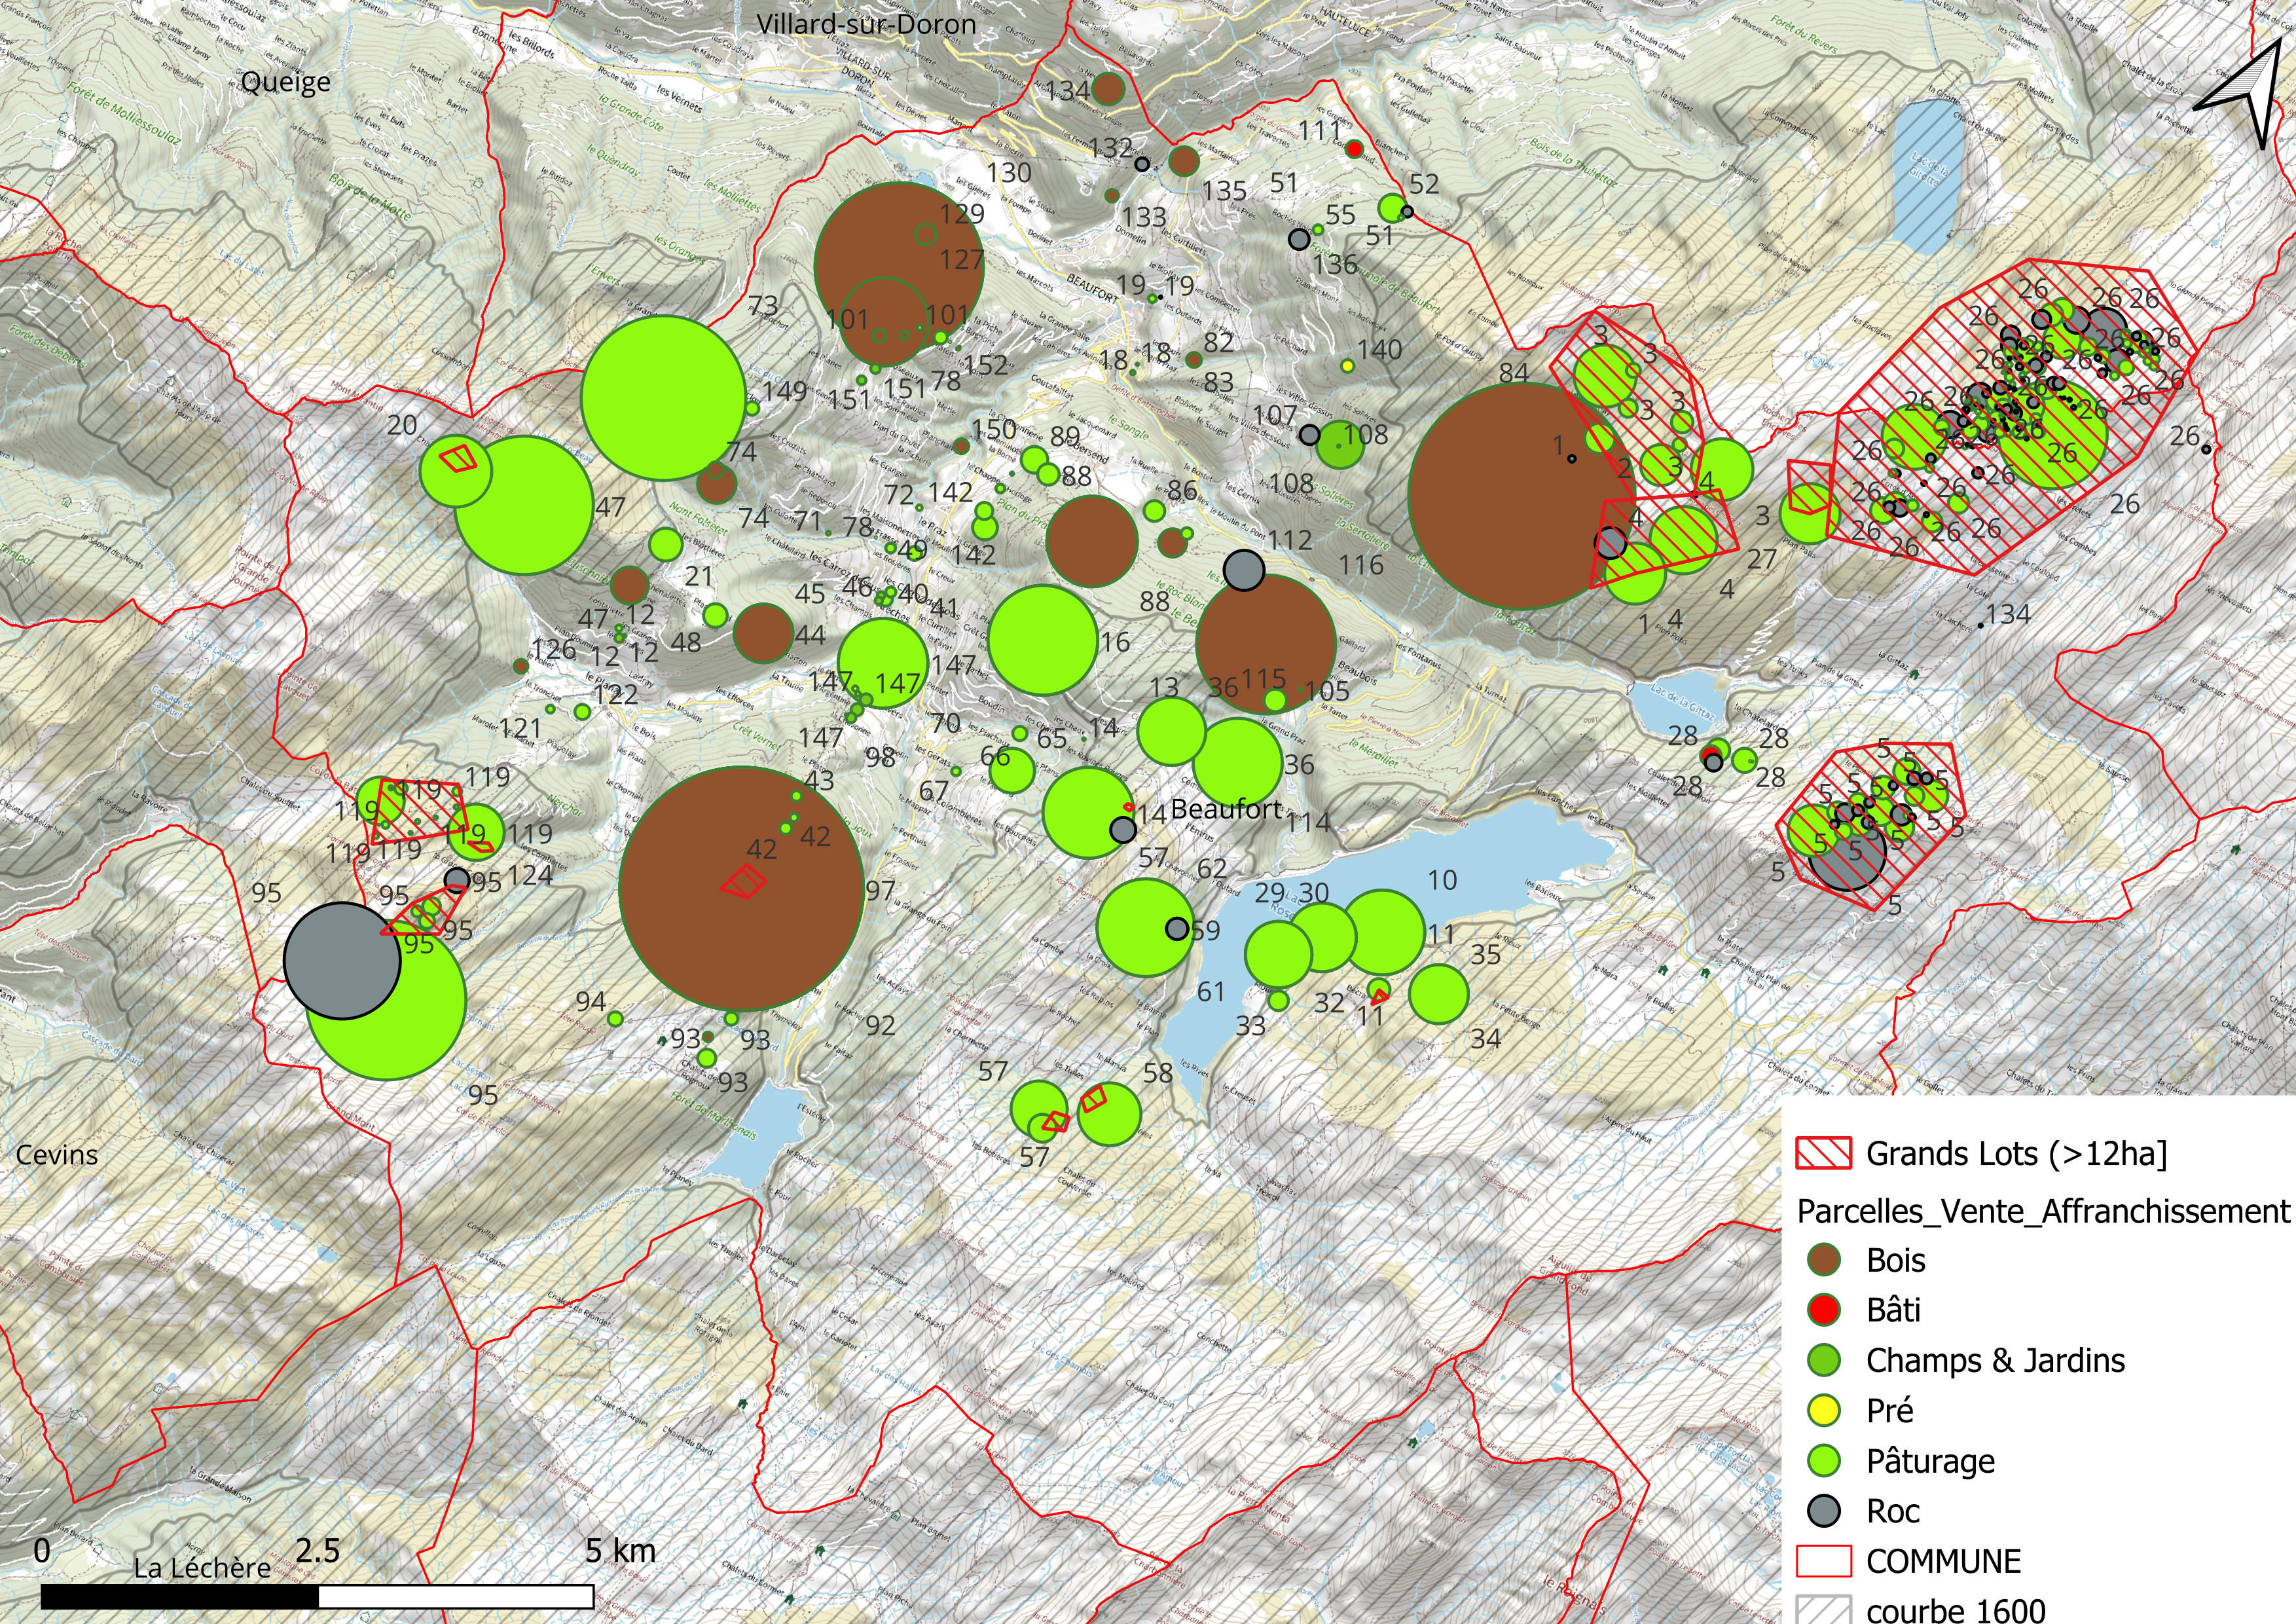
\includegraphics[
		width=\linewidth
		]{figures/4 Carte des Lots Ventes_Affranchissement.jpg}
		\caption{Carte des Parcelles par Lots}
		\label{fig:LotsAffranchissement}
		\idxcarte{Fig.~\thefigure{} -- Carte des Parcelles par Lots}
	\end{figure}
\end{landscape}
	
La carte de la figure~\ref{fig:LotsAffranchissement} permet enfin de visualiser la répartition spatiale des lots. Elle montre que les ventes concernent l'ensemble du territoire communal, même si les plus grandes superficies se situent logiquement dans les secteurs d'altitude où se concentrent les pâturages.

Au-delà des résultats propres à cette première campagne de vente, l'analyse du manifeste met en évidence les limites de la Mappe Sarde pour reconstituer les opérations d'aliénation des communaux. Le cadastre fournit un état parcellaire de référence, mais les lots constitués pour la vente obéissent à une logique différente. Ils peuvent regrouper plusieurs parcelles, n'en reprendre qu'une partie ou, au contraire, diviser une même parcelle entre plusieurs adjudications. Les limites des lots ne coïncident donc pas systématiquement avec celles du parcellaire cadastral: on voit alors le retour des descriptions paysagères et topographiques pour identifier un nouveau territoire

\chapter*{Conclusion}
\addcontentsline{toc}{chapter}{Conclusion}

L'étude de la communauté de Saint-Maxime de Beaufort confirme que, derrière les cadres juridiques de l'Ancien Régime, la société locale fonctionne déjà largement comme une société de classes. Si les trois ordres demeurent la référence institutionnelle du royaume, ils rendent imparfaitement compte des rapports sociaux observables dans cette communauté alpine. Les véritables distinctions opposent avant tout les grands propriétaires, souvent notaires, avocats ou bourgeois, à une paysannerie plus ou moins aisée, elle-même très différenciée selon l'importance des patrimoines fonciers.
Cette hiérarchie sociale ne paraît toutefois pas figée. Les actes notariés, les acquisitions foncières et les stratégies familiales suggèrent une certaine mobilité sociale. Plusieurs familles paysannes accèdent progressivement au rang des notables locaux, tandis que les patrimoines se recomposent continuellement par les mariages, les héritages et les achats.
Le patronyme Chevalier-Joly illustre bien cette porosité sociale : il apparaît à la fois dans le milieu notarial, à propos de l’affranchissement (cf Annexe, Maître Charles Chevallier-Joly chargé d'officier un certain nombre de vacations d'enchères), et dans le monde de l’exploitation pastorale (fermiers des Blanc, devenu indigent)évoqué par Hélène Viallet\footcite[264]{iallet1990Blanc}. L’exemple suggère moins une opposition simple entre notables et paysans qu’un continuum social, où certaines familles peuvent articuler propriété foncière, savoir juridique et exploitation des alpages.
\vspace{1em}
On peut tout de même s'interroger sur le conflit d'intérêt évident que pose le cumul des rôles de Me Joseph Blanc: son intérêt particulier rencontre d'un peu trop près l'intérêt général. Cependant, les réactions populaires contre les ventes de communs ne sont pas explicitement dirigées contre lui. Il est donc difficile de juger aujourd'hui sa situation très particulière.
\vspace{1em}

Cette fluidité sociale est sans doute favorisée par un niveau d'instruction exceptionnel. Près de 49\% des hommes sont capables de signer leur testament, proportion remarquable pour une communauté montagnarde du XVIIIe siècle. L'existence de plusieurs écoles, dont certaines sont gratuites et accueillent également les filles, témoigne d'un investissement ancien dans l'éducation. Cette diffusion de l'écrit a probablement contribué à faciliter l'accès aux fonctions juridiques, aux responsabilités communautaires et à la gestion des patrimoines.



Au terme de cette étude, La Mappe de 1738 ou la vente des communaux de 1768 suite à l'affranchissement des droits féodaux apparaît moins comme un objet d'étude isolé que comme des révélateurs du fonctionnement de la communauté de Saint-Maxime de Beaufort. L'analyse croisée des archives, de la Mappe Sarde et de leur exploitation dans un système d'information géographique met en lumière les logiques foncières, les stratégies familiales et les hiérarchies sociales qui structurent la communauté au XVIIIe siècle.

L'étude montre ainsi que les communaux constituent un observatoire privilégié de la société beaufortaine. Les choix opérés lors de leur aliénation révèlent non seulement la répartition des patrimoines, mais également les capacités différenciées des habitants à mobiliser des ressources financières, juridiques et relationnelles. Plus qu'un simple épisode de politique foncière, cette opération éclaire les mécanismes de fonctionnement d'une communauté montagnarde confrontée aux réformes de l'État sarde.

L'un des principaux enseignements de ce travail est également d'inviter à dépasser une lecture trop schématique de cette société. Les données réunies montrent une réalité plus nuancée que les oppositions traditionnellement avancées entre notables et paysans, grands et petits propriétaires ou investisseurs et exploitants. Les patrimoines sont souvent diversifiés, les situations intermédiaires nombreuses et les stratégies familiales complexes. Cette diversité invite à une certaine prudence dans l'interprétation des données cadastrales et rappelle que les catégories sociales demeurent poreuses.

La démarche mise en œuvre souligne également l'intérêt des outils numériques pour l'histoire rurale. Le géoréférencement de la Mappe Sarde, la reconstitution des parcelles et les analyses spatiales n'ont pas seulement permis de produire une nouvelle cartographie du territoire ; ils ont rendu possibles des questionnements difficilement envisageables à partir des seules sources manuscrites. La localisation des patrimoines, l'analyse des usages du sol en fonction de l'altitude, l'étude spatiale des acquisitions ou encore la mise en relation des patronymes avec les territoires illustrent les possibilités offertes par ces approches.

Ces résultats doivent toutefois être appréciés au regard des limites de la documentation. La Mappe Sarde ne constitue pas une photographie parfaite de la réalité foncière de 1768. Certaines incohérences de localisation, les imprécisions cadastrales, les modifications intervenues entre le levé du cadastre et la vente des communaux ainsi que l'impossibilité de reconstituer avec certitude les modes d'exploitation des parcelles imposent de conserver une grande prudence dans l'interprétation des résultats. Ces limites n'enlèvent rien à l'intérêt de la démarche ; elles rappellent au contraire la nécessité de croiser systématiquement les sources.
Il convient également de rappeler que la Mappe Sarde est avant tout un cadastre foncier. À ce titre, elle renseigne avec une grande précision la propriété, les usages du sol et les patrimoines immobiliers, mais demeure largement silencieuse sur d'autres composantes de l'économie locale. Les activités artisanales, les métiers du bâtiment, les activités commerciales ou encore les exploitations industrielles, telles que les mines ou les activités liées au bois, n'y apparaissent qu'indirectement, voire pas du tout. Seules quelques mentions ponctuelles, comme la mise aux enchères d'une carrière d'ardoise lors de la vente des communaux, permettent d'entrevoir ces secteurs d'activité. La société reconstituée dans cette étude est donc avant tout celle des propriétaires fonciers, même si ceux-ci pouvaient parallèlement exercer d'autres activités économiques qui échappent en grande partie à la documentation cadastrale.

Enfin, cette recherche ouvre plusieurs perspectives. La méthode développée pourrait être appliquée à d'autres communautés savoyardes disposant de la Mappe Sarde afin de comparer les structures foncières, les formes d'exploitation des espaces d'altitude ou encore les modalités d'appropriation des communaux. Une telle approche permettrait de replacer le cas de Beaufort dans une histoire plus large des sociétés alpines face aux réformes foncières et administratives du XVIIIe siècle.
	
	
	
	

\appendix

\chapter*{Annexes}
\addcontentsline{toc}{chapter}{Annexes}

\input{annexes/annexe_Affranchissement}
\input{annexes/annexe_Litige_Treicol}

\chapter{Méthodologie}

\maketitle

\section{Introduction}


\subsection{problèmes du nombre de parcelles}

Comme nous l’avons vu, le fichier Excel Barbéro contient 17803 parcelles.

Le numéro maximal attribué à la dernière parcelle répertoriée dans les documents de la Mappe de Beaufort aux ADS est : 17691.

Enfin le nombre de numéros de parcelles géoréférencées extraites des cartes Barbéro est seulement de 11787.

Une étape préalable consiste donc à comprendre ces différences.

a)	Nous avons constaté dans le fichier Beaufort-FICHIER-ATLAS-OK.xls qu’il manquait 136 numéros dans la séquence continue de 1 à 17691 ; en consultant les registres aux ADS, et en effectuant un sondage, il s’avère que ces numéros « manquants » y sont rayés et il est fait mention que ces parcelles ont été transférées  à la commune de « La Chapelle » à un moment donné durant l’élaboration de la Mappe ; « La vallée de Treicol est un secteur âprement disputé par Aime et les Chapelles, contre Saint-Maxime. Elle fait l’objet d’un procès pluriséculaire, puisqu’il débute en 1599 par le refus de Me Jean-François Dunand de payer la taille de sa montagne de Presset à Beaufort. L’affaire s’envenime, car de nombreux particuliers possèdent des alpages à Treicol. Pour être limitrophe de la vallée et augmenter ses prétentions, la communauté des Chapelles va jusqu’à acheter en 1732 une longue et étroite bande de rochers depuis la Pierre-Menta jusqu’à son territoire. Portée devant toutes les instances possibles, l’affaire n’est définitivement tranchée qu’en 1907, par un arrêt du Conseil d’État qui attribue la vallée à Beaufort.» 	\footcite{HViallet1993}.

La Chapelle est devenue la commune actuelle de la cote d’Aime (fusionnée en 2016 dans la Plagne Tarentaise). 

Carte9 : la zone « inconnu » correspond à l’information du « mas » des parcelles, ces parcelles n’étant pas référencées dans le fichier Excel Barbéro. 

Nous avons ajouté au fichier les 136 parcelles manquantes, ces lignes ne comportent aucun attribut descriptif.

b)	Autre particularité du fichier Excel Barbéro est qu’il contient :

-	Une parcelle non numérotée, mais avec la lettre « A » dans le champ n° de parcelle.

-	6 parcelles différentes, mais dont les numéros sont en doublon.


Récapitulatif :

Analyse des numéros 
du tb excel Barbéro	Tableau
Barbéro	Nb Entiers
+ Parcelles
manquantes	Hypothèses
Parcelles avec nb entier entre 1 et 17691	17552	17552	
Parcelles avec le même n° (nombre entier)	2	1	le doublon est une décimale omise
Parcelles manquantes (Transférées)		136	
Parcelle numérotée "A'	1	0	le n° omis est un nombre décimal
Parcelles avec un n° + une lettre	2	2	
Parcelles avec n° + lettre (n° déjà existant)	10		
Parcelles avec une décimale (1/2 ; 1/3,…)	232		
Parcelles avec le même n° nb + décimale)	4		
Total	17803	17691	

Conclusion : si nous totalisons uniquement les numéros avec un nombre entier, nous retombons sur le dernier numéro de parcelle (17691) des registres de la Mappe de Beaufort.


\subsection{Import de la Mappe dans QGIS}

La première étape \footnote{projet QGIS : Assemblage précis.qgz} a consisté à superposer à plat les différents éléments disponibles Cette approche évite à ce stade le  risque de déformation du fait d'un géoréférencement d'une carte ancienne sur une carte moderne IGN) : 

- calage les unes par rapport aux autres, les quatre images de la vue globale de la Mappe Sarde

- superposition par-dessus (avec l'outil Georeférencer de QGIS) les 45 photos détaillées de la Mappe téléchargées des ADS. 



\cartefigure
{figures/1 MS 45 photos détails non GeoRef.jpg}
{fig:MS45nonGeoRef}
{45 photos assemblées de la Mappe Sarde de Beaufort}

\cartefigure
{figures/1 Assemblage des 45 photos détail Mappe Sarde Beaufort.jpg}
{fig:MS45Assemblage}
{assemblage des 45 photos de la Mappe Sarde de Beaufort}

Remarques :\\
- une photo est manquante sur le site des ADS (\texttt{361\_b\_16}). Afin de la constituer, nous avons découpé un morceau de  la photo globale associée . Bien évidemment la qualité est beaucoup plus faible.

- Le collage des 45 photos a fait apparaître quelques non-recouvrements du fait du photographe des ADS

- la Mappe Sarde de Beaufort est parfois très abîmée en particulier la jonction entre les deux toiles peintes est impossible du fait des manques.

\cartefigure
{figures/1 MS 45 photos détails Anomalies.jpg}
{fig:MS45_Anomalies}
{photos 361_013 et 014 non jointives avec 019 et 020}






\subsection{Retraitement des cartes Barbéro}

Le CD-Rom fournit 55 images-cartes comme celle-ci :

\cartefigure[0.5\textwidth]
{figures/1 exemple carte CD Barbéro.JPG}
{fig:BarberoCarte01}
{exemple Carte 01 CD Barbéro} 

Telle quel, ces cartes-images, ne sont pas plus exploitable que les photos de la Mappe déjà importées.
En revanche, elles contiennent deux éléments seulement : des lignes et des chiffres.

Des outils permettent des retraitements suffisamment automatiques pour rendre possible une alternative au travail manuel sur les 55 images et les 17691 parcelles. Le détail des outils et des étapes est décrit en annexe (cf Annexe3), en voici les tâches principales :

-	Détourage des 55 photos pour ne garder que les lignes et les numéros

-	Séparation des figures : 55 images avec seulement les contours des parcelles et 55 images avec les numéros des parcelles seulement .

\cartefigure[0.5\textwidth]
{figures/1 Beaufort secteur 01 original.jpg}
{fig:BarberoCarteNumOnly}
{Détourage et conservation des numéros exemple Carte 01}


\cartefigure[0.5\textwidth]
{figures/1 Beaufort secteur 01 reds.jpg}
{fig:BarberoCarteRed}
{Détourage et conservation des contours des parcelles exemple Carte 01}



-	Décodage des chiffres, les outils d’OCR que nous avons essayés ne donnant pas de résultat, nous avons dû coder en python une reconnaissance de formes au niveau pixel ; chaque un des nombres (0 à 9) ayant plus ou moins une signature en pixel unique.

-	Nous avons gardé la position des ensembles de pixels composant chaque chiffre. Puis nous avons regroupé les chiffres mitoyens pour aboutir a) à un nombre = au numéro de la parcelle et b) une référence (X,Y) du pixel au centre du groupe de chiffre composant un nombre.

-	Un retraitement manuel sur une centaine de nombres non reconnus a été nécessaire : nombre tronqué en bordure d’image, nombre mélangé à des éléments superposés comme la boussole ou la barre d’échelle ou encore chiffre mal pixélisé non reconnu dans le traitement précédent.

Au final de cette étape nous obtenons :

-	55 images des contours de parcelles 

- 	55 images des numéros (images inutilisées sauf pour vérification)

-	55 tables avec les nombres reconnus et leur position pixel (X,Y) sur chaque image.

Les 3 ensembles sont exactement superposables

Nous avons rassemblé les 55 tables en un seul fichier \texttt{XY\_No\_Parc.csv} (fichier ; X ; Y ; No\_Parc) et nous avons éliminé les doublons (parcelle se trouvant affichée sur deux images de secteur mitoyen). Au final nous avons 11.744 numéros distincts reconnus. Ce nombre représente les 2/3 (66\%) des 17.803 parcelles référencées dans la table Barbéro.

C'est assez compréhensible : la table Barbéro (fichier Excel) est issue des registres associés à la Mappe alors que les numéros sur les cartes sont issus de la lecture de la carte elle-même où les numéros ne sont pas toujours lisibles.

Nous verrons comment localiser approximativement les parcelles du tiers restant avec une méthode fondée sur la localisation du Mas de chaque parcelle. 




\section{Attribution d’une altitude à chaque parcelle}

\subsection{Géoréférencement des cartes Barbéro}

Le CD-Rom contient une carte d’assemblage des 55 secteurs :


\cartefigure 
{figures/1 Tableau d'assemblage des secteurs.JPG}
{fig:BarberoAssemblage}
{Carte d'assemblages de cartes fournie dans le CD Barbéro}


En utilisant la fonction géoréférencement de QGIS, nous avons superposé les 55 images des contours des parcelles sur l’assemblage détaillé de la Mappe. Cette opération était relativement simple (mais longue !) puisque nous pouvons assez facilement faire correspondre des points de ce géoréférencement en retrouvant les lignes des parcelles des cartes Barbéro avec celles correspondantes de la Mappe.

Malheureusement dans un ou deux cas l’assemblage des cartes Barbéro comportait des lacunes (certaines cartes ne se superposaient pas). C’est dommage, mais l’impact est resté très marginal.

Ensuite, nous avons réutilisé les mêmes points de géoréférencement de l’étape précédente, pour géoréférencer les cartes des numéros de parcelles, afin que chaque numéro se retrouve au bon endroit.

À ce stade, nous avons 3 couches superposées avec :\\
- les photos détaillées de la Mappe\\
- les contours des parcelles\\
- les numéros (en mode image, inexploitables mais utile pour vérifications ultérieures)


La dernière étape a consisté à transformer la table des numéros de parcelles en une couche vectorielle avec une table d’attributs obtenant ainsi la géolocalisation des numéros de parcelles.

un programme python qui : \\
- prend chaque la table "i"\\
- la charge en layer vecteur (add delimited text)\\
- l'exporte en fichier gpkg (format de couche vectorielle de QGIS)\\
-charge ce fichier dans le GeoRefrencer de QGIS et l'associe au fichier des points utilisé pour géolocaliser les contour des parcelles\\
- lance le géoréférencement

Au final nous avons 55 fichiers gpkg qui se superposent aux trois couches raster précédentes.

Pour chacune des couches je fusionne tous les éléments en un seul :\\
- les 45 images raster de la Mappe en un raster virtuel : \texttt{Virtual photo detaillées.vrt} \\
- les 55 images des contours des parcelles en un raster virtuel \texttt{Virtual_Red.vrt}\\
- les 55 fichiers gpkg des numéros de parcelles en un seul gpqk  \texttt{text}\\

Remarque : il y a dans le fichier des numéros de parcelles des numéros en double (ou triple et même quadruple. Ce sont sans doute des numéros qui apparaissent sur plusieurs secteurs Barbero (les secteurs se chevauchent) mais il y a peut-être d'autres anomalies. Nous avons éliminé tous les doublons à moins de 100m les uns des autres. Il reste 35 anomalies de doublons éloignés l'un de l'autre. Il s'agit sans doute de reconnaissance erronée des numéros sur la photo de la Mappe par D. Barbero (exemple sur le secteur 44 une parcelle est lisible sur la carte comme la numéro 16875 mais elle est transcrit par sur par D.Barbero en 6871), l'autre explication possible une reconnaissance erronée des numéros sur les images Barbero par notre programme de retranscription.




Le décodage numéros de parcelles à partir des cartes de secteur Barbéro a abouti à reconnaître 11787 numéros de parcelles (et à les géoréférencer).

Les deux tables, celle du fichier excel du CD-Rom (enrichie par notre modélisation) et celle issue du géoréférencement des numéros de parcelles ont un index commun qui est le numéro de parcelle (dans quelques cas, une dizaine, une lettre est associée au numéro d'une parcelle, dans ce cas une décimale a été ajoutée au numéro de la parcelle par exemple la parcelle 17301 A a été numérotée 17301.02 cette décimale permet de ne pas confondre avec les décimales de 0.5 pour 1/2 et 0.33 pour 1/3 ). 

En fusionnant les deux fichiers, il est donc aisé de créer une seule carte vectorielle avec des données attributaires pour toutes les parcelles et une géolocalisation pour les 2/3 d'entre elles.

Mais il manque 6016 parcelles non géoréférencées, ce qui représente tout de même un tiers des parcelles.

Nous ne savons quels ont été les moyens et méthodes de Dominique Barbéro pour faire son travail de cartographie: Est-ce parce qu’il n’a pas pu lire certains numéros sur la Mappe originale ? Est-ce seulement l’édition des images de secteurs qui n’a pas affiché tous les numéros et toutes les parcelles ?

Toujours est-il que la proportion de parcelles non référencées pose un vrai problème pour l’objectif de cette étude qui est d’isoler les parcelles d’altitude.

\subsection{Geolocalisation précise sur carte Ign}

Nos trois couches :  photo de la Mappe (Raster), contour parcelle (Raster) et Parcelles Barbéro (vecteur), se superposent parfaitement.

Nous avons alors géoréférencé précisément la Mappe,  sur un fond de carte IGN en utilisant une variété de points de calage : \\
- les contours de la commune (en particulier les angles )\\
- les églises, chapelles, village...\\
- les cours d'eau\\
puis nous avons réutilisé ces points de calage pour géoréférencer les contours de parcelles et surtout la couche des parcelles.

\cartefigure
{figures/1 Mappe de Beaufort Georéférencée sur IGN.jpg}
{fig:MSsurIGN}
{Mappe de Beaufort Georéférencée sur IGN}

Le résultat est tout à fait satisfaisant, dans le sens où il n'y a pas de déformation exagérée de la Mappe de Beaufort quand on la transforme pour qu'elle se cale sur la carte moderne IGN

\subsection{Geolocalisation des parcelles manquantes}

Il reste, à ce stade 6016 parcelles non géoréférencées, mais nous connaissons les mas où elles se situent.

Les mas sont des territoires à l’intérieur du territoire de Beaufort, pour la plupart il s’agit d’un hameau ou groupement de maisons et les parcelles qui en dépendent, autrement ce sont des lieux dits. Toujours est-il que toutes les parcelles (le 17803) sont associées avec un « mas » et un seul.

Le CD-Rom Barbéro contenait une carte des mas, mais nous avons préféré reconstituer nous-mêmes les mas avec l'outil cartographique QGIS.

Nous avons donc créé une couche vectorielle des Mas, en créant des polygones qui entourent toutes les parcelles déjà géoréférencées.

Ce faisant nous avons constaté un certain nombre d'anomalies, en particulier des ensembles disjoints d'un même mas.

Nous avons alors créé un attribut "Mas2" qui est égale à "Mas" sauf dans certain cas, par exemple nous avons crée "Acrays 2" , "Ban 2", "Curtillet ?", "Dommellin ?", "Isle et Lacura ?", "Pecherie", "Plan ou Plains ?", "Praz" et "Territoire transféré à LaChapelle". Le principe était de n'avoir que pour chaque mas (Mas2) un territoire homogène.

\cartefigure
{figures/1 Carte des Mas.jpg}
{fig:Mas2}
{Carte des Mas reconstitués}

xxxxxxxxxxxxxxxx cas des parcelles hors de leur mas xxxxxxxxxxxx



\subsection{Ajout de l'altitude des parcelles}

Les cartes IGN fournissent aussi des couches de courbes de niveau, permettant de déterminer l'altitude de chaque point. Nous avons donc ajouté deux informations à la table attributaire des parcelles : l' altitude et une tranche d'altitude : \texttt{ [inf à 800m], [800-1000m], [1000-1200m], [1200-1400m], [1400-1600m], [1600-1800m] et [sup à 1800m]}.

Nous avons aussi ajouté une couche matérialisant les zones où l'altitude est supérieure à 1600m.

Il n’y a pas de définition précise des zones d’alpages par rapport aux zones d’hivernage permanent ou aux zones de pré-alpages. Dans le système agropastoral dit de « grande montagne » \footcite{ArbosMouthon2017} \footcite{Arbos1922}, il s’agit des pâturages utilisés entre la Saint XXX et le 24  juin (fête de la Saint Jean-Baptiste) et le 12 septembre (fête de la Saint XXX). 

Nous savons qu’à la fin de l’été, les grands troupeaux sont démantelés et dispersés dans des chalets capables de loger entre 5 et 10 vaches. Les vaches des grands troupeaux d’alpage pouvant appartenir soit au propriétaire (ou tenancier) de l’alpage soit au propriétaire (« client » de l’alpagiste) du chalet d’hivernage.

Suivant la richesse (en terre) des paysans, ils pouvaient posséder 3, 4 … 6 chalets intermédiaires entre la zone estivale et la zone d’hivernage finale en bas de vallée.

L’architecture des chalets varie en fonction de leur utilisation. Il est facile en se promenant dans la vallée du Beaufortain d’identifier à quelle altitude, les chalets d’hivernage disparaissent et sont remplacés par des granges, sans étable ni fenêtre ni espace d’habitation permanente. Par ailleurs une partie non négligeable des vieux chalets datent du 18e siècle. 

Cette approche empirique nous a conduits à fixer à 1600m l’altitude au-delà de laquelle on peut parler d’alpage. Nous avons identifié les derniers chalets d’habitat permanent à 1500m mais nous avons supposé que les prés ou pâturages avoisinant ces chalets étaient utilisés pour récolter le foin pour passer l’hiver et non pour la grande pâture.

Cette hypothèse est confirmée par l’exploitation actuelle des alpages, bien qu’il faudrait aussi prendre en compte l’histoire du climat. Le XVIIIe siècle était nettement plus froid qu’au XXe siècle où s’est mis en place l’agropastoralisme sous sa forme actuelle. Par conséquent la marge de 100m par rapport aux dernières habitations permanentes nous paraît aussi légitime de ce point de vue.




\subsection{Point d'étape : toutes les parcelles sont situées géographiquement}

Jusqu'à présent, le travail fut très technique, long et parfois fastidieux, mais cela nous a permis d'obtenir enfin une base de travail utilisable en Histoire.

Remarque : ce travail est déjà fait et disponible en ligne pour les communes de Hautes Savoie par les Archives Départementales de Haute-Savoie. Pour la Savoie, il est fait partiellement (CD Barbéro) et sur un nombre de communes limité. Sur la vallée du Beaufortain, seule la commune de Beaufort a été traitée au format Barbéro, rien n'est disponible pour les communes de Queige, Villard-sur-Doron et Hauteluce en dehors des documents d'origine de la Mappe. 


A ce stade nous avons donc une nouvelle table reprenant toutes les informations de la table initiale du CD Barbéro avec en plus pour chaque parcelle :\\
- son géoréférencement \\
- son altitude et sa classe d'altitude\\
- son occupation du sol plus utilisable que l'attribut nature du sol\\
- sa surface en ha (déduite de celle en m²)\\
- son mas (mas2) retravaillé pour n'avoir que des territoires d'un seul bloc \\
- des informations plus techniques comme le nom du secteur Barbéro sur lequel se situe la parcelle et ses coordonnées en pixel, et pour les parcelles n'en faisant pas partie la méthode qui a permis de les placer par rapport aux autres)



\section{Constitution d'une base de données enrichie}

Afin de rendre possible l'exploitation historique du cadastre, les données initiales ont été complétées par plusieurs informations nouvelles.

Les graphies manifestement variantes d'un même mas ont été harmonisées afin de constituer des ensembles territoriaux cohérents. Un attribut \texttt{Mas2} a ainsi été créé pour faciliter les traitements statistiques et cartographiques.

Les nombreuses dénominations cadastrales de la rubrique « Nature » ont également été regroupées dans une nomenclature simplifiée d'occupation du sol. Cette opération avait pour objectif de conserver la richesse descriptive des registres tout en permettant une lecture synthétique de l'organisation du territoire.

Enfin, chaque parcelle a été associée à une altitude obtenue par croisement avec un modèle numérique de terrain. Des classes altitudinales ont ensuite été définies afin de permettre l'étude de la répartition des propriétés, des usages du sol et des formes d'exploitation selon l'altitude.

\section{Résultat obtenu}

À l'issue de ce travail, chaque parcelle dispose :

\begin{itemize}
	\item des informations cadastrales issues des registres sardes ;
	\item d'une localisation géographique ;
	\item d'une appartenance à un mas ;
	\item d'une catégorie homogène d'occupation du sol ;
	\item d'une altitude et d'une classe altitudinale ;
	\item d'une superficie exprimée en hectares.
\end{itemize}

Cette base de données constitue le corpus utilisé dans l'ensemble des analyses présentées dans les chapitres suivants.

Les traitements techniques ayant permis la constitution de ce corpus sont présentés en détail dans l'annexe méthodologique.

\section{Méthodologie}

\subsection{Analyse de la table du CD-Rom : numérotation des parcelles}

Le CD-Rom Barbéro contient un ficher Excel : Beaufort-FICHIER-ATLAS-OK.xls contenant 17803 parcelles  (avec en plus, une ligne d’en-têtes des colonnes) :

•	Numéro : il s’agit des numéros de parcelles a priori numériques dont le plus grand numéro est 17691. Il devrait a priori avoir 17691 parcelles sur la commune de Beaufort du Cadastre Sarde mais on constate immédiatement que le nombre de lignes ne correspond pas au nombre de parcelles

•	CF : Chef-lieu « O » ou « null » ; signification à investiguer ultérieurement

•	E : Ancien fond ecclésiastique « O » ou « null » ; signification à investiguer ultérieurement

•	I : « O » ou « null » ; signification à investiguer ultérieurement (dans la notice livrée avec le CD-Rom il est fait mention à cet emplacement d’une colonne nommée « N » (pour Noble)

•	Propriétaires : nous avons là des noms et prénoms des propriétaires avec parfois des compléments d’information par exemple « MONOD Jeanne soit Popelin veuve d'Antoine GACHET » ou « TARIN Nicolas et Humbert son frère» et aussi des noms de communautés par exemple « La communauté pour l'usage commun » ou « Chapelle de Roselend »

•	Statut : cette colonne contient du texte avec des valeurs répété : « Bourgeois » « communier » … il s’agit d’une information sur le statut du propriétaire a priori tel qu’il est inscrit sur le registre associé au cadastre

•	IND : parcelle en indivision, elle contient des valeurs « null » et quelque « O »

•	Mas : 

•	Nature : cette colonne contient du texte avec des valeurs récurrentes : « Roc », « Pâturage » ; « Marais et pâturage » … qui sont des descriptions de la nature du sol

•	DB : cette colonne contient des valeurs numériques 0, 1 , 2 ou 3 qui correspond aux quatre « degrés de bonté ». Le degré de bonté est une évaluation de la qualité (ou du rendement) du sol, faite par les agents du duché de Savoie en charge du relevé du cadastre, il a un but fiscal

•	m² : il s’agit sans doute de la surface de la parcelle en m² ; le registre du cadastre contenant de valeur de superficie selon une double mesure : la mesure de Savoie (Journaux, toises, pieds) et mesure de Piémont (Journaux, Tables, Pieds). 1 journal de Savoie équivaut à 0,3685 ha, celui du Piémont lui est légèrement supérieur. Cette conversion a été réalisée sans doute par le créateur du fichier D.BARBERO. (remarque : l’ensemble de la commune actuelle couvre 149,53 klm²  mais la partie transférée à l’époque de l’établissement de la Mappe Sarde est revenue à la commune actuelle de Beaufort sur Doron, la somme des surfaces du fichier D.BARBERO est égale à 139.648.325 m² soit 139,6 klm² ce qui est cohérent, on peut donc valider que la surface sur fichier Excel est en m² d'autant plus qu'à l'époque de l'établissement de la Mappe une partie des parcelles a été rayée car réattribuée à la paroisse de LaChapelle, elles ont été depuis réintégrées à la commune de Beaufort, dont il est normal que la superficie calculée par Barbéro soit inférieure à la superficie de la commune actuelle de Beaufort-sur-Doron) 

•	Avoine : des valeurs null ou numérique s’étalant de 13,5 à 22

•	Seigle : des valeurs null ou numérique s’étalant de 0,5 à 4 (les valeurs 0,5 sont stockées au format texte « 1 / 2 » nous les avons changées en 0,5

•	F. Bœuf : sous bœuf est regroupé le nombre de bovins, la colonne contient des valeurs numériques de 0,5 à 9 puis pour les valeurs supérieures le nombre est suivi de la lettre « L » : « 10 L », « 12 L », « 100 L » …

•	F. Cheval : sous Cheval est regroupé le nombre d’équidés de toute sorte (âne, mule, mulet cheval ) . La colonne contient des valeurs numériques de 0,5 à 9 puis pour les valeurs supérieures le nombre est suivi de la lettre « L » : « 10 L », « 12 L », « 100 L » …

•	Fascines : (fagot de petit bois ?) valeur numérique non investiguée pour l’instant

•	Chevron : valeur numérique sans doute bois d'œuvre pour charpente

•	Latte : valeur numérique sans doute bois d'œuvre pour des planches

•	Pièce 1 : valeur numérique non investiguée pour l’instant

•	Pièce 2 : valeur numérique non investiguée pour l’instant

•	N° Grief : champs pouvant contenir une ou plusieurs valeurs numériques, il s’agit de numéro de référence des contestations faites auprès des autorités relativement à la parcelle cadastrée. En principe il faudrait normaliser ce champ et créer une logique de relation 1-n entre une parcelle et les griefs associés, cependant il n’y a que 22 cas où une parcelle est associée à 2 ou 3 griefs, et l’étude des griefs est très secondaire dans notre étude.

•	Grief : champ texte contenant une typologie selon les types de griefs

•	Problèmes : descriptif sommaire du grief


Degré de Bonté :

Dans l’attribution des degrés de bonté, chaque type d’occupation du sol comporte les trois classes ; la qualité de la parcelle pouvant être bonne (1), moyenne (2) ou mauvaise (3). Par exemple pour la paroisse de Landry en vallée de Tarentaise (Savoie) la « note des estimes en degré avec leurs catégories… » nous informe sur la production qu’un terrain doit fournir pour se voir attribuer tel ou tel degré de bonté. Un pâturage doit produire annuellement deux quintaux de foin pour obtenir le degré de bonté 1, un quintal et demi pour le 2 et un quintal pour le 3. Pour les champs, la mesure est en bichet et il en faut vingt-neuf répartis en froment, seigle et farine pour répondre aux critères du degré de bonté 1, vingt-six pour le 2 et vingt-trois pour le 3, et ainsi de suite pour chaque usage du sol. Pour le bâti, les estimateurs attribuent le degré de bonté d’une terre voisine, de préférence appartenant au même propriétaire. Cette méthode d’évaluation des terrains fixe des niveaux d’exigence précis basés sur le rendement de la parcelle. Ainsi, les parcelles classées en 1 sont de bonnes terres productives, car les critères exigés pour avoir ce degré de bonté sont du même niveau. Le fait que chaque nature de sol comporte l’intégralité des classes (1, 2 et 3) et que les critères d’évaluation répondent à un même niveau d’exigence permet une comparaison entre deux terrains du même degré de bonté. \footcite{Baud2010} 


Mesure de Savoie :
« La base de ce système est le « pied de chambre de 0,033m qui élevé au carré donne le « pied de cadastre de 0.92m². un carré de 8 pieds forme la toise carrée (7.370m²) et 400 toises carrées équivalent à un journal de Savoie dont la valeur exacte est de 29.4838 ares. On compte pour les approximations 3 journaux à l’hectare » 	\footcite{GUICHONNET1955}


Mesure de Piemont :

« Les cadastreurs piémontais se servirent des unités de leur pays et qui dérivaient du pied liprand de 0,513 m. Il fallait 6 pieds pour faire un trabuc (3,082 m) et 2 trabucs pour une perche (6,164 m). Ces mesures linéaires servaient de base aux unités agraires suivantes : le pied de table (rectangle de 1 x12 pieds liprands de côté) ou 3,167 m². La table, ou perche carrée vaut 12 pieds de table (38,009 m) et 100 tables, ou 400 trabucs carrés, donnent un journal de Piémont. La mesure de Piémont est à préférer lorsqu’on utilise l’ancien cadastre. Pour les usagers soucieux de l’exactitude des contenances, elle est évidemment meilleure car elle résulte des opérations sur le terrain ; pour l’historien, elle est commode car la conversion des tables en journaux repose sur la base 100. » Idem


Mas :

«On a la preuve, par les reconnais; féodales, que les mas sont antérieurs de trois ou quatre siècles au cadastre, et que les « trabucants » piémontais n’ont fait qu’enregistrer un état de fait profondément et obscurément enraciné dans la tradition paysanne. Les mas appartiennent à plusieurs propriétaires, nobles ou roturiers, et le régime foncier de 1730 recouvre une réalité agraire très antérieure; ils chevauchent parfois plusieurs communes et ne portent pas toujours le nom des villages ou des lieux-dits qu’ils renferment, mais un toponyme d’étymologie romaine ou germanique. Leur étendue comprend rarement une seule zone de végétation, mais englobe différents types de terroirs et semble bien représenter une unité élémentaire d'exploitation, domaine d’un seul individu. » Idem p296

a) Nettoyage des données

•	Pb colonne « Numero »

En fin de fichier il y a 13 lignes avec des valeurs alphanumériques : 12 parcelles ont une lettre à la suite du numéro de parcelle et 1 parcelle a une lettre sans numéro :

17160 B;;;;BOUCHAGE Jean Baptiste;..\\
17161 A;;;;BUGAND Claude;… \\
17301 A;;;;MARTIN Claude;… \\
17302 B;;;;MARTIN Claude;… \\
17303 C;;;;La communauté pour l'usage commun;Communaux;… \\
17304 D;;;;La communauté pour l'usage Commun ;Communaux ;… \\
17305 E;;;;La communauté pour l'usage commun;Communaux;…\\
17306 F;;;;La communauté pour l'usage commun;Communaux;… \\
17307 G;;;;La communauté pour l'usage commun;… \\
17308 H;;;;La communauté pour l'usage commun;…\\
17309 I;;;;La communauté pour l'usage commun;\\
17310 K;;;;La communauté pour l'usage commun;\\
A;;;;TOCCAT Daniel;Communier;;;;3;1543;;;;;;;;;;;;\\

Nous avons créé une nouvelle colonne : Complément_numéro.

Les lettres des 13 lignes sont déplacées dans cette nouvelle colonne, et la ligne sans numéro se voit attribuer un numéro « 0 ».

Il y a aussi des parcelles dont le numéro est suivi de 1/2 , 1/3 ou 1/4 , ces valeurs ont été remplacées par des décimales (0.5, 0.3, 0.25) ajoutées au numéro de parcelle.

Il reste à comprendre pourquoi le nombre de lignes est significativement différent de la valeur maximum de numéro de parcelle. Mais nous allons d’abord importer ce fichier dans une base de données de travail.

•	Pb colonnes « CF » , « E », « I » , « IND »

Les valeurs « O » dans les colonnes « CF » , « E », « I » , « IND » ont été remplacées par des « Oui » afin de permettre une caractérisation booléenne.

•	Pb colonne « m² »

147 ;;;;VIALLET Jacques fils de Benoit;Communier;;Praz;Chenevier;1;\#VALUE!;21;3;;;;;;;;;;\\
La valeur \#value est remplacé par la valeur « null » \\
•	Pb colonne « Nature »

La colonne Nature est longue et contient beaucoup de double description, par exemple « bois et pâturage » ou « prés et teppes », une option de normalisation aurait été de décomposer en une relation 1-N : une parcelle pouvant être reliée alors à deux natures « bois et « pâturage » ; mais n’étant pas certain de comprendre précisément l’intention du géomètre-cadastreur, nous avons pris l’option de laisser pour l’instant le champ nature tel quel, mais en revanche de créer un concept « Occupation_Sol » pour regrouper les nombreuses « Natures » en ensemble homogène en prenant pour principe lorsqu’une Nature est « multiple » de prendre la première comme la Nature principale ; par exemple « « bois et pâturage » » aura la valeur « Bois » pour « Occupation_Sol »

•	Pb colonne « Mas »

Pour les Mas il y a des mas dont les libellés se ressemblent, par exemple : « Coutafalliat » et » Coutassalliat » (les » s » et les «f » dans la graphie du XVIIIe), mais comme les numéros de parcelles ne sont pas forcément continus entre les deux orthographes, nous avons décidé de laisser les libellés de mas tel quel en attendant un travail futur de représentation cartographique des mas et parcelles.

•	Pb colonnes « Avoine », «Seigle », « Boeuf », « Cheval », « Fascines » , « Chevron » , « Latte» :

Les champs « Avoine », «Seigle », « Boeuf », « Cheval », « Fascines » , « Chevron » , « Latte» décrivent soit une quantité de production d’Avoine de seigle, de fagots de bois (Fascines ?) et c’est logique qu’elle soit associée à une certaine parcelle précise, mais pour les autres il s’agit d’un nombre de bêtes ; cette dernière valeur pose question, car cela devrait:

•	Être associé au propriétaire et correspondre à la taille de son troupeau (cela poserait alors d’autres questions, car pour la gestion des alpages (en été) les troupeaux sont constitués de bêtes appartenant en propre et des bêtes en location) ; cela ne semble pas être le cas, car pour un propriétaire possédant plusieurs parcelles le nombre de bêtes varie selon une logique non claire ; exemple :
Parcelles	Propriétaires	Mas	Nature	DB	Surface	Boeuf\\
7806	BLANC Jean Baptiste	Val de Treicol	Grange	2	67	180\\
7807	BLANC Jean Baptiste	Val de Treicol	Grange	2	181	180\\
7808	BLANC Jean Baptiste	Val de Treicol	Pâturage	2	31130	180\\
7774	BLANC Jean Baptiste	Val de Treicol	Grange	2	206	160\\
7776	BLANC Jean Baptiste	Val de Treicol	Pâturage et rocher	2	86210	160\\
8331	BLANC Jean Baptiste	Couecle	Pâturage et broussailles	2	65791	150\\
8323	BLANC Jean Baptiste	Couecle	Pâturage	2	147294	120\\
8324	BLANC Jean Baptiste	Couecle	Grange	2	79	120\\
7802	BLANC Jean Baptiste	Val de Treicol	Pâturage	3	10135	50\\
7803	BLANC Jean Baptiste	Val de Treicol	Pâturage	3	22085	30\\

•	Ou être associé à une ou plusieurs parcelles : il est évident qu’un troupeau qui « remue » change de parcelle régulièrement.
Nous avons donc conservé ces champs tels quels comme attribut de la parcelle en attendant de comprendre comment cette donnée fonctionne (il faudra sans aucun doute revenir aux registres originaux manuscrits associés au Cadastre Sarde conservé aux Archives Départementales de Savoie)

•	Pb colonnes « Avoine » et « Seigle »

Par exemple dans la ligne :

5299 ;;;;DUITTOZ GENIS;Communier;;Bersend;Champ;3;377;14 1/2; 1/2;;;;;;;;;;\\
Il est inscrit 14 1/2 pour 14,5 et 1/2 pour 0.5

En ouvrant le fichier avec Excel, les valeurs sont bien comprises par le logiciel comme des nombres décimaux, sauf lorsque la valeur est 1/2 qui reste comprise comme du texte

Les 668 cas des colonnes « Avoine » et « Seigle » ont été corrigés.

•	Pb colonnes Bœuf et Cheval

Il existe des « L » qui suivent les valeurs supérieures à 10 ; je ne sais pas à quoi cela correspond (sans doute pas l’unité de mesure Livre. Ces « L » sont supprimés afin d’avoir des colonnes numériques. (Il faudra tout de même vérifier ce qui est inscrit dans le registre.
Il y a aussi un cas où la cellule Bœuf contient une virgule ; elle est remplacée par « Null»

Pour la colonne Cheval il y a aussi 4 cas de « 1/2» remplacés par « 0.5»

•	Pb colonnes No Grief, Grief, Problème

Il existe des lignes dont le champ « Problèmes» n’a pas de numéro de Grief associé sans numéro., nous avons ajouté une numérotation allant de 800 à 952 et la description « Grief sans numéro ».

•	divers :
Nous avons aussi modifié certains titres de colonnes (remplacement des é , ², œ, espace…) et ajouté une colonne » Analyse » (vide) qui servira pour stocker les résultats des analyses des numéros de parcelles.

Désormais nous avons un fichier csv contenant des champs propres et homogènes :

Analyse	Texte\\
Numero	Numerique\\
Complement_numero	Texte\\
CF	booléen (Oui/Non)\\
E	booléen (Oui/Non)\\
I	booléen (Oui/Non)\\
Proprietaires	Texte\\
Statut	Texte\\
IND	booléen (Oui/Non)\\
Mas	Texte\\
Nature	Texte\\
DB	Numerique\\
Surface	Numerique\\
Avoine	Numerique\\
Seigle	Numerique\\
Bœuf	Numerique\\
Cheval	Numerique\\
Fascines	Numerique\\
Chevron	Numerique\\
Latte	Numerique\\
Pièce1	Numerique\\
Pièce2	Numerique\\
No_Grief	Texte\\
Grief	Texte\\
Problemes	Texte\\

\subsection{Constitution d’une table attributaire enrichie}

Un travail de modélisation de la table contenue dans le CD Barbero est disponible en annexe: ce travail permet de distinguer les entités : Mas, Propriétaire et Nature

Au niveau des Mas nous avons par exemple fusionné le mas "Coutassallat" dans le mas "Coutafaillat" ainsi que le mas "Treverse" dans le mas "Traverse"

Au niveau des nombreuses "natures", nous avons créé une entité "Occupation du Sol" afin de regrouper les 440 natures différentes.

Regroupement des natures cadastrales

Les registres de la Mappe sarde décrivent chaque parcelle au moyen d'une rubrique dite « nature ». Cette information est particulièrement riche et reflète la diversité des milieux exploités par les communautés montagnardes du Beaufortain. Outre les catégories classiques telles que les champs, prés ou bois, les estimateurs distinguent de nombreuses situations intermédiaires : pâturage sur roc, roc et pâturage, bois et broussailles, rocher broussailles, glières, rippes, marais, rivages, etc. Au total, plusieurs dizaines de libellés différents apparaissent dans les registres.

Cette richesse descriptive constitue un atout pour comprendre la perception et l'évaluation des terres par l'administration sarde. En revanche, elle rend difficile toute analyse statistique ou cartographique globale. La multiplication des catégories produit des tableaux peu lisibles et empêche de dégager les grandes structures de l'occupation du sol à l'échelle de la communauté.

Afin de permettre les traitements statistiques, les différentes natures ont donc été regroupées en un nombre limité de catégories fonctionnelles. Ce regroupement ne vise pas à remplacer les dénominations originales, qui demeurent conservées dans la base de données, mais à faciliter l'analyse des grandes composantes du territoire.

La méthode retenue repose sur une hiérarchie fondée sur l'usage économique principal de la parcelle. Lorsqu'un libellé comporte le terme « pâturage », la parcelle est classée dans la catégorie « Pâturage », quelle que soit la présence éventuelle d'autres éléments (roc, bois ou broussailles). Ce choix s'explique par l'importance économique de l'activité pastorale dans le Beaufortain et par le fait que de nombreuses parcelles d'alpage associent naturellement herbe, affleurements rocheux et végétation ligneuse. (remarque : nous n'avons pas estimé fiable l'idée que l'estimateur sarde ait marqué une prédominance avec l'ordre des môts dans son descriptif, ainsi "pâturage et bois" et sera pas différentié de "bois et pâturage").

Les parcelles ne comportant pas de pâturage sont ensuite examinées pour identifier les terres destinées aux cultures (champs, jardins et autres terres cultivées), puis les prés de fauche. Viennent ensuite les espaces boisés, puis les broussailles et bruyères. Enfin, les terrains essentiellement minéraux (roc, roche, rocher, ravines, murgers, glières, etc.) sont regroupés dans la catégorie « Roc ». Une catégorie spécifique est également conservée pour le bâti ainsi que pour les surfaces en eau, marais et rivages. Cette logique hiérarchique est biaisé et orientée avec le parti pris de a) l'importance économique majeur des pâturages pour le Beaufortain en 1730, puis b) les champs permettant des cultures vivrières et c) les prés de fauche de fourrage pour l'hiver, nous avons placé d) les bois avant e) les broussailles (ces dernières ne sont pas du tout improductives car elles permettent de nourrir des caprins et même de fournir une alimentation en hiver pour tout le bétail ) enfin nous avons f) les roc g) les marais... h) le bâti

Cette classification présente l'avantage de restituer les grandes fonctions économiques du territoire tout en restant fidèle à la logique des registres sardes. Elle permet notamment de distinguer les espaces agricoles, les ressources fourragères destinées à l'hivernage du bétail, les pâturages d'altitude, les ressources forestières et les terrains à faible potentiel productif. L'analyse croisée de ces catégories avec l'altitude et le degré de bonté permet ainsi la mise en évidence de l'organisation agropastorale de la communauté de Beaufort au XVIIIe siècle.












%%%%%%%%%%%%%%%%%%%%%%%%%%%%%%%%%%%%%%%%%%%%%%%%%%%%%%

\cleardoublepage
\addcontentsline{toc}{chapter}{Glossaire}

\printglossary

%%%%%%%%%%%%%%%%%%%%%%%%%%%%%%%%%%%%%%%%%%%%%%%%%%%%%%

\cleardoublepage
\printbibheading[heading=bibintoc,title={Bibliographie}]

\small

\noindent Les références marquées \textsuperscript{***}
sont disponibles en texte intégral dans le dépôt GitHub
accompagnant ce mémoire :
\href{...}{...}

\vspace{0.8em}

\nocite{*}
\printbibliography[heading=none]
%%%%%%%%%%%%%%%%%%%%%%%%%%%%%%%%%%%%%%%%%%%%%%%%%%%%%%

\cleardoublepage
\chapter*{Index}
\addcontentsline{toc}{chapter}{Index}

\printindex[nom]
\newpage
\printindex[tab]
\newpage
\printindex[carte]
\end{document}
